\documentclass[12pt,a4paper]{report}

% Layout and spacing
\usepackage{geometry}
\geometry{left=2cm, right=2cm, top=2.5cm, bottom=2.5cm}
\usepackage{setspace}
\onehalfspacing
\setlength{\parindent}{0pt}

% Fonts and languages
\usepackage{fontspec}
\setmainfont{Times New Roman}

\usepackage{hyperref} % MUST be before polyglossia
\hypersetup{hidelinks, pdfcreator={XeLaTeX}}

\usepackage{polyglossia}
\setmainlanguage{english}
\setotherlanguages{french,arabic}
\newfontfamily\arabicfont[Script=Arabic]{Amiri}

% Title formatting
\usepackage{titlesec}
\titleformat{\chapter}[block]
  {\normalfont\huge\bfseries}
  {Chapter \thechapter :}{1em}{}
\titleformat{\section}
  {\normalfont\bfseries\fontsize{20}{24}\selectfont}
  {}{0pt}{}

% Custom subsubsubsection
\newcounter{subsubsubsection}[subsubsection]
\renewcommand{\thesubsubsubsection}{\alph{subsubsubsection}}
\newcommand{\subsubsubsection}[1]{%
  \refstepcounter{subsubsubsection}%
  \noindent\textbf{\thesubsubsubsection~--~#1}\par\vspace{0.5em}%
  \addcontentsline{toc}{paragraph}{\thesubsubsubsection~--~#1}%
}
\usepackage{etoolbox}
\pretocmd{\subsection}{\setcounter{subsubsubsection}{0}}{}{}
\pretocmd{\subsubsection}{\setcounter{subsubsubsection}{0}}{}{}


% Graphics and floats
\usepackage{graphicx}
\usepackage{float}

% Tables
\usepackage{array}
\usepackage{longtable}
\usepackage{booktabs}
\usepackage{calc}

% TOC customizations
\usepackage{tocloft}
\renewcommand{\cftchapfont}{\bfseries}
\renewcommand{\cftchappagefont}{}
\setlength{\cftchapnumwidth}{0pt}
\setlength{\cftchapindent}{0pt}
\setlength{\cftsecindent}{1.5em}
\setlength{\cftsubsecindent}{3em}
% \setlength{\cftparindent}{4.5em} % <-- Commented out: causes error if \paragraph not used
\setcounter{secnumdepth}{0}
\setcounter{tocdepth}{4}

% Misc
\usepackage[normalem]{ulem}
\usepackage{xcolor}


\begin{document}


\begin{figure}[H]
\centering

\includegraphics[width=6.6277in,height=1.65729in]{media/image3.png}
\end{figure}
\clearpage



\section{Dedications :}
\begin{quote}
I dedicate this modest work, with all my love and gratitude, to you, for
your tenderness, your unwavering support, and the countless sacrifices
you have made. No words can fully express the depth of my gratitude.

I also thank from the bottom of my heart my friends and classmates for
their kind presence, moral support and constant encouragement which
helped me to complete this project.
\end{quote}
\clearpage


\section{Thanks :}

\begin{quote}
First and foremost, my thanks also go to Mrs. Meriyem Chergui, my
academic supervisor, for her availability, her attentive monitoring and
her wise advice which allowed me to structure and enhance this work with
clarity and academic rigor.

I would like to express my deepest gratitude to Mr. Ismail Chakour, my
professional supervisor at HPS, for his trust, his rigorous support, and
the valuable responsibilities he entrusted to me throughout this
adventure. His technical rigor and strategic vision have been a
continuous source of inspiration.

I sincerely thank the members of Ismail\textquotesingle s team,
particularly Aissam Rhounimi, for their collaboration, availability, and
team spirit. A special thought also goes to Kamal Laaroussi, for his
valuable technical input, and to Meryem Fouzair, our HR representative,
for her professionalism and seamless administrative support throughout
my time at HPS.

To my mother, for her tenderness, her patience, and her countless silent
sacrifices that allowed me to be the man I am.

To my father, for his strength, his example, and his colossal efforts
since my early childhood so that I could surpass myself and strive for
excellence. He raised me not to be ordinary, but to be the best.

I would also like to extend my heartfelt thanks to my uncle Khalid, a
discreet but decisive pillar of my career. He stood by me from my
earliest years until my integration at HPS. His unconditional support,
generosity, and presence shaped my career as much as my skills.

I can\textquotesingle t end these thanks without a special thought for
my sister Asmae. With her zest for life, her spontaneous humor, and her
ability to make every moment a burst of laughter, she brought precious
lightness to the most intense moments. She transformed the house into a
lively, luminous place, filled with love and laughter. Thank you for
being this breath of fresh air every day.

To all my friends, near and far, who have provided me with support,
motivation, or simply a word at the right time, thank you. Whether
through a chat, a joke, a coffee break, or a simple knowing glance, your
presence has played an essential role in keeping me grounded during this
challenging time. You have each contributed, in your own way, to making
this journey more human, more joyful, and infinitely more memorable.

Finally, to my family, to all those who believed in me even when I
doubted: this internship, this report, and every line of code written
are also yours.

This internship represents much more than just a line on a CV, it is the
reflection of a life path, marked by sacrifices and dedication.
\end{quote}
\clearpage


\section{Summary :}

\begin{quote}
This report describes my final year internship experience at HPS, during
which I worked on a strategic project to migrate the Mastercard CIS
Channel from a legacy monolithic C language architecture to a modern V4
microservices architecture, based on Java Spring Boot.

Throughout these months, I was able to develop solid technical skills
through handling C legacy code, analyzing critical functions of the CIS
protocol and gradually rebuilding these logics in Java, in a
microservices-oriented environment, containerized with Docker and
orchestrated via Kubernetes. I also participated in setting up the test
environment, continuous integration, and developing an SDK dedicated to
the CIS protocol, to centralize and reuse the mapping, TLV encoding, and
ISO8583 field processing functions.

This project allowed me to deepen my understanding of the digitale
banking sector, particularly through Issuing and Acquiring flows, as
well as the different message types: Authorization, Reversal, Advice and
File Upload. I thus acquired a clear vision of the communication
mechanisms between an electronic payment switch and the Mastercard
network, and the compliance and security constraints associated with
them.

Beyond the technical aspects, this internship also allowed me to
strengthen my soft skills:

I learned to organize my work independently, to manage priorities in a
complex technical context, to collaborate with senior teams, and to
demonstrate rigor and proactivity.

Regular interaction with my professional supervisor, team members, and
technical advisors allowed me to evolve in a stimulating and
professionally demanding environment.

In summary, this internship provided me with a comprehensive experience,
at the intersection of advanced software engineering and digital
finance. It allowed me to develop technical, functional, and human
skills, while contributing to a real, structuring, and high-impact
project at HPS.
\end{quote}
\clearpage

\section{Résume :}
\begin{quote}
Ce rapport décrit mon expérience de stage de fin d'études chez HPS, au
cours duquel j'ai travaillé sur un projet stratégique visant à migrer le
Channel Mastercard CIS d'une architecture monolithique héritée en
langage C vers une architecture moderne en microservices V4, basée sur
Java Spring Boot.

Tout au long de ces mois, j'ai pu développer des compétences techniques
solides en manipulant du code legacy, en analysant des fonctions
critiques du protocole CIS, et en reconstruisant progressivement ces
logiques en Java, dans un environnement orienté microservices,
conteneurisé avec Docker et orchestré via Kubernetes. J'ai également
participé à la mise en place de l'environnement de test, de
l'intégration continue, ainsi qu'au développement d'un SDK dédié au
protocole CIS, afin de centraliser et de réutiliser les fonctions de
mapping, de codage TLV et de traitement des champs ISO8583.

Ce projet m'a permis d'approfondir ma compréhension du secteur bancaire,
notamment à travers les flux Issuing et Acquiring, ainsi que les
différents types de messages : Authorization, Reversal, Advice et File
Upload. J'ai ainsi acquis une vision claire des mécanismes de
communication entre un switch de paiement électronique et le réseau
Mastercard, ainsi que des contraintes de conformité et de sécurité qui y
sont associées.

Au-delà des aspects purement techniques, ce stage m'a également permis
de renforcer mes soft skills : j'ai appris à organiser mon travail de
manière autonome, à gérer les priorités dans un contexte technique
complexe, à collaborer avec des équipes seniors et à faire preuve de
rigueur et de proactivité. Les échanges réguliers avec mon encadrant
professionnel, les membres de l'équipe et les experts techniques m'ont
permis d'évoluer dans un environnement stimulant et exigeant sur le plan
professionnel.

En résumé, ce stage m'a offert une expérience complète, à l'intersection
de l'ingénierie logicielle avancée et de la finance numérique. Il m'a
permis de développer des compétences techniques, fonctionnelles et
humaines, tout en contribuant à un projet réel, structurant et à fort
impact au sein de HPS.
\end{quote}
\clearpage


\begin{RTL}
\section{ ملخص :}
{\arabicfont

يصف هذا التقرير تجربتي في التدريب النهائي في شركة HPS، حيث عملت على مشروع استراتيجي لنقل قناة Mastercard CIS من بنية أحادية قديمة بلغة C إلى بنية حديثة تعتمد على خدمات V4 المصغرة، باستخدام Java Spring Boot.

على مدار هذه الأشهر، تمكنت من تطوير مهارات تقنية قوية من خلال التعامل مع كود C القديم، وتحليل الوظائف الحرجة لبروتوكول CIS وإعادة بناء هذه المنطق تدريجياً في Java في بيئة موجهة نحو الخدمات المصغرة، محمولة باستخدام Docker ومنسقة عبر Kubernetes. كما شاركت في إعداد بيئة الاختبار، والتكامل المستمر، وتطوير مجموعة أدوات البرمجيات SDK المخصصة لبروتوكول CIS، بهدف مركزية وإعادة استخدام وظائف التعيين، وترميز TLV، ومعالجة حقول ISO8583.

سمح لي هذا المشروع بتعميق فهمي لقطاع البنوك، لا سيما من خلال تدفقات الإصدار والاستحواذ، فضلاً عن أنواع الرسائل المختلفة: التفويض، الإلغاء، الإشعار وتحميل الملفات. وبذلك اكتسبت رؤية واضحة لآليات الاتصال بين مفتاح الدفع الإلكتروني وشبكة Mastercard، والقيود المتعلقة بالامتثال والأمان المرتبطة بها.

بصرف النظر عن الجوانب التقنية، فقد أتاح لي هذا التدريب أيضًا تعزيز مهاراتي الشخصية: تعلمت كيفية تنظيم عملي بشكل مستقل، وإدارة الأولويات في سياق تقني معقد، والتعاون مع الفرق العليا، وإظهار الدقة والاستباقية.

التفاعل المنتظم مع مشرفي المهني، وأعضاء الفريق، والمستشارين الفنيين سمح لي بالتطور في بيئة تحفيزية ومهنية تتطلب الكثير.

باختصار، زودني هذا التدريب بتجربة شاملة، عند تقاطع هندسة البرمجيات المتقدمة والتمويل الرقمي. سمح لي ذلك بتطوير المهارات التقنية والوظيفية والإنسانية، بينما كنت أساهم في مشروع حقيقي وبنيوي وعالي التأثير في HPS.

}
\end{RTL}

\clearpage




\section{Acronyms :}
\begin{table}[H]
\centering
\renewcommand{\arraystretch}{1.3} % spacing between rows
\begin{tabular}{|p{3cm}|p{10cm}|}
\hline
\textbf{Acronyms} & \textbf{Meaning} \\
\hline
HPS  & High-tech Payment System \\
\hline
HSM  & Hardware (or Host) Security Module \\
\hline
PWC  & PowerCard \\
\hline
CIS  & Customer Interface Specifications \\
\hline
NW   & Network \\
\hline
Acq  & Acquiring \\
\hline
ISS  & Issuing \\
\hline
ONL  & Online \\
\hline
SDK  & Software Development Kit \\
\hline
ZKP  & PIN Key Zone \\
\hline
AWK  & Acquire Working Key \\
\hline
TMK  & Terminal Master Key \\
\hline
REP  & Response \\
\hline
REQ  & Request \\
\hline
Auth & Authentication \\
\hline
EMV  & Europay, Mastercard, Visa \\
\hline
TTL  & Time To Live \\
\hline
\end{tabular}
\end{table}

\clearpage


\tableofcontents
\clearpage


\listoffigures
\clearpage




\section{General introduction}
In the high-stakes world of global finance, the performance and adaptability of electronic payment systems are not just a competitive advantage—they are a necessity. As a leader in this domain, HPS (Hightech Payment Systems) must continuously evolve its flagship PowerCARD platform. This report details my final-year internship project, which tackled a critical piece of technical debt at the heart of the PowerCARD ecosystem: the legacy Mastercard CIS (Customer Interface Specification) Channel.

Written in C, the existing channel was functionally stable, but its monolithic design was a growing barrier to maintainability, scalability, and integration with modern cloud-native architectures. It represented a bottleneck that hindered agility and future innovation. My mission was to re-architect this component from the ground up, migrating it to a modern microservices paradigm using Java and Spring Boot.

The core of this transformation was the strategic decoupling of the network-facing Connector from the business-logic-driven Protocol, orchestrated via technologies like Kafka, Docker, and Kubernetes. This was not merely a language translation, but a fundamental redesign aimed at enhancing resilience, simplifying maintenance, and aligning the system with CI/CD DevOps practices. This report provides a comprehensive account of this migration, from initial analysis to final implementation.

This report is structured into five chapters:

\textbf{Chapter 1: Internship Environment}

This chapter introduces HPS, its history, core business activities, organizational structure, and international presence. It also presents the training programs offered and the working environment that shaped this internship experience.

\textbf{Chapter 2: General Context of the Project}

This section details the background of the Mastercard CIS protocol, the ISO 8583 message format, and the operational context within the PowerCARD ecosystem. It analyzes the limitations of the legacy C-based system, outlines the objectives of the migration, and introduces the proposed Java-based solution.

\textbf{Chapter 3: Project Analysis and Design}

This chapter outlines the functional and non-functional requirements of the new solution. It presents use case diagrams, sequence diagrams, and activity diagrams to illustrate the end-to-end message flow for both Issuing and Acquiring scenarios, and provides a high-level overview of the system architecture.

\textbf{Chapter 4: Implementation of the Solution}

The implementation details of the two microservices—Connector and Protocol—are explained, along with the integration of the CIS SDK and the setup of the testing environment. Screenshots and test cases are provided to demonstrate how different message types (Authorization, Reversal, Advice, File Upload) are processed.

\textbf{Chapter 5: Architecture and Technologies}

This final chapter presents the architecture adopted, compares the monolithic and microservices approaches, and highlights the main technologies used. A technical comparison between C and Java is also provided to justify the migration decisions, with particular focus on productivity, maintainability, and DevOps compatibility.



\clearpage

\section{Chapter 1 : Internship Environment}

\subsection{Introduction :}
\begin{quote}
In this section, I will introduce the host company by detailing its
organizational chart, its activities, its fundamental values, with
particular emphasis on its subsidiary in Morocco.
\end{quote}

\subsection{1 - Presentation of the host organization:}
\begin{quote}
HPS is an internationally renowned Moroccan company specializing in electronic payment solutions. Founded in 1995, HPS has established itself as a leader in the field of payment systems, offering innovative and secure solutions tailored to the needs of financial institutions and large corporations around the world.

\begin{figure}[H]
\centering
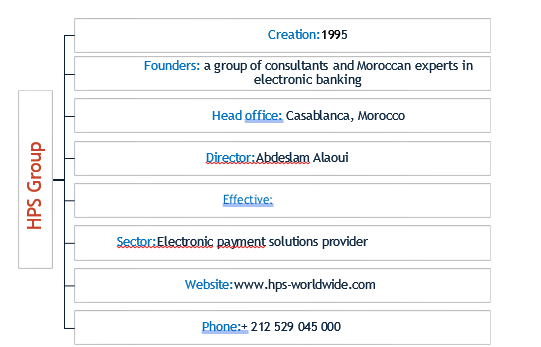
\includegraphics[width=5.41667in]{media/infosHPS.png}
\caption{HPS Morocco identity card}
\label{fig:infosHPS}
\end{figure}

Since its inception, HPS has continued to grow and diversify. The company began by providing credit and debit card processing solutions and gradually expanded its portfolio to include mobile payment, online payment, and risk management solutions. HPS has also expanded its international presence, with offices and clients in over 85 countries.
\end{quote}

\subsection{2 - HPS History :}

\begin{quote}
HPS was born from its founders' vision to create innovative and secure electronic payment solutions to meet the needs of financial institutions. From the very beginning, HPS focused on developing cutting-edge technologies and quickly gained recognition in the national market.

In 1999, HPS marked a milestone with the launch of PowerCard, an integrated payment platform that transformed the management of bank cards and payment transactions. This flagship product enabled HPS to expand its operations internationally, attracting customers in Africa, the Middle East, Europe, and Asia.

Over the years, HPS has continued to innovate and diversify its offerings, consolidating its leadership position in the payment technology sector. In 2010, the acquisition of ICPS (Indian Ocean Card Processing Services) strengthened its presence in the international market and expanded its client portfolio.

Today, HPS is recognized as a major player in the field of electronic payment solutions, with a presence in more than 90 countries and a diverse customer base including banks, financial institutions, and payment operators.
\end{quote}

\begin{figure}[H]
\centering
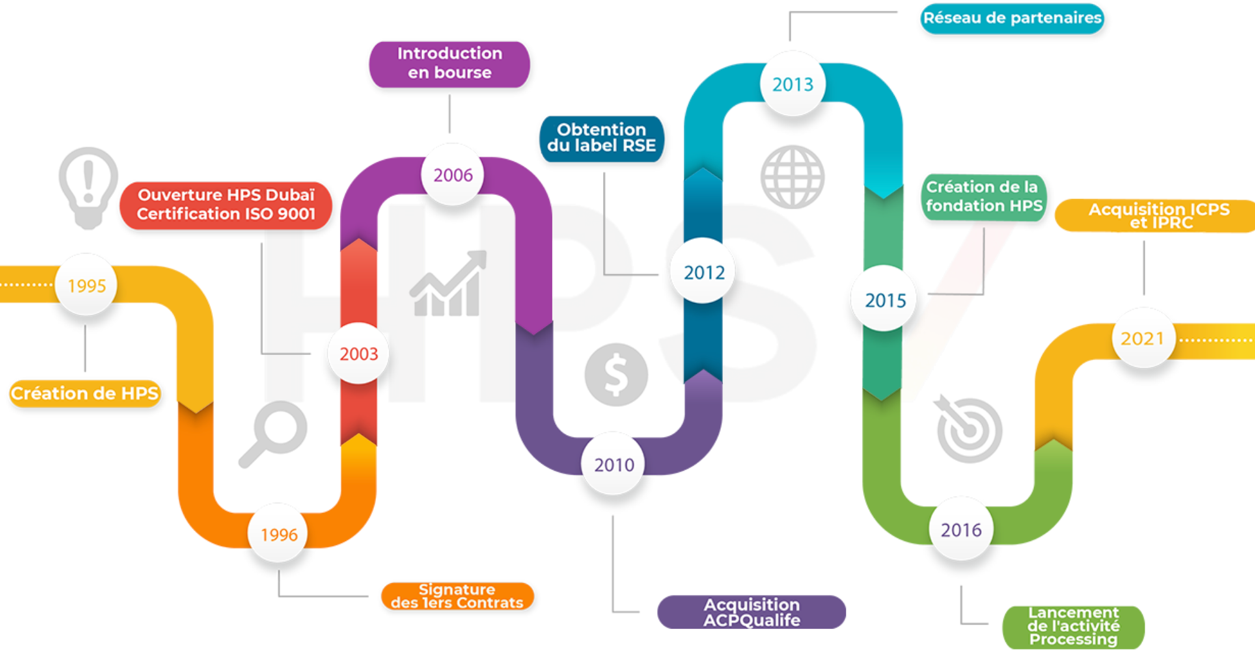
\includegraphics[width=5.7in]{media/image10.png}
\caption{HPS History}
\label{fig:hpsHistory}
\end{figure}

\subsection{3 - Main missions :}

\begin{quote}
HPS is the invisible technology that makes simple, transparent, and secure payments possible, allowing people to create, share, and live.

HPS enables the delivery of high-value solutions and services and ensures the smooth and secure execution of transactions across all possible payment channels and across all business sectors.

It is constantly working to enhance its suite of POWERCARD solutions for omnichannel electronic payment, which it deploys to its customers around the world.
\end{quote}

\clearpage
\subsection{4 - Main activities:}

\begin{figure}[H]
\centering
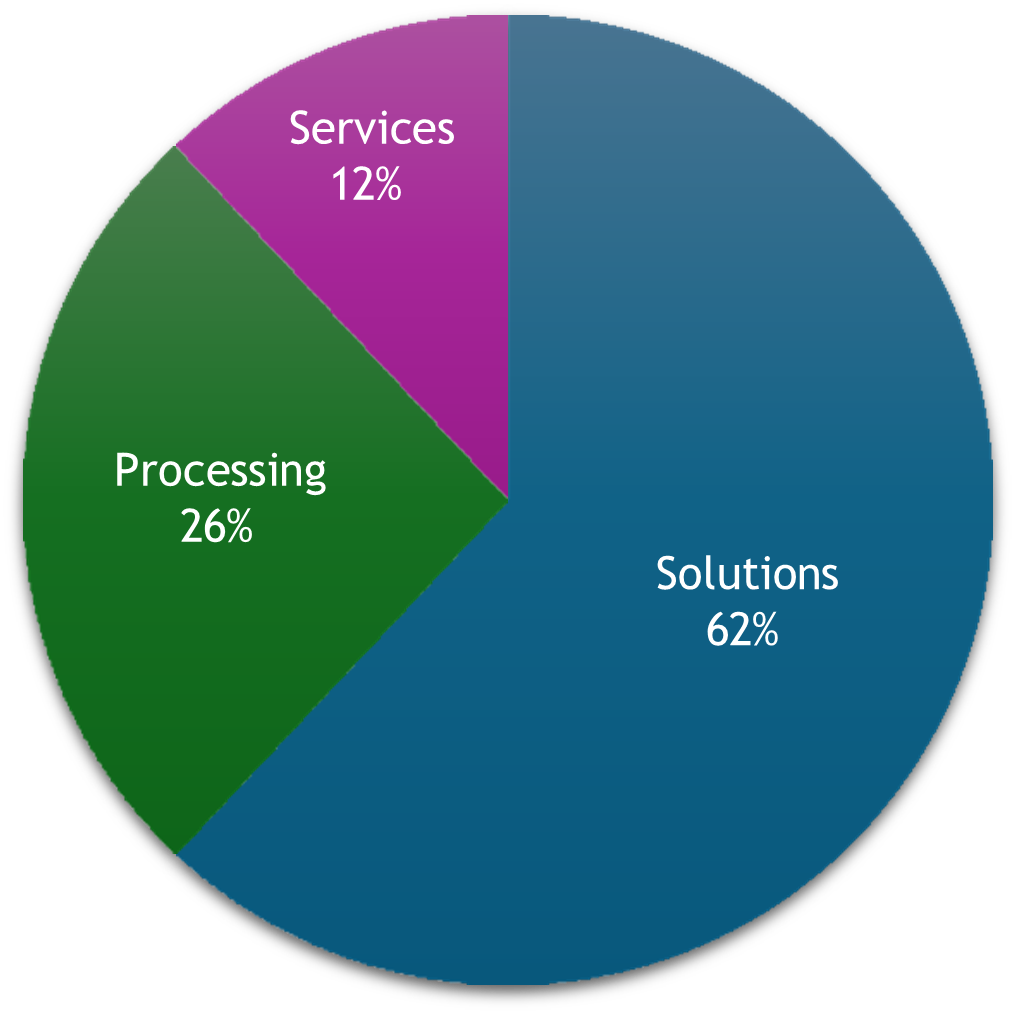
\includegraphics[width=2.5in]{media/spsHPS.png}
\caption{HPS activities}
\label{fig:spsHPS}
\end{figure}

\begin{quote}
Solutions: Omnichannel management of electronic payments in ``on-premise'' mode through PowerCard Solutions.

Processing: Management of national switching activities in Morocco and processing of transactions through the POWERCARD platform in SaaS mode.

Services: Testing, software qualification and project management assistance for IT transformation projects.
\end{quote}

\subsection{5 - Main products :}

\begin{quote}
\textbf{PowerCard:} It is a payment card and mobile payment management platform. PowerCard enables financial institutions to efficiently manage financial transactions, issue payment cards, and provide mobile payment services.

\textbf{SmartSwitch:} SmartSwitch is a payment switching solution that provides secure connectivity between financial sector stakeholders. It facilitates the routing of transactions between issuers, acquirers, and payment networks.

\textbf{PowerCard Connect:} This Payments Platform as a Service (PaaS) enables businesses to quickly launch customized payment services, reducing time to market.

\textbf{ePower:} ePower is a mobile payment solution developed by HPS to enable secure, contactless payments via smartphones.

\textbf{Switchware:} Switchware is a comprehensive product suite dedicated to payment management for banks and financial institutions.
\end{quote}

\subsection{6 - International presence :}

\begin{quote}
With offices in Africa, Europe, the Middle East, Asia, and North America, HPS is a truly global company. This international presence allows HPS to understand local specificities and offer solutions tailored to each market.
\end{quote}

\begin{figure}[H]
\centering
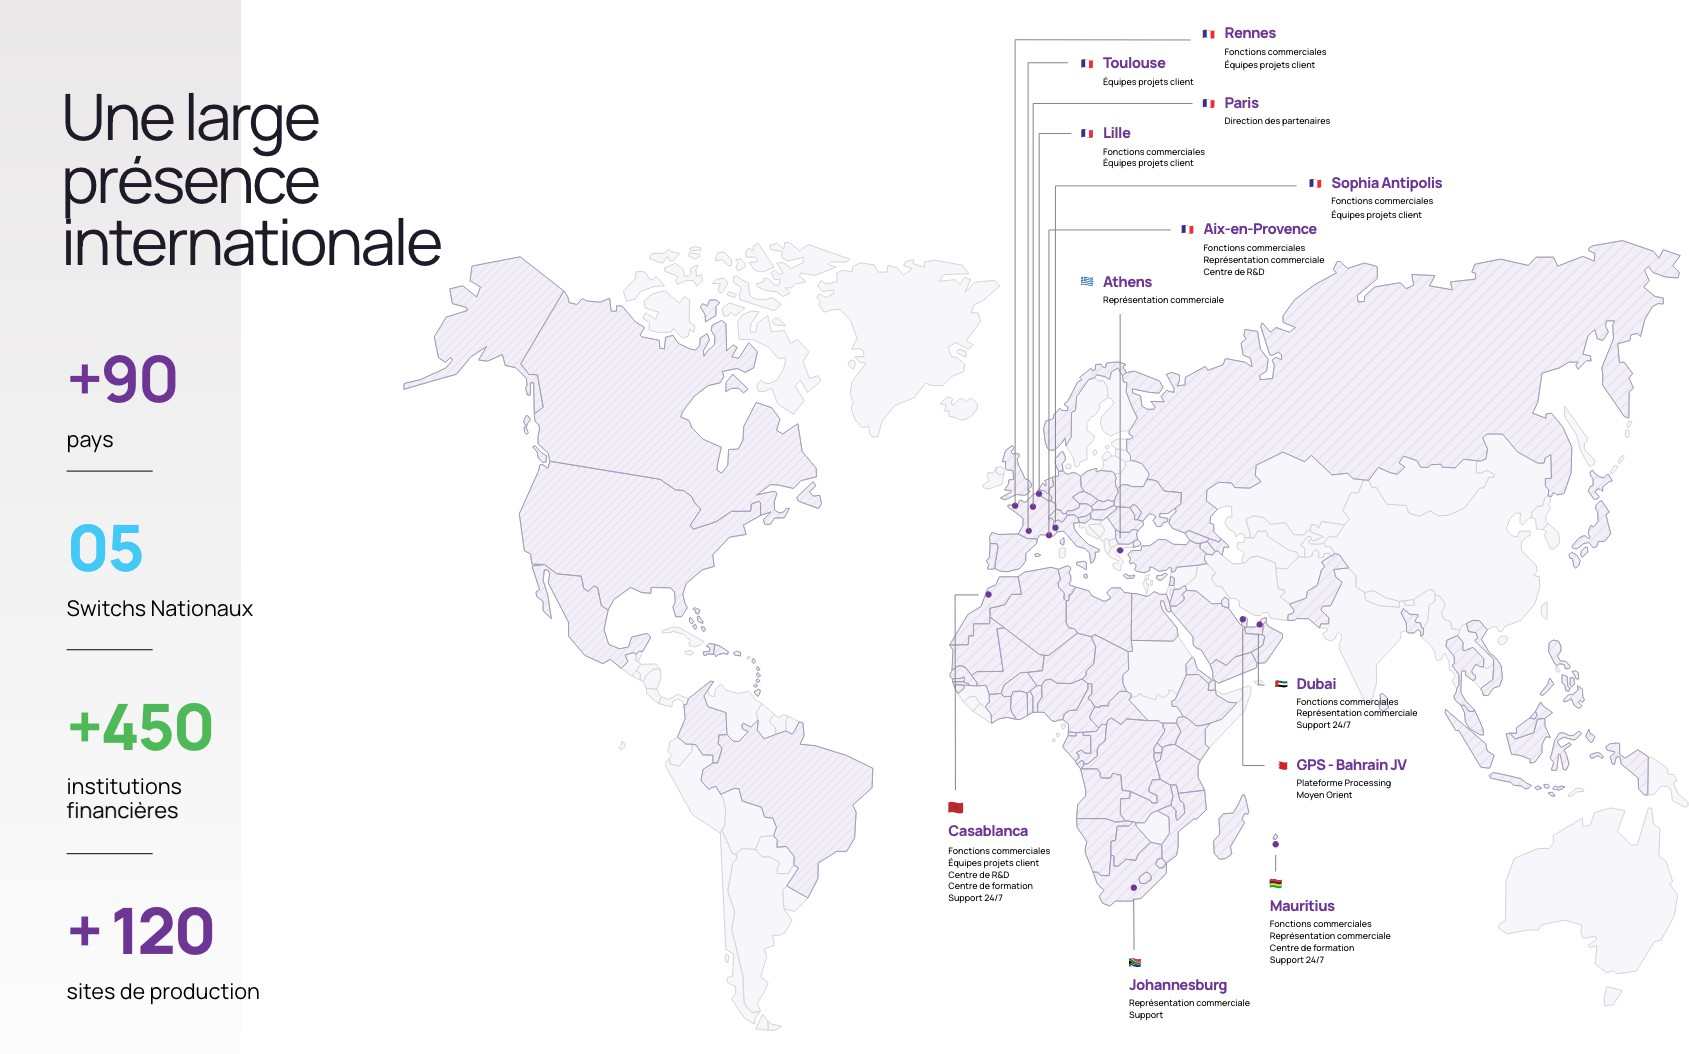
\includegraphics[width=6in]{media/image23.jpeg}
\caption{HPS International Presence}
\label{fig:intlPresence}
\end{figure}

\subsection{7 - Company organization chart :}

\begin{quote}
In 2021, the HPS Group adopted a new organization that takes into account its new dimension and its international development. This organization gives the various entities of the Group increasing autonomy and guarantees the achievement of several levels of synergies between them. It also highlights two essential aspects for the future evolution of the HPS Group: customer support and sales development through the Market entity, and management of the integration and development of PowerCard solutions in its different versions and according to the two models under the responsibility of the Software Factory entity.

Furthermore, the Group's new organization reflects the consolidation of the two activities previously grouped within Processing (Payment \& Switching), following their sustained development over the past few years, both organically and through acquisitions. HPS has thus set up the Payments Services entity, responsible for processing payment transactions and services related to its operations, and has given the Switching activity a dedicated entity to support the development of electronic payment at the national level. The Group has also strengthened the prerogatives of the Corporate Services entity, which has a central and transversal role, enriched by the new functions linked to external growth and the management of the Group's CSR issues. The operational deployment of the Group's strategic orientations and the monitoring of its performance are ensured by the Executive Committee under the supervision of the General Management, which also relies on the Transformation Committee, which oversees the implementation and supervision of the Group's transformation strategy.
\end{quote}

\begin{figure}[H]
\centering
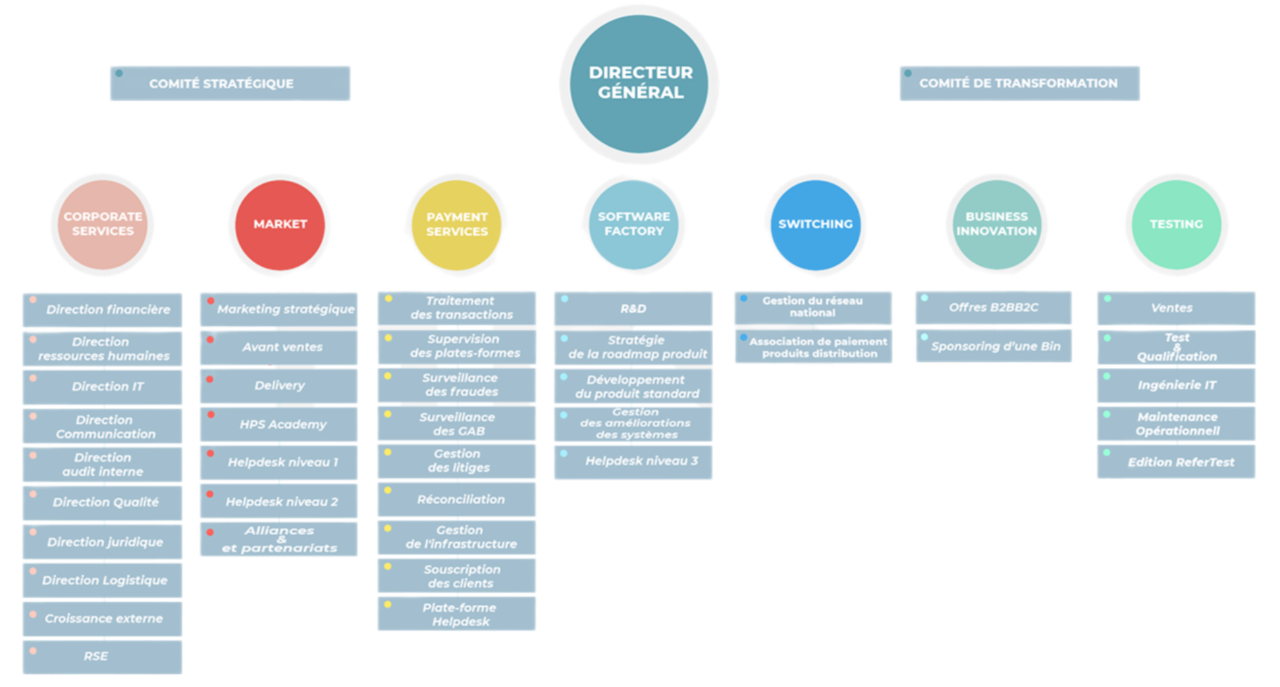
\includegraphics[width=6.4in]{media/image24.png}
\caption{HPS Organization Chart}
\label{fig:hpsOrgChart}
\end{figure}

\begin{figure}[H]
\centering
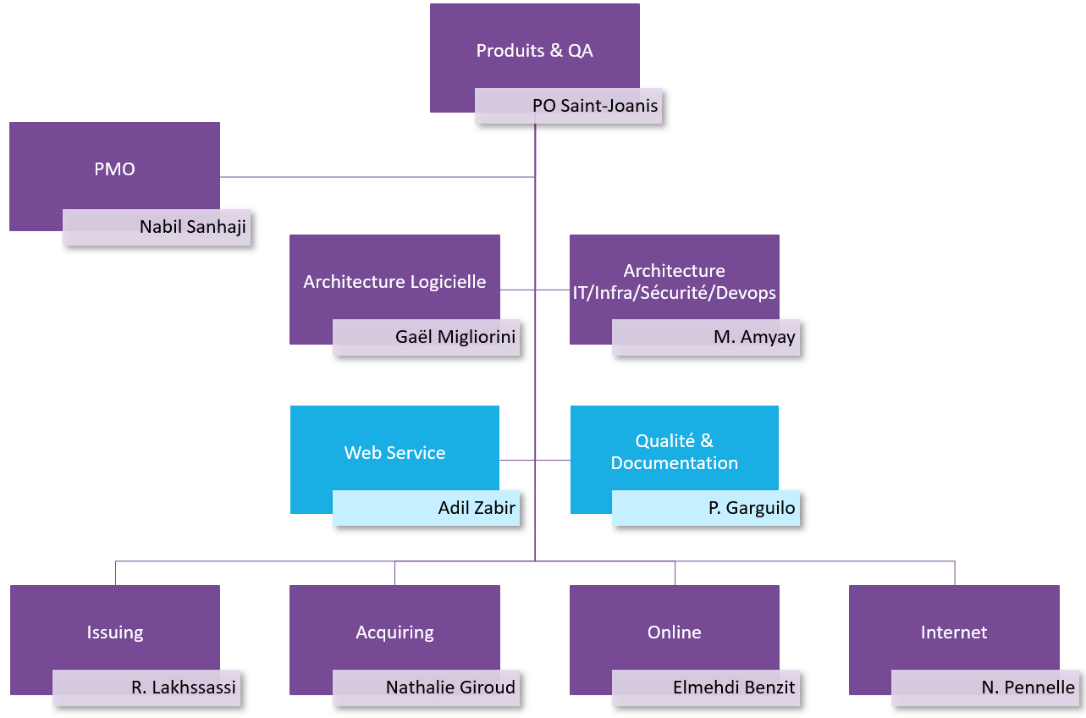
\includegraphics[width=6.4in]{media/image25.png}
\caption{HPS Organization Chart 2}
\label{fig:hpsOrgChart2}
\end{figure}

\subsection{8 - Presentation of the training :}

\begin{quote}
From our first day at HPS, the company offers us training on the principles and values of HPS, as well as self-training via the HPS-EACADEMY platform.

Regarding these training courses:
\end{quote}

\begin{itemize}
\item Introduction to the Payments Industry
\item Integration into the HPS Group
\item PowerCard Solutions
\item PCI DSS
\item Norms and standards
\end{itemize}

\begin{figure}[H]
\centering
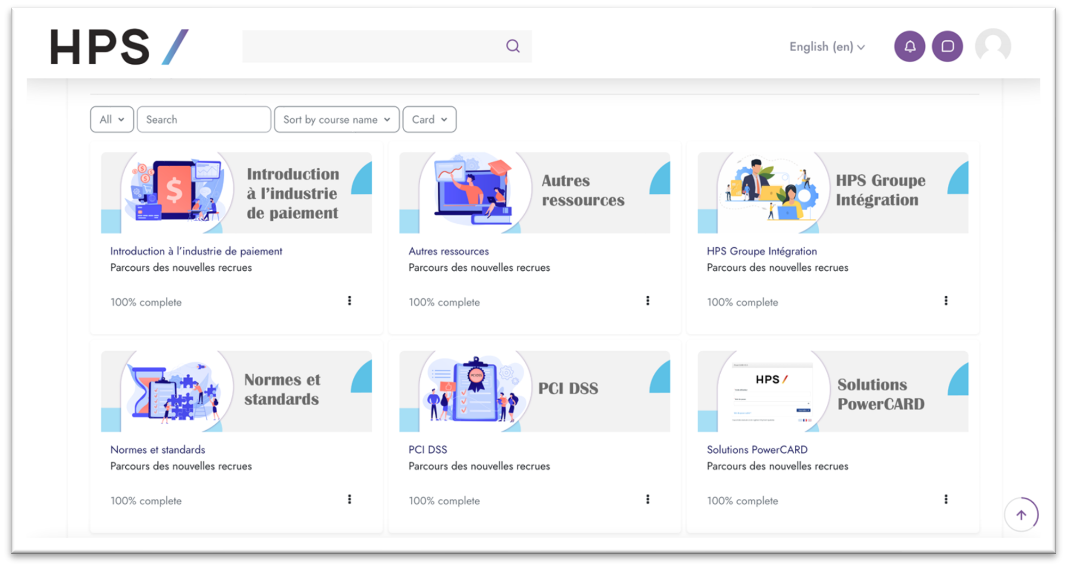
\includegraphics[width=4.8in]{media/image26.png}
\caption{HPS Training}
\label{fig:hpsTraining}
\end{figure}

\subsection{Conclusion :}
\begin{quote}
This chapter provided a comprehensive overview of the internship environment, introducing the host organization, its history, missions, core activities, and international presence. These elements helped to understand the framework in which the internship took place and the key aspects of the HPS company.
\end{quote}
\clearpage




% Chapter 2
\section{Chapter 2: General context of the
project :}
\subsection{Introduction}
\begin{quote}
The specification is the first step in a project. This step is crucial
for the smooth running of the project. It consists of knowing and
understanding the work required from an organizational and structural
point of view. In the first part, we will begin by presenting the
general context of the application by discussing the problem,
objectives, and scope. In the second part, we will present the work
methodology and planning.
\end{quote}


\subsection{1 - Fundamental concepts:}


\subsubsubsection{Cis (Customer Specification
Interface):}

\begin{quote}
This is Mastercard\textquotesingle s implementation of the ISO 8583-1987
standard for processing authorization information using the Mastercard
Dual Message System authorization platform. It provides Mastercard
customers with the information needed to develop a software interface
between Customer Processing Systems (CPS) and
Mastercard\textquotesingle s Dual Message System.
\end{quote}


\subsubsubsection{What is CIS Interface ? }
\begin{quote}
It is a Powercard interface designed to communicate with the Mastercard
network for online authorization management.
\end{quote}


\subsubsubsection{Where can the CIS interface be configured ?}

\begin{quote}
We can configure the CIS interface in PowerCard from the following
screen: Settings \textgreater{} PowerCARD-Switch \textgreater{} Switch
Settings \textgreater{} Resources \textgreater{} Definition
\textgreater{} Resource Settings

\textbf{What is the mapping between CIS protocol and Powercard internal
protocol?}

Here we find the mapping between the CIS protocol and the Powercard
protocol.

\begin{figure}[H]
\centering
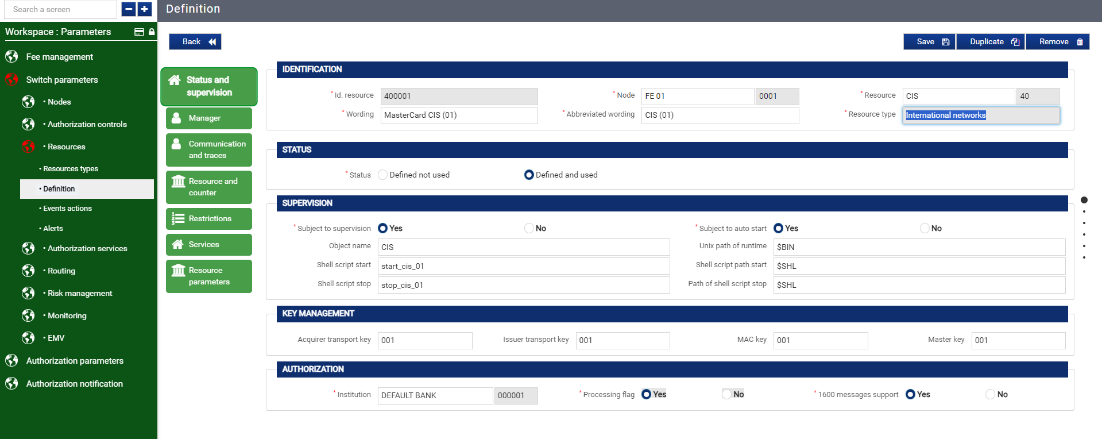
\includegraphics[width=6.4in]{media/image27.png}
\caption{HPS Organization Chart}
\label{fig:Issuer background}
\end{figure}

\end{quote}

\textbf{Issuer background}
\begin{quote}
As part of issuing an authorization request, Powercard uses the CIS
interface to capture and process incoming messages from MasterCard network, performing
the necessary security checks associated with the issuing party and the
mapping between the CIS protocol and the Powercard Switch protocol...
\end{quote}



\textbf{Acquirer background}

\begin{quote}
As part of acquiring an authorization request, Powercard uses the CIS
interface to process incoming messages from Mastercard Network, performing the
necessary security checks associated with the acquiring party and the
mapping between the Powercard Switch protocol and the CIS protocol...
\end{quote}


\subsubsubsection{Issuing and acquiring: }

\begin{quote}
\textbf{Issuing:}This is the bank that issued the
customer\textquotesingle s credit card. It is responsible for
authorizing or declining transactions.

\textbf{Acquiring :}This is the merchant\textquotesingle s bank, which
accepts card payments and relays authorization requests to the banking
network.
\end{quote}


\subsubsubsection{Simplified flow diagram :}

\begin{figure}[H]
\centering
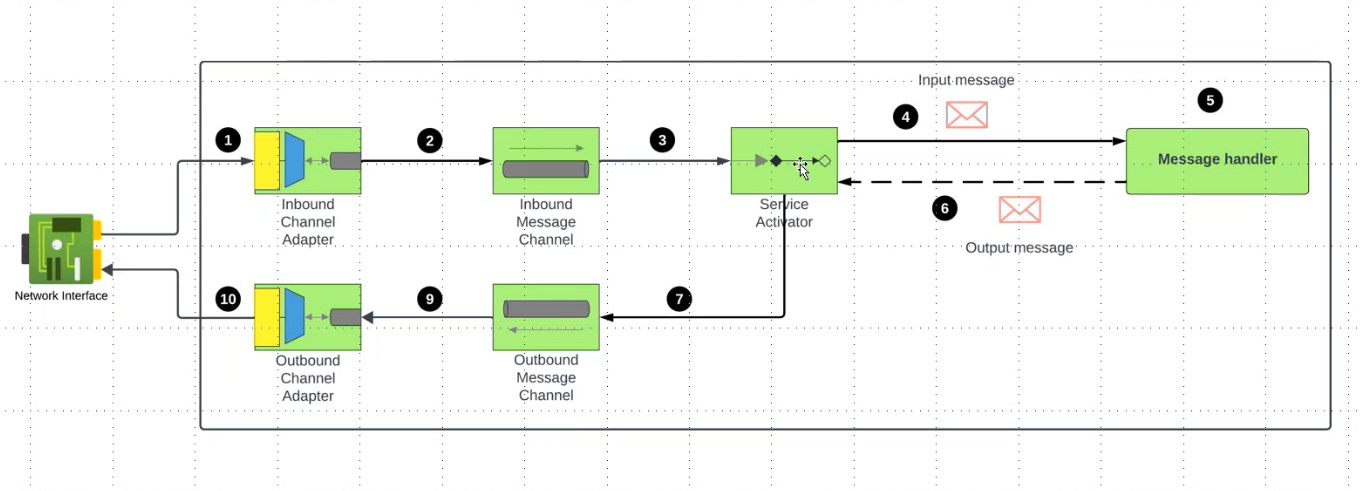
\includegraphics[width=5in]{media/image28.png}
\caption{Explanatory diagram of
the entry and exit of the message in tcp/ip}
\label{fig:fig9}
\end{figure}

\begin{quote}
Each received message starts with a structured header : the first 4 bytes
indicate the message length, followed by the protocol identifier (ISO),
the PowerCARD header, then the message type (MTI) and the
primary/secondary bitmaps that indicate the fields present. The data
fields follow this format: for example, field 2 (card number) is of type
LLVAR, field 3 (processing code) is fixed, field 4 (transaction amount)
is 12 digits. Some fields like field 48 (Private Additional Data) use a
TLV (Tag-Length-Value) encoding. The bitmap allows to know which fields
are present: if the i-th position is equal to 1, the i field is
included. This structure guarantees a clear and adaptable reading of
ISO8583 messages within PowerCARD.
\end{quote}


\begin{figure}[H]
\centering
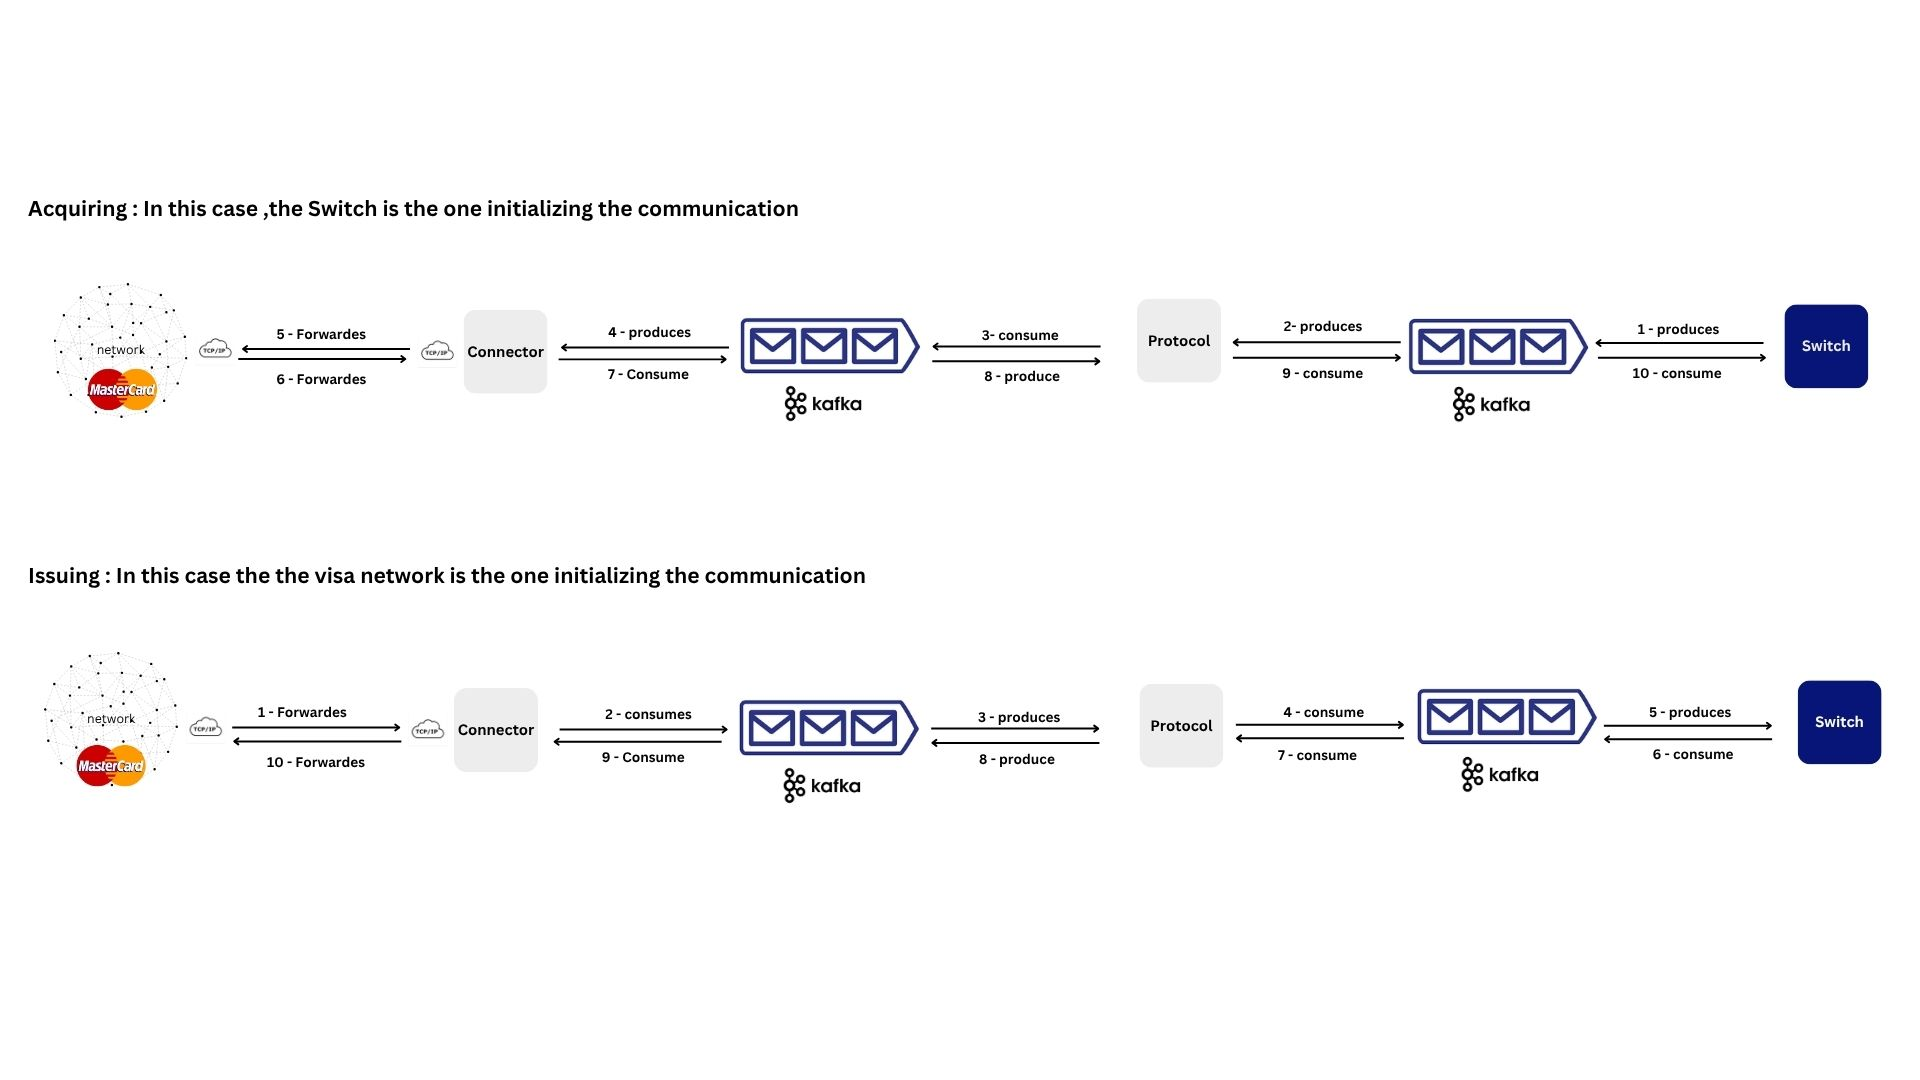
\includegraphics[width=1\textwidth]{media/image29.jpg}
\caption{Explanatory diagram
of the two message flows}
\label{figure}
\end{figure}

\begin{quote}
This figure illustrates the two possible communication flows between the
Mastercard network and the Switch via Channel V4:
\end{quote}

\begin{itemize}
\item
  \begin{quote}
  \textbf{In acquiring}: it is the Switch that initiates the
  communication. It generates a transaction message (Authorization,
  Reversal, Advice, File Upload ), which passes through Kafka to the Protocol service (where the ISO ↔ CIS mapping is performed), then passes through the Connector which sends the message to the Mastercard network. The response follows the reverse path.
  \end{quote}
\item
  \begin{quote}
  \textbf{In issuing}: here, it is the Mastercard network that
  initiates the communication. The incoming message first arrives at the The connector is passed to the Protocol for processing and mapping, and then injected into Kafka to be consumed by the Switch.
  \end{quote}
\end{itemize}

\begin{quote}
Kafka serves as an asynchronous messaging layer, enabling resilience and
traceability of flows between components.
\end{quote}


\subsubsubsection{What is digital banking ?}

\begin{quote}
Digital electronic banking refers to all technologies that enable
secure and traceable electronic payments. It includes bank cards,
payment terminals, electronic payment switches, networks (Visa,
Mastercard), and internal banking systems.
\end{quote}


\subsubsubsection{The main actors in the world of digital banking:}

\begin{quote}
The electronic money system is based on several actors who interact to
enable a secure transaction to be carried out:
\end{quote}

\begin{itemize}
\item
  \begin{quote}
  \textbf{The cardholder (the customer)}: it initiates the card
  transaction.
  \end{quote}
\item
  \begin{quote}
  \textbf{The merchant}: he receives payment via a payment terminal (TPE
  or ATM).
  \end{quote}
\item
  \begin{quote}
  \textbf{The acquiring bank}: it provides the payment infrastructure to
  the merchant.
  \end{quote}
\item
  \begin{quote}
  \textbf{The issuing bank (}\emph{\uline{issuer}}\textbf{)}: she issued
  the customer\textquotesingle s bank card.
  \end{quote}
\item
  \begin{quote}
  \textbf{The international network
  (}\emph{\uline{MasterCard}}\textbf{)}: it acts as a link between the
  two banks.
  \end{quote}
\end{itemize}

\begin{quote}
\textbf{The bank switch} (PowerCARD at HPS): it plays the role of
intermediary
\end{quote}


\subsubsubsection{How a transaction flows : }

\begin{quote}
When a customer makes a card payment:
\end{quote}

\begin{itemize}
\item
  \begin{quote}
  The terminal sends an authorization request (Request) to the acquiring
  bank.
  \end{quote}
\item
  \begin{quote}
  This request goes through the electronic money switch, which
  translates it into the correct format according to the network
  protocol (e.g.: CIS for Mastercard).
  \end{quote}
\item
  \begin{quote}
  The network (Mastercard) then transmits the message to the issuing
  bank (issuer).
  \end{quote}
\item
  \begin{quote}
  The issuer validates or rejects the transaction, then returns a
  response.
  \end{quote}
\item
  \begin{quote}
  This response is sent back to the merchant.
  \end{quote}
\end{itemize}


\subsubsubsection{Position of my solution in this ecosystem:}

\begin{quote}
The project I worked on aims to reimplement this channel in the form of
two modern microservices:
\end{quote}

\begin{itemize}
\item
  \begin{quote}
  \emph{\uline{Protocol}}: for the ISO ↔ CIS transformation logic
  \end{quote}
\item
  \begin{quote}
  \emph{\uline{Connector}}: for TCP/IP communication with the Mastercard
  network
  \end{quote}
\end{itemize}

\begin{quote}
\textbf{My role was to design and develop this smart gateway}, capable
of processing end-to-end flows:
\end{quote}

\begin{itemize}
\item
  \begin{quote}
  \textbf{Authorization}
  \end{quote}
\item
  \begin{quote}
  \textbf{Reversal}
  \end{quote}
\item
  \begin{quote}
  \textbf{Advice}
  \end{quote}
\item
  \begin{quote}
  \textbf{File Upload}
  \end{quote}
\end{itemize}

\begin{quote}
In other words, my solution acts as a banking interpreter, ensuring that
every message transmitted between actors follows the correct rules,
formats and protocols, while ensuring security and compliance.
\end{quote}


\subsubsubsection{The ISO 8583 protocol:}

\begin{itemize}
\item
  \textbf{Definition}
\end{itemize}

\begin{quote}
ISO 8583 is a standard communication protocol for exchanging financial
messages. It is used by most international networks (Visa, Mastercard,
Amex) for authorization requests.
\end{quote}

\begin{itemize}
\item
  \textbf{Structure of a message}
\end{itemize}

An ISO 8583 message is composed of three main parts:

\begin{quote}
\textbf{MTI (Message Type Indicator)}: a 4-digit numeric field
indicating the general function of the message (authorization request,
response, etc.)
\end{quote}


\begin{figure}[H]
\centering
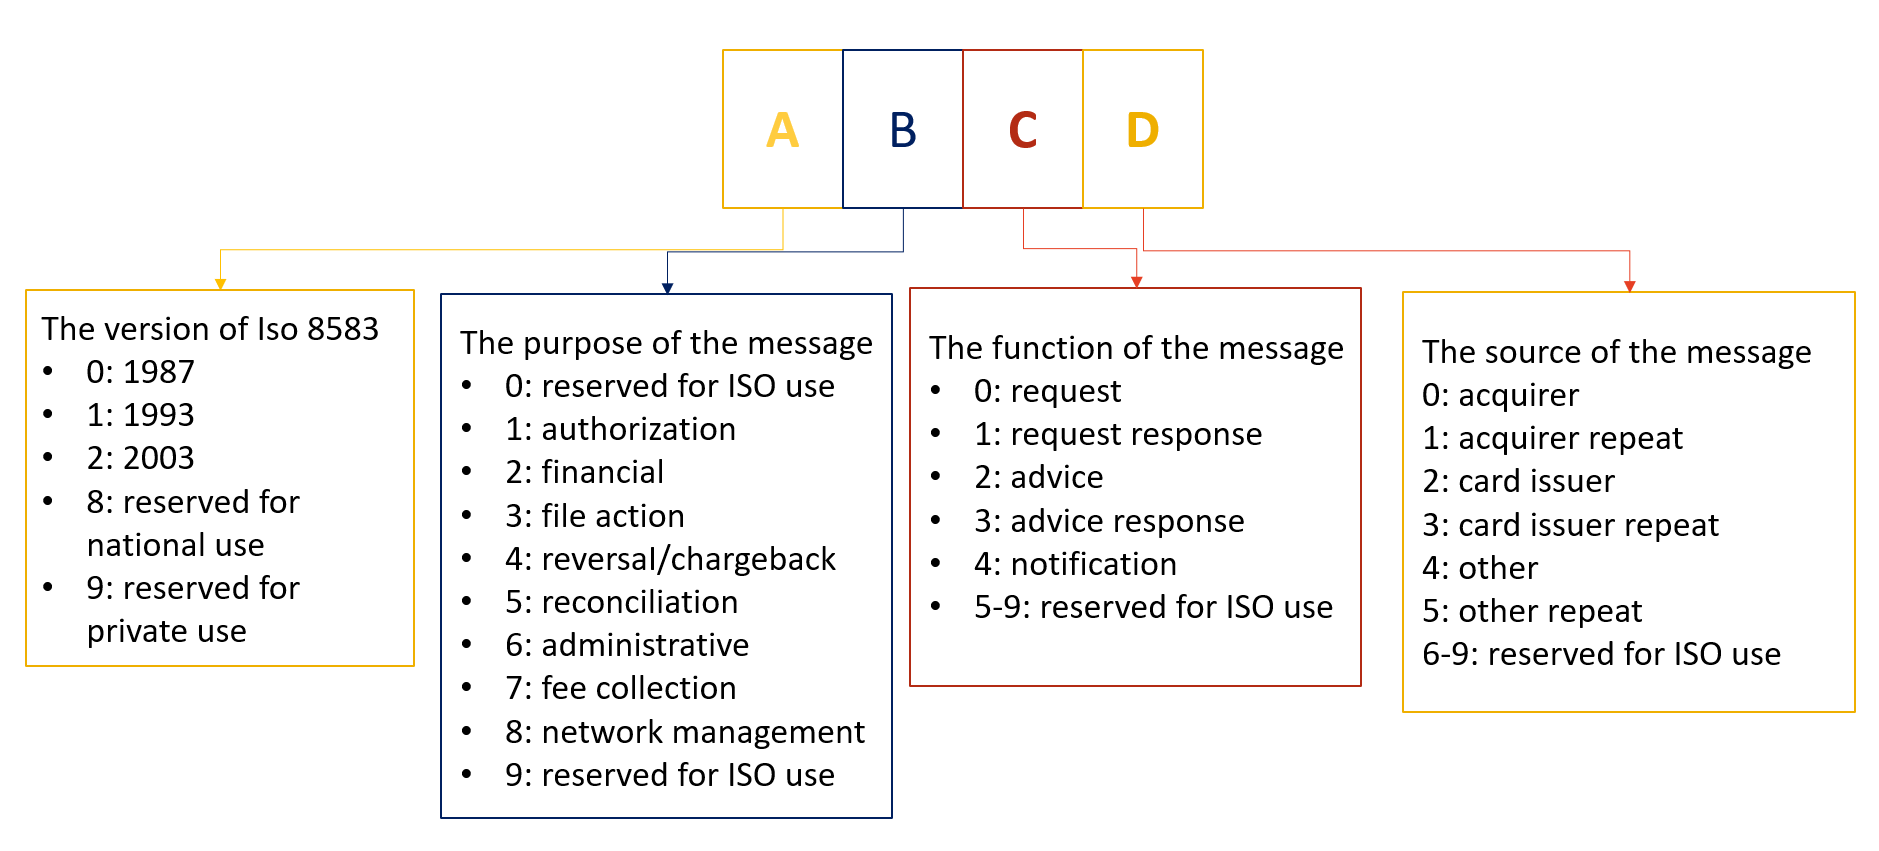
\includegraphics[width=6in]{media/image30.png}
\caption{Explanatory diagram of MTI }
\label{fig:hpsTraining}
\end{figure}

Bitmap: A bitmap is used to indicate the data elements present in a
message.

The main bitmap, consisting of 64 binary positions (16 in hexadecimal),
indicates whether a specific element is present (1) or absent (0).

There can be up to 192 data elements.

Data Elements: The fields containing the actual transactional data, such
as amount, PAN, response code, etc.

\begin{itemize}
\item
  \textbf{ISO-8583 Field Encoding~:}
\end{itemize}

\begin{quote}
\textbf{Undefined}: When an ISO-8583 standard field is not used in the
interface protocol, its type is defined as Undefined. Even if the field
is unused, all its properties must be declared so that, if it is
received in the authorization message, the parsing process knows to
ignore it and move on to the next field.

\textbf{TLV (type-length-value or tag-length-value)}:

The TLV-encoded data stream contains a code identifying the data
element, followed by the length of the record value, and then the value
itself. The tag and length are fixed-size (usually 1 to 4 bytes), and
the value field is variable-size. These fields are used as follows:

\emph{\uline{Tag}}: Binary or alphanumeric code identifying the field.

\emph{\uline{Length}}: Size of the field value (usually in bytes).

\emph{\uline{Value}}: A series of variable-sized bytes containing the
data for this part of the message.

\textbf{BER (Basic Coding Rules)}:

Is a set of rules specifying a standardized way to represent complex
data structures, such as integers, strings, and sequences, in binary
format.

TLV encoding can be considered as a specific application of BER, where
fixed sizes are assigned to the tag and length.

BER elements, such as field 55, use a TLV structure. Each BER element
consists of one or more bytes indicating the data type (tag) of the
element, one or more bytes indicating the length of the value, and the
encoded value itself.

\textbf{Bitmapped:}

Data encoding: Some fields use bitmap encoding to specify the
sub-elements present in the field. Each field using bitmap encoding
begins with a bitmap, with each bit representing a potential
sub-element. A bit set to "1" indicates that the corresponding
sub-element is included in the field; a "0" indicates its absence.

After the bitmap, the field contains the actual data for each
sub-element identified as present by the bitmap.

The main properties of bitmap-encoded fields are:
\end{quote}

\begin{itemize}
\item
  \begin{quote}
  Number of Bitmaps: Indicates the number of bitmap sequences used.
  \end{quote}
\item
  \begin{quote}
  Bitmap Length: Indicates the total number of bytes in each bitmap.
  \end{quote}
\item
  \begin{quote}
  Bitmap Format: Indicates whether the bitmap is encoded in ASCII or
  binary.
  \end{quote}
\end{itemize}

\begin{itemize}
\item
  \textbf{Channel Architecture V4: Abstract Layers}
\end{itemize}

\begin{quote}
Each V4 channel is based on three layers:
\end{quote}

\begin{itemize}
\item
  \begin{quote}
  \textbf{Abstract Layer}: analysis, logging, communication
  \end{quote}
\item
  \begin{quote}
  \textbf{Custom Layer}: ISO ↔ CIS mapping specific to each network
  \end{quote}
\item
  \begin{quote}
  \textbf{Configuration Layer}: security, addresses, formats
  \end{quote}
\end{itemize}

\begin{itemize}
\item
  \textbf{Internal Channel Services (Protocol/Connector)}
\end{itemize}
\clearpage


\textbf{Connector:}
\begin{figure}[H]
\centering
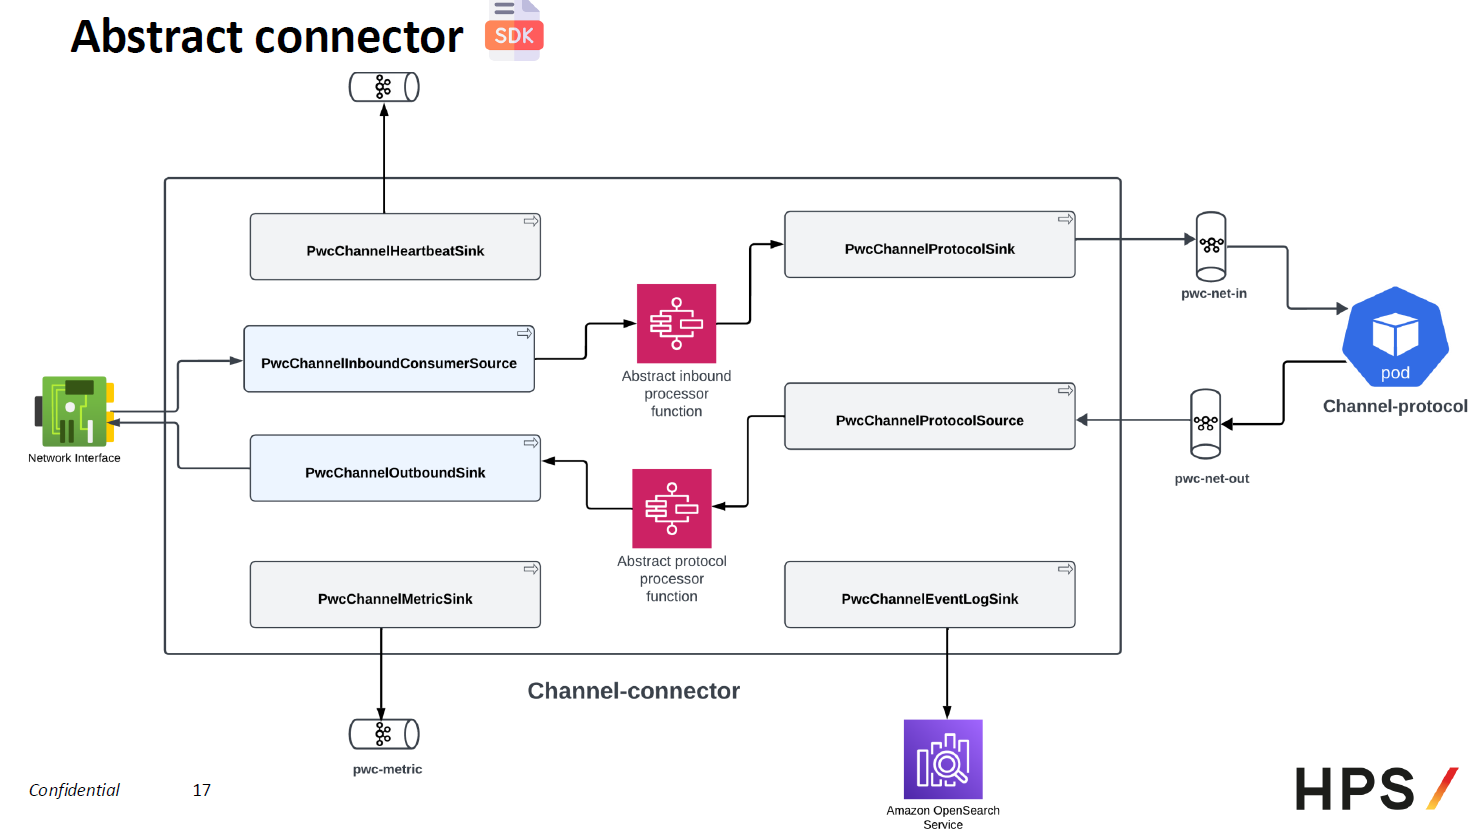
\includegraphics[width=6.31605in,height=3.54559in]{media/image31.png}
\caption{Diagram of the
structure of the abstract connector}
\label{fig:hpsTraining}
\end{figure}



\begin{itemize}
\item
  \begin{quote}
  Source: PwcChannelConnectorSource
  \end{quote}
\item
  \begin{quote}
  Processor: AbstractConnectorProcessorFunction
  \end{quote}
\item
  \begin{quote}
  Sink: PwcChannelPartitionerSink
  \end{quote}
\end{itemize}

\begin{quote}
\textbf{Main services:}

The connector relies on several essential components that ensure the
reliability, monitoring and observability of the service. The
PwcChannelHeartbeatSink component sends periodic signals (heartbeat) to
check the connector status (online / offline). The
PwcChannelEventLogSink logs service lifecycle events (start, sign-on,
stop, etc.). The PwcChannelMetricSink keeps track of important metrics,
such as message processing times. The PwcChannelContext stores
configuration information, the current state of the service and
associated metadata.\\
The embedded RocksDB database allows message and processing context
persistence, with TTL (time-to-live) based management. The OpenTelemetry
module provides advanced system traceability and observability
capabilities. Finally, the ChannelAdapter offers utilities for sending
network responses and updating connection status.
\end{quote}
\clearpage


  \textbf{Protocol}


\begin{figure}[H]
\centering
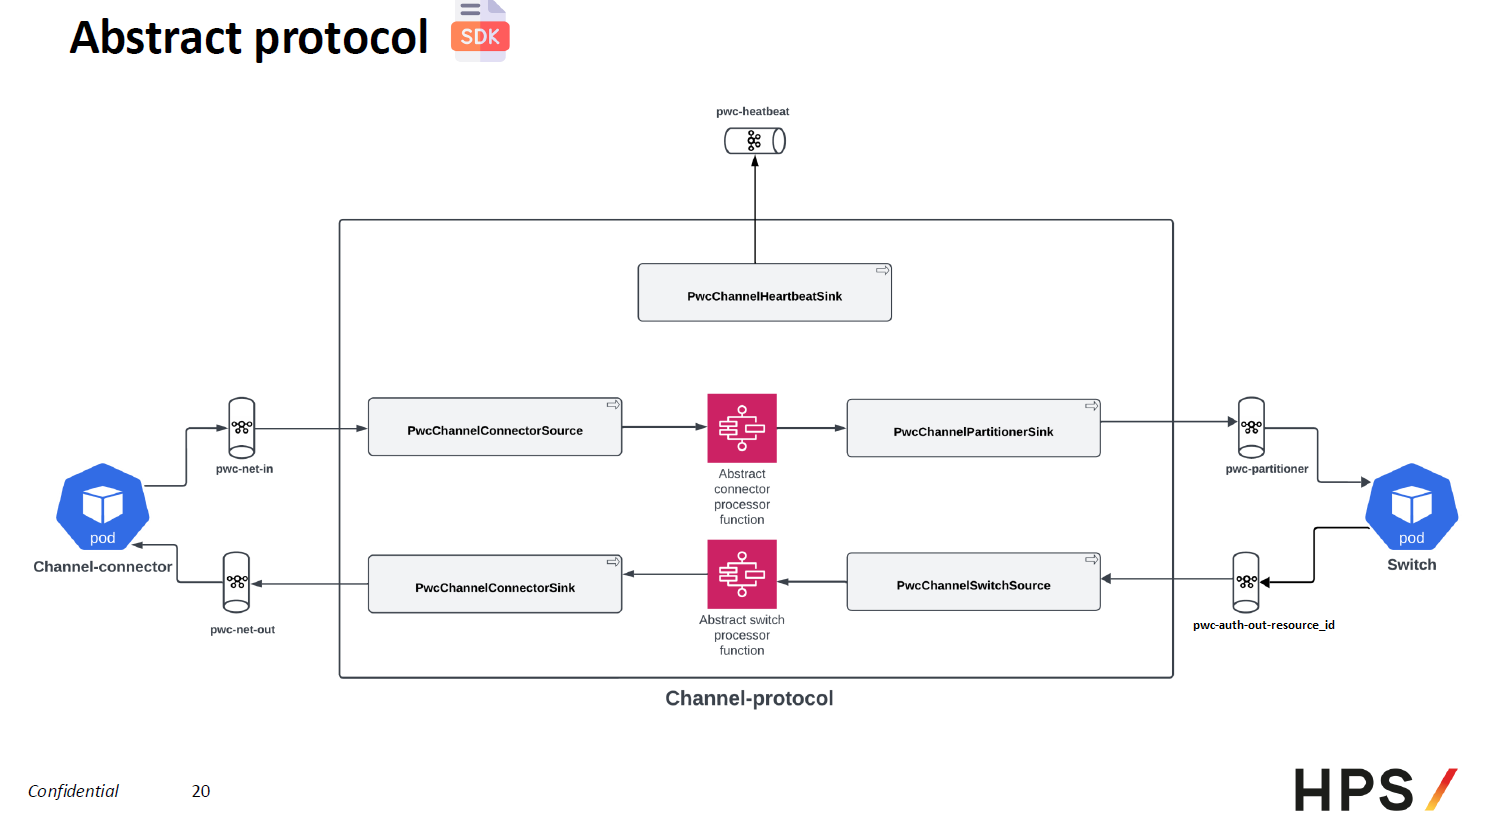
\includegraphics[width=6.31605in,height=3.54559in]{media/image32.png}
\caption{Diagram of the
structure of the abstract protocol}
\label{fig:diagramAbPo}
\end{figure}

\begin{itemize}
\item
  \begin{quote}
  Source: PwcChannelSwitchSource
  \end{quote}
\item
  \begin{quote}
  Processor: AbstractSwitchProcessorFunction
  \end{quote}
\item
  \begin{quote}
  Sink: PwcChannelConnectorSink
  \end{quote}
\end{itemize}

\begin{quote}
\textbf{Main services}
\end{quote}

\begin{itemize}
\item
  \begin{quote}
  \textbf{PwcChannelConnectorSource}: Receives authorization requests.
  \end{quote}
\item
  \begin{quote}
  \textbf{AbstractConnectorProcessorFunction}: Processes messages before
  sending them to the switch. This function is specific to each Channel.
  Developers must implement message type processing and protocol mapping
  by overloading the methods of the extended class.
  \end{quote}
\item
  \begin{quote}
  \textbf{PwcChannelPartitionerSink}: Sends messages to the appropriate
  partition of the switch.
  \end{quote}
\item
  \begin{quote}
  \textbf{PwcChannelSwitchSource}: Receives responses from the switch.
  \end{quote}
\item
  \begin{quote}
  \textbf{AbstractSwitchProcessorFunction}: Processes responses received
  from the switch. This function is specific to each Channel. Developers
  must implement message type processing and protocol mapping by
  overloading the methods of the extended class.
  \end{quote}
\item
  \begin{quote}
  \textbf{PwcChannelConnectorSink}: Sends the final response to the
  connector.
  \end{quote}
\item
  \begin{quote}
  \textbf{PwcChannel Heartbeat Sink}: Monitors the health of the
  protocol service.
  \end{quote}
\end{itemize}

\begin{quote}
\textbf{Features}
\end{quote}

\begin{itemize}
\item
  \begin{quote}
  Heartbeat and readiness check.
  \end{quote}
\item
  \begin{quote}
  TTL storage with RocksDB for message tracking.
  \end{quote}
\item
  \begin{quote}
  Propagation of channel context between connector, protocol and switch.
  \end{quote}
\item
  \begin{quote}
  Full integration with Kafka (connector ↔ protocol ↔ switch).
  \end{quote}
\item
  \begin{quote}
  Support for administration commands via gRPC.
  \end{quote}
\end{itemize}

\begin{itemize}
\item
  Connectivity with HSM module.
\item
  Observability thanks to OpenTelemetry.
\end{itemize}

\begin{quote}
\textbf{Other components:}
\end{quote}

\begin{itemize}
\item
  Heartbeat, Metrics, RocksDB, OpenTelemetry, HSM
\end{itemize}

\begin{itemize}
\item
  \textbf{The properties of a CIS message:}
\end{itemize}


\begin{figure}[H]
\centering
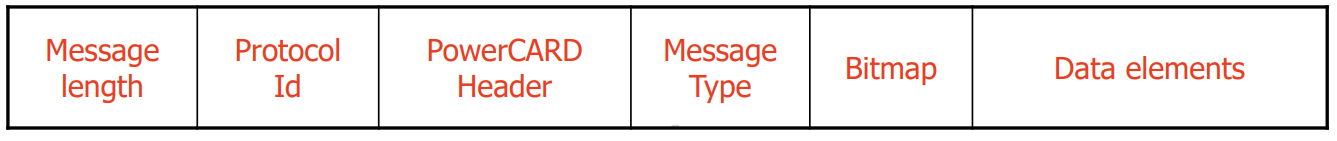
\includegraphics[width=6.31605in]{media/image33.png}
\caption{Diagram of the CIS
message structure}
\label{fig:DiagramMS}
\end{figure}


\begin{quote}
This diagram describes the structure of a message as it is processed in
the Mastercard CIS Channel. Each message begins with the total message
length (Message length), followed by the Protocol ID, and then the
PowerCARD header, which contains routing information.

Next is the Message Type (MTI), which defines the nature of the
transaction (authorization, reversal, file upload, advice, etc.). The
Bitmap specifies which data fields will be included in the message.

Finally, the Data Elements section contains all transactional
information (card number, dates, response codes, etc.). This structure
is essential to ensure the correct interpretation and compatibility of
messages between PowerCARD and the Mastercard network.
\end{quote}


\subsection{2 - Project context:}
\subsubsubsection{Problematic : }

\begin{quote}
Migrating the PowerCARD Switch CIS channel is a strategic imperative to
modernize the infrastructure and optimize communication with the
Mastercard network. The legacy implementation, developed in C, poses
major challenges in terms of security, maintainability, and integration
with the PowerCARD Switch V4 microservices architecture. Replacing C
with Java provides improved security and memory management, increased
developer productivity, simplified maintenance, and optimal platform
compatibility.

The existing C code, processing messages following the ISO 8583 standard
with Mastercard-specific variations, suffers from several critical
limitations: increased vulnerability due to manual memory management, a
lack of integration with modern microservice technologies (Kafka, gRPC),
and high maintenance costs of Docker images due to the need for frequent
updates to fix security vulnerabilities and ensure library
compatibility. In addition, the scarcity of C++ developers familiar with
these modern technologies makes maintaining and evolving this code
particularly challenging.

As part of the migration of the PowerCARD Channel solution from version
4 implemented in C to a version 4 rewritten in Java, the integration of
the CIS channel is therefore essential. The move to Java/Spring Boot
will provide automatic memory management, a rich ecosystem of libraries
and tools, better exception handling, and increased portability thanks
to the JVM. This migration is crucial to ensure compliance with the
latest Mastercard standards, reduce security risks, and enable the rapid
introduction of new financial services.

\emph{\uline{The Switch team, in charge of this development, is facing
two major technical difficulties:}}

The complexity of processing encoded fields: Many message fields use
encoding formats such as TLV (Tag-Length-Value) or BER (Basic Encoding
Rules). To facilitate the identification of these formats, the team
designed a solution based on an XML file, which acts as a data
dictionary, describing all the message fields. This XML file does not
automatically process the encoding; it provides the information
necessary to determine the format (TLV, BER, etc.) and apply the
appropriate decoding routines. The combination of this XML file, the
detailed documentation (Confluence) and CIS protocol documentation, and
the developers\textquotesingle{} expertise in translating business logic
from C code to Java, will allow for an efficient and accurate migration.

The complexity of CIS protocol specifications: The CIS channel reference
documents are dense, sometimes unclear, and difficult to use directly.
Optimal use of the specifications requires in-depth knowledge of
existing code and accurate interpretation of the technical documents.

The central challenge of this report is therefore to migrate the CIS
channel to a modern, secure, and maintainable version, taking full
advantage of the benefits of Java and microservices architecture, while
overcoming the challenges related to the complexity of encoding formats
and CIS protocol specifications. The success of this migration is
essential to ensure fast, reliable, and secure communication with the
Mastercard network and to ensure the future evolution of the PowerCARD
Switch platform.
\end{quote}


\subsubsubsection{Project objective:}

\begin{quote}
The PowerCARD Switch Customer Interface Specifications (CIS) channel
migration project from its current C language implementation to a new
Java version has the following objectives.
\begin{itemize}
\item
  \emph{Modernize the technical infrastructure}: Replacing monolithic C code with a Java/Spring Boot microservices architecture to improve the flexibility, scalability and resilience of the PowerCARD Switch platform.

\item
  \emph{Improve code maintainability and security}: Benefit from Java's advantages in terms of automatic memory management, exception handling, and a rich ecosystem of libraries and development tools, thus reducing the risk of vulnerabilities and facilitating long-term maintenance.

\item
  \emph{Ensure seamless integration with existing architecture}: Ensure optimal interoperability between the CIS channel and other Java/Spring Boot microservices of PowerCARD Switch V4, by adopting consistent communication and integration standards.

\item
  \emph{Simplify the processing of ISO 8583 messages}: Implement tools and processes to facilitate the identification and processing of encoded fields (TLV, BER, etc.), by using the XML field description file and capitalizing on the team’s expertise.

\item
  \emph{Optimizing communication with the Mastercard network}: Ensure fast, reliable and secure communication with the Mastercard network, in compliance with the latest CIS protocol standards and specifications.

\item
  \emph{Reduce maintenance and operating costs}: Reduce costs associated with maintaining Docker images and resolving security vulnerabilities, through the use of Java and modern development practices.
\end{itemize}

\end{quote}

\begin{quote}
Achieving these objectives will ensure the sustainability of the
PowerCARD Switch platform, improve its operational efficiency and ensure
its ability to meet the future needs of the electronic payments market.
\end{quote}
\clearpage

\subsubsubsection{Study of the existing situation :}
\textbf{Description of the existing}
\begin{quote}
The current Mastercard CIS message processing system is based on a
monolithic architecture developed in C language, integrated into the
PowerCARD V4 ecosystem. This historical solution provided the mapping
between PowerCARD\textquotesingle s internal ISO 8583 format and
Mastercard\textquotesingle s CIS protocol, used primarily in the
processing of authorization, confirmation, file and reconciliation
messages.

Although functional, this implementation currently suffers from several
structural limitations. The rigid architecture makes maintenance,
scalability, and integration with modern components such as Kafka,
Docker, or Kubernetes difficult. Additionally, message processing is
tightly coupled to the core of the system, making it difficult to add
new business rules or third-party protocols.

The environment does not allow for fine-grained transaction traceability
or smooth error management, which limits the system\textquotesingle s
resilience, particularly in the event of load peaks or partial failures.
\end{quote}

\begin{quote}
The main shortcomings of the V4 architecture are:
\begin{itemize}
\item
  \textbf{Strong coupling of business and network code}: ISO ↔ CIS
  processing is mixed with TCP communication logic, making the code
  difficult to modify or test independently.
\item
  \textbf{Low scalability}: Monolithic architecture limits the ability
  to process large volumes or adapt to load peaks.
\item
  \textbf{Obsolete technology}: The C language does not allow for smooth
  integration with modern tools such as Kafka, OpenTelemetry, or cloud
  monitoring solutions.
\item
  \textbf{Lack of modularity}: Every change in the protocol requires
  recompiling and redeploying the entire binary, which slows down
  responsiveness.
\item
  \textbf{Complex maintenance}: Requires C-skilled developers with good
  knowledge of legacy code.
\end{itemize}
\end{quote}

\subsubsubsection{Proposed solution :}

\begin{quote}
The solution is to migrate the Mastercard CIS channel to a microservices
architecture in Java Spring Boot, compatible with the PowerCARD V4
version.
This new architecture is based on two independent microservices:
\begin{itemize}
\item
  \textbf{Protocol}: responsible for CIS ↔ ISO 8583 mapping and business
  logic.
\item
  \textbf{Connector}: in charge of TCP/IP network communication with
  Mastercard.
\end{itemize}

\end{quote}



\begin{quote}
    \textbf{The advantages of this solution are numerous:}
    \begin{itemize}
\item
  \textbf{Separation of responsibilities}: Business processing is
  completely separated from network logic.
\item
  \textbf{Native integration with Kafka}: For asynchronous, traceable
  and resilient communication between services.
\item
  \textbf{Flexible deployment via Docker/Kubernetes}: For cloud-native
  management and horizontal scalability.
\item
  \textbf{Reusability via SDK}: Critical functions (TLV, TranslatePIN,
  etc.) are centralized in maintainable SDKs.
\item
  \textbf{Modern observability}: Integration with OpenTelemetry,
  centralized logs, and real-time monitoring.
\end{itemize}
\end{quote}



\begin{quote}
This migration represents a fundamental architectural change, making the
system more flexible, scalable and ready for future protocols such as
BASE1 or MDS.
\end{quote}

\subsubsubsection{Indicative planning :}

\begin{quote}
The Mastercard CIS Channel migration project to a Java Spring Boot
architecture followed a progressive and iterative development cycle,
structured around learning the legacy system in C, implementing new Java
components, integration testing and stabilization.

The project officially started on February 24, 2025. I took over the
code on February 25, followed by an in-depth functional and technical
analysis phase, during which I explored the mechanisms of the C code, in
particular the functions that manage requests and responses in broadcast
mode.

Following this phase, I began implementing the Connector microservice,
then quickly implementing the Protocol, after clarifying the use of the
TLV format. The development of the Issuing flow (request and response)
was carried out in this first step.

During May, I started processing the Acquiring flow, developing the
function to convert request message from internal iso to external iso
and same function but for response conversion.

In parallel, the test environment was set up with Docker and Kubernetes,
allowing the reception of the Country and AcquirerID and Mcc tables, and
the execution of integration tests on the implemented flows.

As the academic defense approaches at the end of July, the Authorization
flows have been stabilized, and development has been focused on the
remaining flows: Reversal, Advice and File Upload, the full
implementation of which is planned after the defense.
\end{quote}

\begin{figure}[H]
\centering
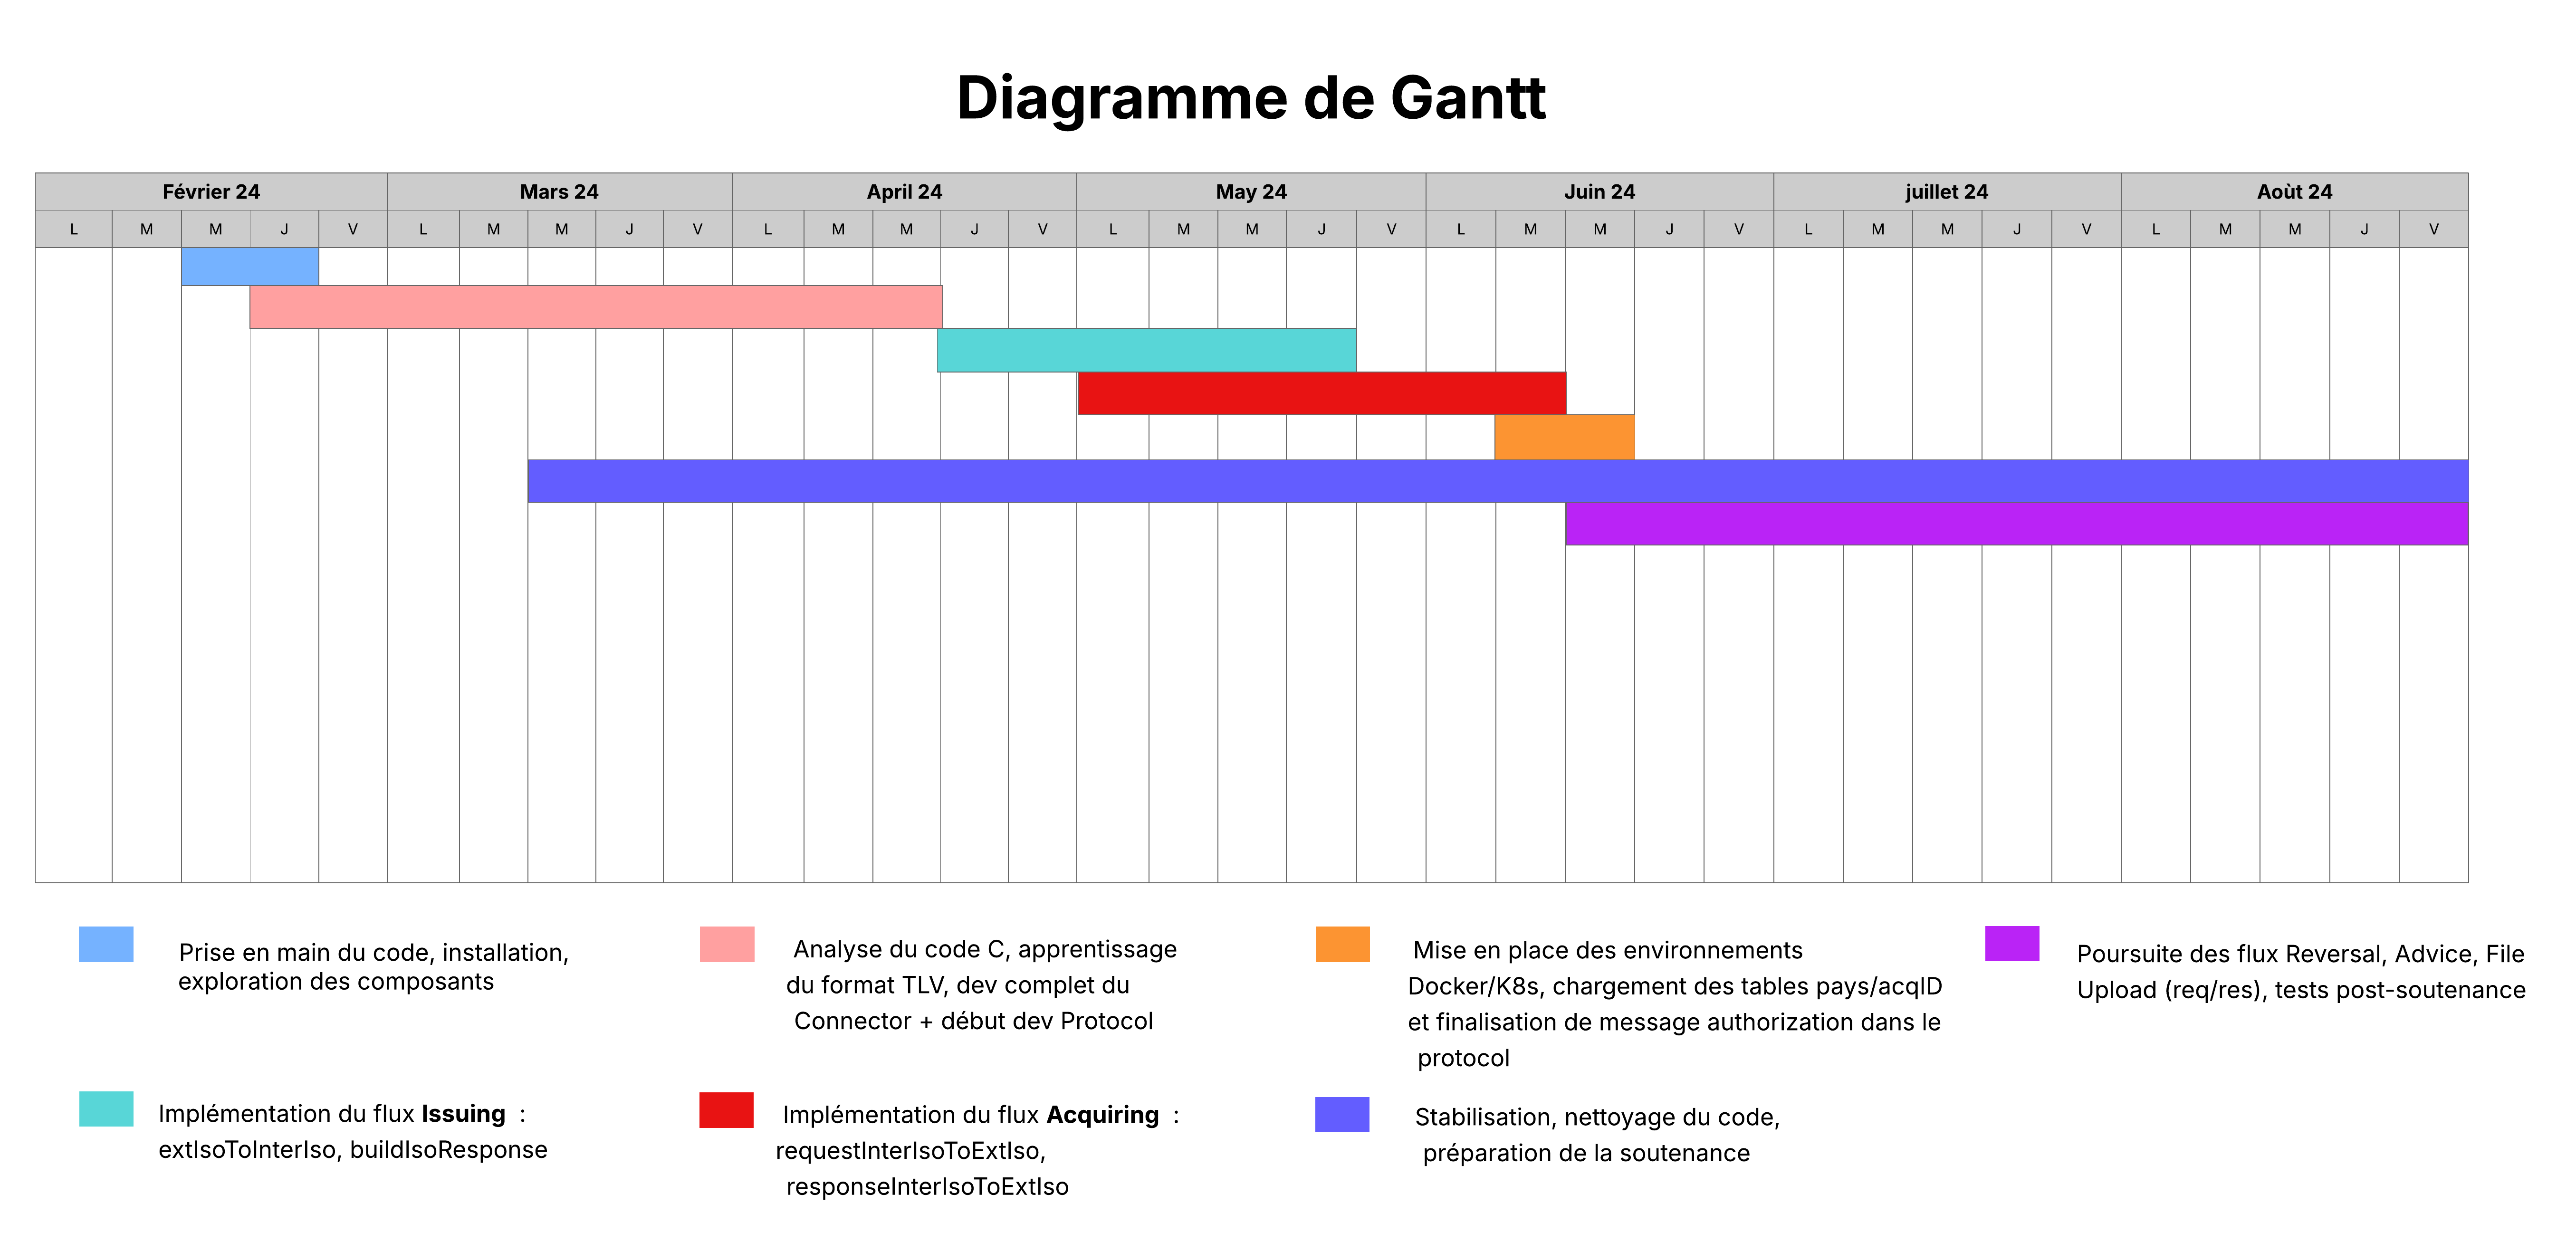
\includegraphics[width=6.31605in,height=3.54559in]{media/image34.png}
\caption{Gantt Chart Diagram}
\label{fig:gantt}
\end{figure}


\subsection{Conclusion : }
\begin{quote}
This second chapter laid the conceptual and technical foundations for
the Mastercard CIS Channel migration project to a modern Java Spring
Boot microservices architecture. It detailed the challenges of the
existing system, the critical limitations of the C implementation, and
the functional, technological, and strategic challenges of this
transformation.

The study of the existing system highlighted the obstacles related to
maintenance, scalability, and integration, which are hindering the
system\textquotesingle s evolution. In response, the proposed solution
based on the separation of responsibilities via Protocol and Connector
microservices, the integration of Kafka, and the implementation of a
reusable CIS SDK allows for the establishment of a more modular,
scalable architecture that complies with modern standards.

The technological choices and the adopted development model guarantee an
efficient and sustainable migration, capable of meeting business
requirements while preparing the PowerCARD platform for the integration
of future protocols.

This chapter thus constitutes the theoretical basis on which the
implementation phase, presented in the following chapter, was based.
\end{quote}
\clearpage

% Chapter 3
\section{Chapter 3: Project Analysis and Design}

\subsection{Introduction}
\begin{quote}
This chapter presents the functional analysis and business design of the
Mastercard CIS Channel Migration Solution. Its objective is to describe
the role of the solution in the overall flow of transactions, the
positioning of the main components (Protocol and Connector), as well as
the circulation of messages between the different stakeholders of the
system (Switch, Mastercard network, issuing banks and acquirers).

The chapter is based on flowcharts and abstract diagrams to explain the
expected operation of the solution, without addressing here the
technological choices or aspects related to implementation patterns.
\end{quote}


\subsection{1 - Analysis :}
\subsubsubsection{Functional requirements :}
\begin{quote}
This section describes the functional requirements of the new PowerCARD
Switch Customer Interface Specifications (CIS) channel, focusing on the
key components: Message Management, Connector, Protocol, and CIS SDK.

\emph{\uline{Message management:}}

The system must support the processing of all message types, in both
streams (acquisition and emission), whether requests or responses. The
main message types include:
\begin{itemize}
\item
  \begin{quote}
  \emph{Authorisation}: Request for authorization for a transaction
  (payment, withdrawal, etc.).
  \end{quote}
\item
  \begin{quote}
  \emph{Advice}: Notification without prior authorization.
  \end{quote}
\item
  \begin{quote}
  \emph{Reversal}: Cancellation of a previously granted authorization.
  \end{quote}
\item
  \begin{quote}
  \emph{File Upload}: Deferred transmission of batches of transactions.
  \end{quote}
\end{itemize}
\end{quote}



\begin{quote}
\emph{\uline{Connector:}}
The Connector is responsible for communication with the Mastercard
network and must ensure the following functionalities:
\begin{itemize}
\item
  \begin{quote}
  \emph{Network Communication}: Ensure communication with the Mastercard
  payment system.
  \end{quote}
\item
  \begin{quote}
  \emph{Timeout Management}: Manage network message timeouts using a
  deferred queue.
  \end{quote}
\item
  \begin{quote}
  \emph{Initial Connection}: Send an initial sign-on message.
  \end{quote}
\item
  \begin{quote}
  \emph{Heartbeat Management}: Manage heartbeats for liveness and
  readiness monitoring.
  \end{quote}
\item
  \begin{quote}
  \emph{Echo Tests}: Manage echo tests using a scheduler.
  \end{quote}
\item
  \begin{quote}
  \emph{Connection Tracking}TCP/IP: Monitor TCP/IP connections.
  \end{quote}
\item
  \begin{quote}
  \emph{Channel Event Management}: Manage channel events (start, stop,
  etc.).
  \end{quote}
\item
  \begin{quote}
  \emph{Channel Metrics Management}: Collect channel metrics, including
  response time.
  \end{quote}
\item
  \begin{quote}
  \emph{Observability}: Integrate OpenTelemetry for observability.
  \end{quote}
\item
  \begin{quote}
  \emph{Access to Configuration}: Provide a channel context giving
  access to the channel configuration.
  \end{quote}
\item
  \begin{quote}
  \emph{Channel Adapter}: Provide a channel adapter providing access to
  main functions.
  \end{quote}
\item
  \begin{quote}
  Context Persistence: Ensure context persistence using RocksDB to save
  CID (Channel Identifier) \hspace{0pt}\hspace{0pt}and OpenTelemetry
  data to correlate requests and responses.
  \end{quote}
\item
  \begin{quote}
  \emph{Kafka Communication}: Ensure communication with the Protocol
  component via Kafka.
  \end{quote}
\item
  \begin{quote}
  \emph{Administration Order Management}: Manage administrative commands
  using gRPC communication.
  \end{quote}
\item
  \begin{quote}
  \emph{TCP/IP Event Interceptor}: Intercept TCP/IP events.
  \end{quote}
\end{itemize}
\end{quote}



\begin{quote}
\emph{\uline{Protocol:}}

The Protocol is responsible for processing messages and communicating
with the Switch and must provide the following functionalities:
\begin{itemize}
\item
  \begin{quote}
  \emph{Managing Original Messages}: Manage incoming and outgoing
  original messages using RocksDB-based Time-To-Live (TTL) storage.
  \end{quote}
\item
  \begin{quote}
  \emph{Heartbeat Management}: Manage heartbeats for liveness and
  readiness monitoring.
  \end{quote}
\item
  \begin{quote}
  \emph{Context Propagation}: Propagate the channel context between the
  Connector, the Protocol and the Switch.
  \end{quote}
\item
  \begin{quote}
  \emph{Observability}: Integrate OpenTelemetry for observability.
  \end{quote}
\item
  \begin{quote}
  \emph{Access to Configuration}: Provide a channel context giving
  access to the channel configuration.
  \end{quote}
\item
  \begin{quote}
  \emph{Channel Adapter}: Provide a channel adapter providing access to
  main functions.
  \end{quote}
\item
  \begin{quote}
  \emph{Kafka communication (Connector)}: Ensure communication with the
  Connector component via Kafka.
  \end{quote}
\item
  \begin{quote}
  \emph{Kafka Communication (Switch)}: Ensure communication with the
  Switch via Kafka.
  \end{quote}
\item
  \begin{quote}
  \emph{HSM Connectivity}: Ensure connectivity with a Hardware Security
  Module (HSM).
  \end{quote}
\item
  \begin{quote}
  Administration Command Management: Manage administration commands
  using gRPC communication.
  \end{quote}
\item
  \begin{quote}
  \emph{Field Mapping}: Perform mapping of all message fields.
  \end{quote}
\end{itemize}
\end{quote}



\begin{quote}
\emph{\uline{CIS SDK:}}

The CIS SDK provides tools and functions to facilitate the development
and integration of the CIS channel and must ensure the following
functionalities:
\begin{itemize}
\item
  \begin{quote}
  \emph{Field Mapping:}
  \end{quote}

  \begin{itemize}
  \item
    \begin{quote}
    Manage message field mapping.
    \end{quote}
  \item
    \begin{quote}
    Process files requiring specific processing (via Protocol).
    \end{quote}
  \end{itemize}
\item
  \begin{quote}
  \emph{Unimplemented Functions}: Handle unsupported cases
  (unimplemented function).
  \end{quote}
\item
  \begin{quote}
  \emph{Special Cases:}Handle exceptions in fields.
  \end{quote}
\item
  \begin{quote}
  \emph{Resources}: Provide enumerations and configurations (CIS fields,
  network messages, special param loader, ...).
  \end{quote}
\end{itemize}
\end{quote}



\subsubsubsection{Non functional requirements:}

\begin{quote}
This section describes the non-functional requirements for the new
PowerCARD Switch CIS channel. These requirements define the expected
qualities and characteristics of the system, independent of its specific
functions.

\emph{\uline{Maintainability}}: The system must be easy to maintain,
modify and evolve, with clear, modular and well-documented code, thus
minimizing long-term maintenance costs.

\emph{\uline{Security}}: The system must ensure the security of data and
transactions, protecting against unauthorized access, vulnerabilities,
and potential attacks. This involves robust authentication mechanisms,
encryption of sensitive data, and access management.

\emph{\uline{Testability}}: The system must be easily testable at all
levels (unit, integration, system), with mechanisms to automate tests
and ensure code quality.

\emph{\uline{Reliability}}: The system must be reliable and available,
minimizing downtime and ensuring service continuity. This involves error
management, redundancy, and disaster recovery mechanisms.

\emph{\uline{Productivity}}: The system must enable high developer
productivity, by offering efficient tools and frameworks, as well as
clear and complete documentation.

Integrability: The system must integrate easily with other components of
the PowerCARD Switch architecture, respecting integration standards and
protocols.

\emph{\uline{Scalability}}: The system must be scalable, that is,
capable of handling an increasing workload without performance
degradation. This requires an architecture capable of adapting to
variations in traffic and resources.

\emph{\uline{Observability}}: The system must be observable, that is,
capable of providing detailed information about its state and operation,
thus allowing for rapid diagnosis of problems and optimization of
performance. This involves the collection of metrics, logs, and traces.
\end{quote}


\subsubsubsection{Use case diagram:}
\begin{quote}
    \textbf{Actor}
\end{quote}
\begin{quote}
As part of the migration of the Mastercard CIS Channel to the V4
architecture, the main players identified are:
\begin{itemize}
\item
  \begin{quote}
  \textbf{Mastercard Network}: the external network that exchanges
  messages with our system via the CIS protocol, using TCP/IP
  communication.
  \end{quote}
\item
  \begin{quote}
  \textbf{Switch (PowerCARD)}: the internal microservice that receives
  or sends ISO 8583 messages to financial institutions (issuing or
  acquiring banks).
  \end{quote}
\end{itemize}
\end{quote}



\begin{quote}
These two actors interact directly with the Mastercard CIS Channel,
which acts as a translator and router between the two message formats.
\end{quote}

\textbf{Main use cases}

\begin{quote}
The main use cases that structure the operation of the solution are:
\begin{itemize}
\item
  \begin{quote}
  \textbf{Process an incoming message from the Mastercard network}
  \end{quote}

  \begin{itemize}
  \item
    Receive a CIS message via the Connector
  \item
    Map the CIS message to an internal ISO 8583 format via the Protocol
  \item
    Transmit the mapped message to the Switch
  \end{itemize}
\end{itemize}

\begin{itemize}
\item
  \begin{quote}
  \textbf{Process an outgoing message from the Switch}
  \end{quote}

  \begin{itemize}
  \item
    Receive an internal ISO 8583 message via the Protocol
  \item
    Map ISO 8583 message to CIS format
  \item
    Send the mapped message to the Mastercard network via the Connector
  \end{itemize}
\end{itemize}
\end{quote}



\begin{quote}
These use cases cover all expected functional flows, whether
authorization, reversal, advice or file upload messages.
\end{quote}

\begin{quote}
    \textbf{Use Case Diagram:}
\end{quote}

\begin{quote}
The diagram above illustrates the main use cases of the Mastercard CIS
Channel (V4) in the context of the migration carried out.
\end{quote}

\begin{figure}[H]
\centering
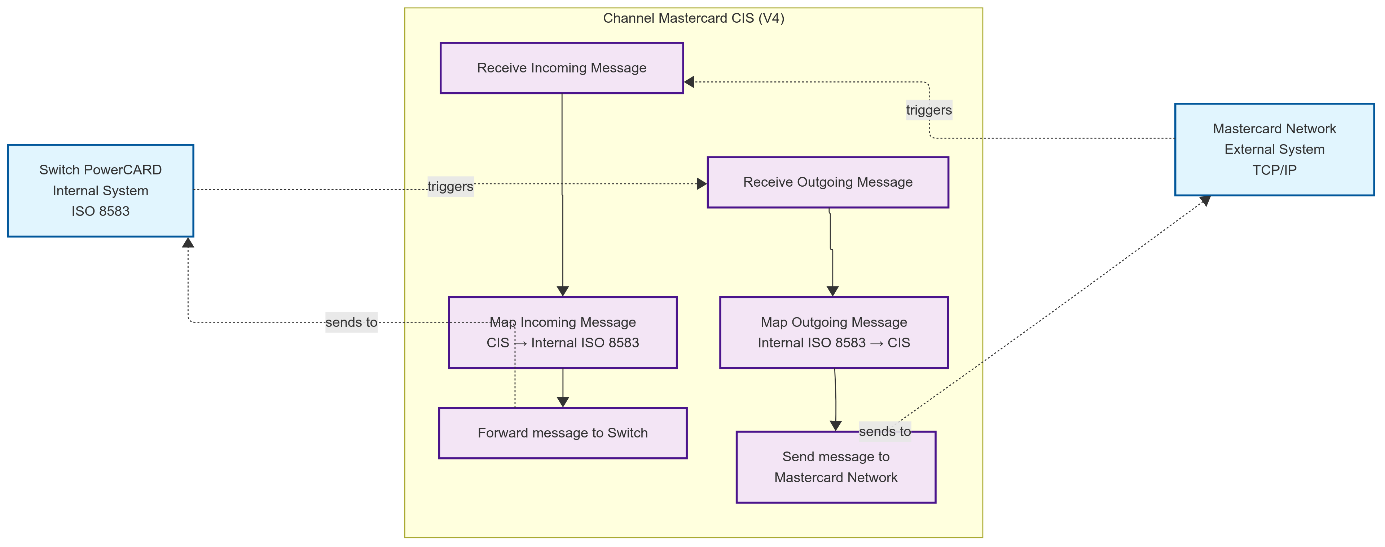
\includegraphics[width=7in]{media/image35.png}
\caption{Use Case Diagram Schema}
\label{fig:UseCaseD}
\end{figure}


\begin{quote}
The system is positioned between two main actors: on one side, the
Mastercard network (external actor) which communicates via a CIS
protocol encapsulated on TCP/IP; on the other, the PowerCARD Switch
(internal actor) which manages exchanges with financial institutions in
ISO 8583 format.

\textbf{\uline{Two major functional scenarios are represented:}}
\end{quote}

\begin{itemize}
\item
  \textbf{Incoming flow (Acquiring)} : The Mastercard network initiates
  communication by sending a CIS message. The Connector receives it
  (Receive Incoming Message), then the Protocol performs a detailed
  mapping (Map Incoming Message CIS → Internal ISO 8583), taking into
  account the business rules and the specificities of the internal
  protocol. The message thus transformed is then transferred to the
  Switch (Forward message to Switch), which processes it or relays it to
  the relevant bank.
\item
  \textbf{Outgoing flow (Issuing)} : Here, the PowerCARD Switch
  initiates the request (authorization, reversal, advice, etc.). The ISO
  message is sent to the Protocol (Receive Outgoing Message), where it
  is converted to the CIS format expected by Mastercard (Map Outgoing
  Message Internal ISO 8583 → CIS). The Connector then ensures the
  message is sent to the Mastercard network (Send message to Mastercard
  Network).
\end{itemize}

\begin{quote}
This diagram highlights the bidirectional nature of the Channel, which
acts as a translator between two heterogeneous protocol worlds, while
ensuring the conformity of the exchanged messages. It also illustrates
the logical independence of the Protocol and Connector components, each
assuming a specific role in the processing chain.
\end{quote}

\subsubsubsection{Sequence diagram :}
\textbf{General acquiring case:}
\begin{figure}[H]
\centering
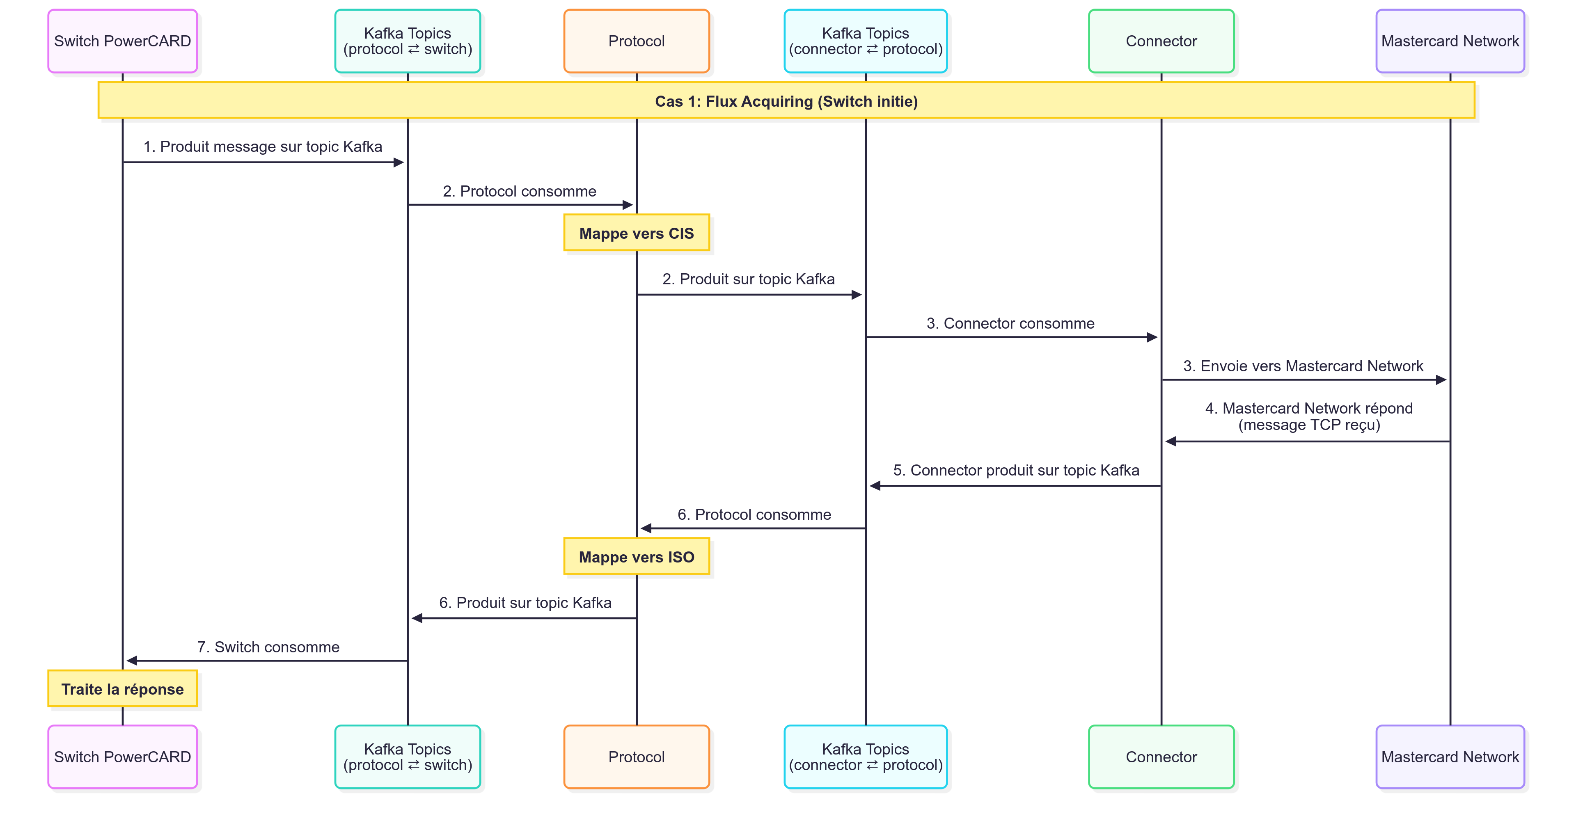
\includegraphics[width=6.13862in,height=2.76042in]{media/image36.png}
\caption{General Sequence Diagram}
\label{fig:gantt}
\end{figure}
% \clearpage

\begin{quote}
The presented diagram illustrates the complete flow of an Acquiring
authorization message in the migrated PowerCARD to Mastercard CIS
architecture, initiated by the Switch.

This case corresponds to a purchase transaction carried out by a
cardholder with a merchant (POS, e-commerce), where the PowerCARD Switch
initiates the flow to the Mastercard network.

\textbf{Step 1: Generate the authorization message}

The PowerCARD Switch generates an internal ISO 8583 authorization
message, corresponding to a transaction processing request (purchase,
authorization).

This message is published on a specific Kafka topic (protocol ↔ switch
topic), facilitating communication between the Switch and the protocol
module (Protocol).

\textbf{Step 2: Consumption and transformation to CIS}

The Protocol consumes this message and transforms it into the CIS format
used by the Mastercard network.

This mapping is achieved through a complex business logic
BuildAutReqToNw inspired by C code migrated to Java.

The produced CIS message is then published to a second Kafka topic
(connector ↔ protocol) to allow the Connector to use it.

\textbf{Step 3: Network Transmission}

The Connector consumes this CIS message and physically transmits it to
the Mastercard network via TCP communication (socket).

This layer provides encapsulation, session management, timeouts, and
network compliance.

\textbf{Step 4: Mastercard Network Response}

The Mastercard network processes the request and returns a response (TCP
message received by the Connector), which will be consumed and
transformed into a return.

\textbf{Step 5: Publication of the CIS response}

The Connector produces a CIS response message on the Kafka topic
(connector ↔ protocol).

\textbf{Step 6: Remapping to ISO}

The Protocol consumes the CIS response and transforms it back into the
internal ISO 8583 format, understandable by the Switch.

\textbf{Step 7: Processing by the Switch}

The PowerCARD Switch consumes this ISO response and processes it
(validation, database update, return to the POS or e-commerce).
\end{quote}
\clearpage

\begin{quote}
 \textbf{General issuing case:}   
\end{quote}

\begin{figure}[H]
\centering
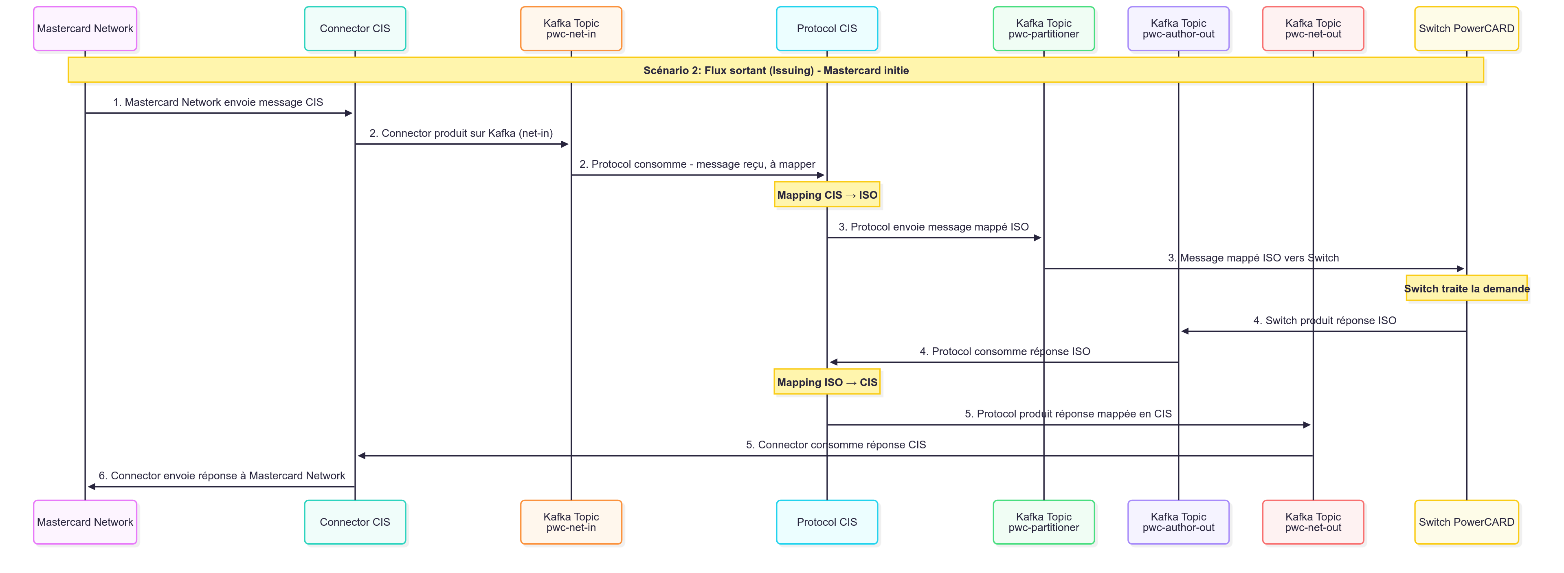
\includegraphics[width=7.10423in,height=2.60249in]{media/image37.png}
\caption{Sequence diagram of emission case}
\label{fig:SDEC}
\end{figure}

\begin{quote}
This diagram illustrates the flow of a request initiated by the
Mastercard network to PowerCARD in Issuing mode (Switch acting as the
card issuer).

In this case, it is the Mastercard network that sends an incoming
message to the PowerCARD Switch (for example an Advice 0120 or a
Reversal 0420).

Detailed procedure:

\textbf{Step 1: Receiving the network message}

The Mastercard Network sends a CIS message (Mastercard format) in TCP
mode to the CIS Connector.

\textbf{Step 2: Publish to Kafka}

The Connector receives this message, transforms it into a Kafka message
and publishes it to the pwc-net-in Kafka topic.

\textbf{Step 3: Consumption by Protocol}

The CIS Protocol consumes this Kafka pwc-net-in message.

It performs a CIS → ISO mapping (eg: BuildAutReqFromNw or
ReversalReqFromNw) to convert the CIS message into the internal ISO 8583
format, usable by PowerCARD.

The ISO mapped message is then published to the pwc-author-out topic.

\textbf{Step 4: Switch consumes the request}

The PowerCARD Switch consumes this ISO message.

It performs the corresponding business processing (authorization update,
balance check, database modification, etc.).

The Switch then produces an ISO 8583 response, which is published to the
Kafka topic pwc-net-out.

\textbf{Step 5: ISO → CIS Remapping}

The CIS Protocol consumes this ISO response, and performs an ISO → CIS
mapping to reconstruct the response in Mastercard format (eg:
ReversalRepToNw, AdvRepToNw).

This CIS response is published to Kafka (pwc-net-out).

\textbf{Step 6: Send to Mastercard Network}

The CIS Connector consumes the CIS response from Kafka, and physically
sends it via TCP to the Mastercard network.
\end{quote}

\begin{quote}
    \textbf{Case of acquiring authorization:}
\end{quote}

\begin{figure}[H]
\centering
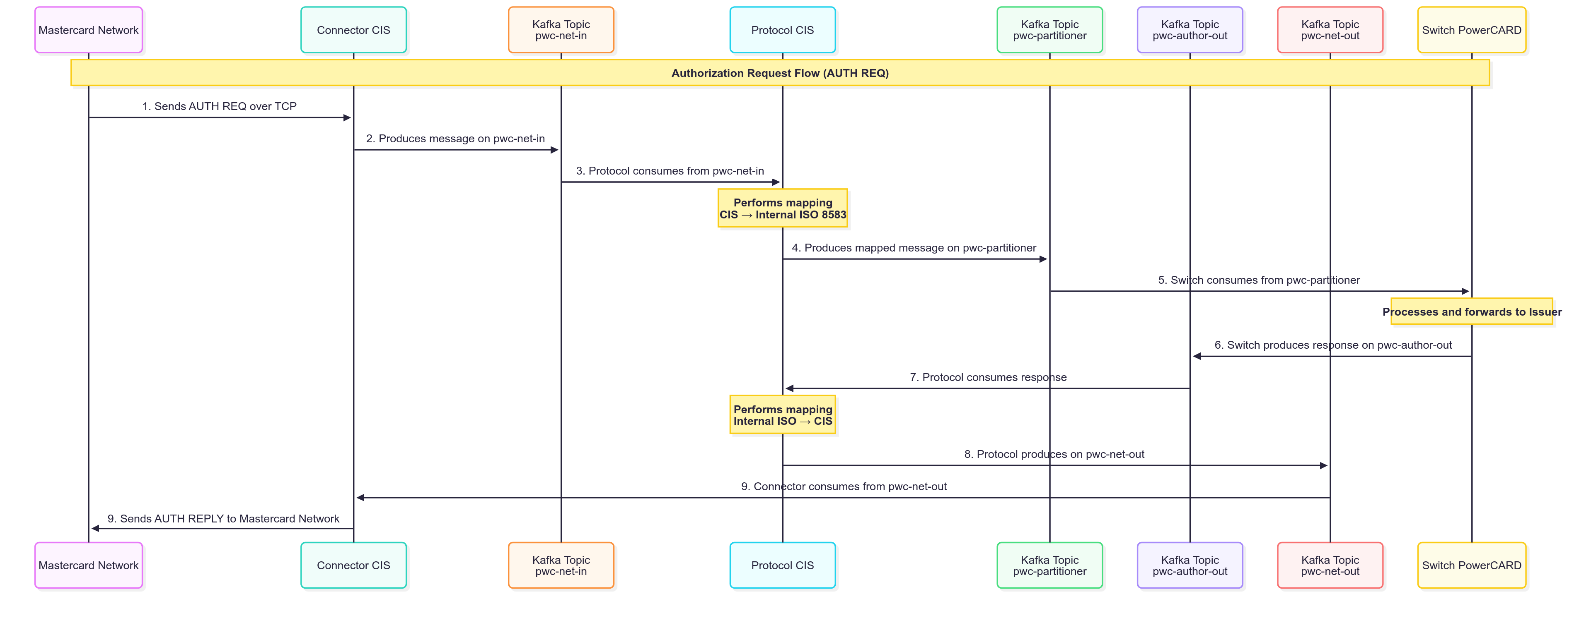
\includegraphics[width=7.21985in,height=2.8089in]{media/image38.png}
\caption{Sequence diagram for autorisation in acquisition}
\label{fig:SDAA}
\end{figure}

\begin{quote}
This diagram shows the complete flow of an authorization request (AUTH
REQ) initiated by Mastercard, typically a 0100 message.

In this scenario, the Mastercard network sends a message to obtain
authorization for a real-time transaction (card payment). The PowerCARD
system acts as a Switch + Issuer.

\textbf{Detailed procedure:}

\textbf{Step 1: Receiving the Mastercard request}

The Mastercard Network sends a CIS authorization message (AUTH REQ) to
the CIS Connector over TCP.

\textbf{Step 2: Kafka Publishing}

The CIS Connector produces the message received on the Kafka topic
pwc-net-in.

This topic is listened to by the CIS Protocol.

\textbf{Step 3: Consume the CIS message}

The CIS Protocol consumes the message from the pwc-net-in topic.

\textbf{Step 4: CIS → ISO 8583 Mapping}

The CIS Protocol converts the message into ISO 8583 internal format:

He then posts this mapped message to the pwc-partitioner topic.

This topic allows the message to be distributed to the correct
partitioner according to the business logic (card, bank, etc.).

\textbf{Step 5: Processing in the PowerCARD Switch}

The PowerCARD Switch consumes the message on pwc-partitioner.

The Switch processes the request:
\end{quote}

\begin{itemize}
\item
  Checking authorization rules
\item
  Balance Check
\item
  Anti-fraud control
\end{itemize}

\begin{quote}
Transmission to the banking core or to the issuer in the event of
outsourcing.

\textbf{Step 6: Production of the response}

The Switch produces the ISO 8583 response (AUTH REPLY) on the
pwc-author-out topic.

\textbf{Step 7: Consume the response}

The CIS Protocol consumes the response from pwc-author-out.

\textbf{Step 8: ISO → CIS Mapping}

The CIS Protocol performs the reverse mapping (ISO → CIS) to reconstruct
the CIS response to return to the Mastercard network.

He produces this response on the pwc-net-out topic.

\textbf{Step 9: Sending the response}

The CIS Connector consumes the message on pwc-net-out and sends the AUTH
REPLY response to the Mastercard network via TCP.
\end{quote}

\begin{quote}
    \textbf{Case authorization issuing:}
\end{quote}

\begin{figure}[H]
\centering
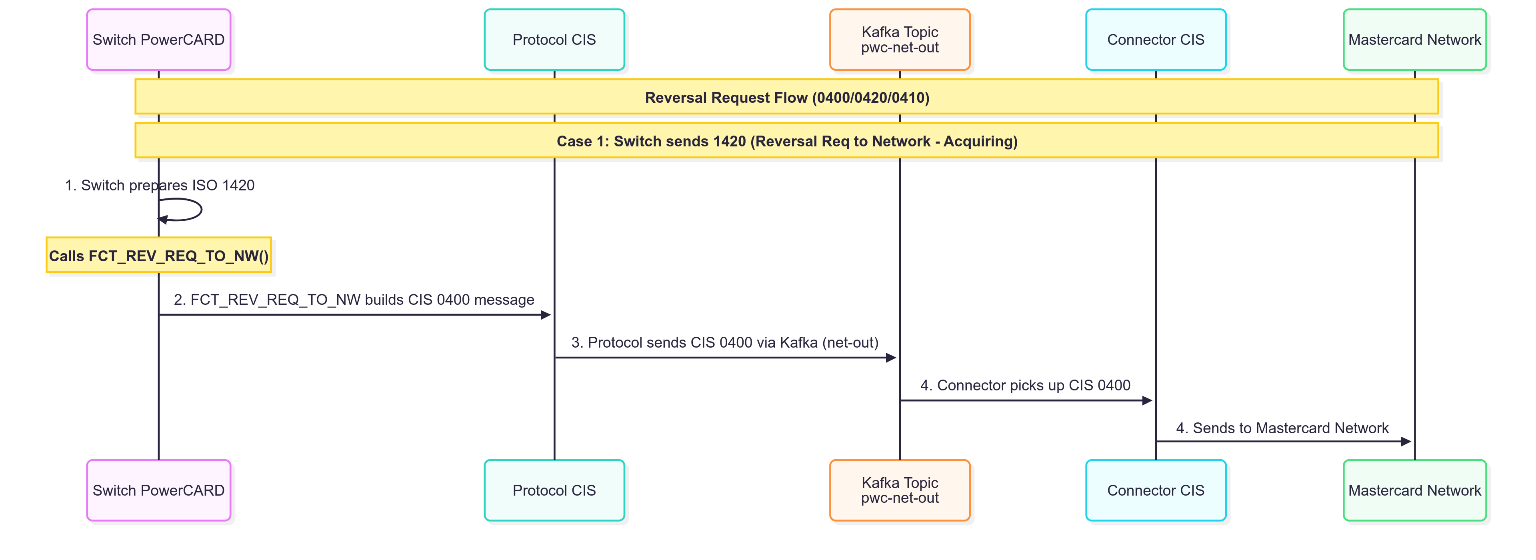
\includegraphics[width=6.97452in,height=2.54278in]{media/image39.png}
\caption{sequence diagram for authorization issuing case}
\label{fig:SDAIC}
\end{figure}

\begin{quote}
This diagram describes the reversal request flow initiated on the
PowerCARD Switch side for an acquiring mode transaction.

Typically, this is an ISO 1420 → message transformed into CIS 0400 sent
to Mastercard Network to signal a reversal of a previous transaction
(example: cancellation of a payment).

\textbf{Detailed procedure:}

\textbf{Step 1: Preparation of ISO 1420}

The PowerCARD Switch prepares an ISO 1420 message (reversal request).

This message is generated in response to internal logic (timeout,
cancellation, confirmation failure, etc.).

\textbf{Step 2: CIS 0400 Construction}

Constructs a message in CIS 0400 format (format expected by the
Mastercard network).

This conversion follows business rules (ISO → CIS field mapping).

\textbf{Step 3: Send Kafka}

The CIS Protocol publishes the CIS 0400 message to the Kafka topic:
pwc-net-out

This topic allows routing to the CIS Connector.

\textbf{Step 4: Send to the Mastercard network}

The CIS Connector consumes the CIS 0400 message from pwc-net-out → then
sends it via TCP/IP to the Mastercard network.
\end{quote}
\clearpage
\begin{quote}
\textbf{Reversal issuing case:}  
\end{quote}

\begin{figure}[H]
\centering
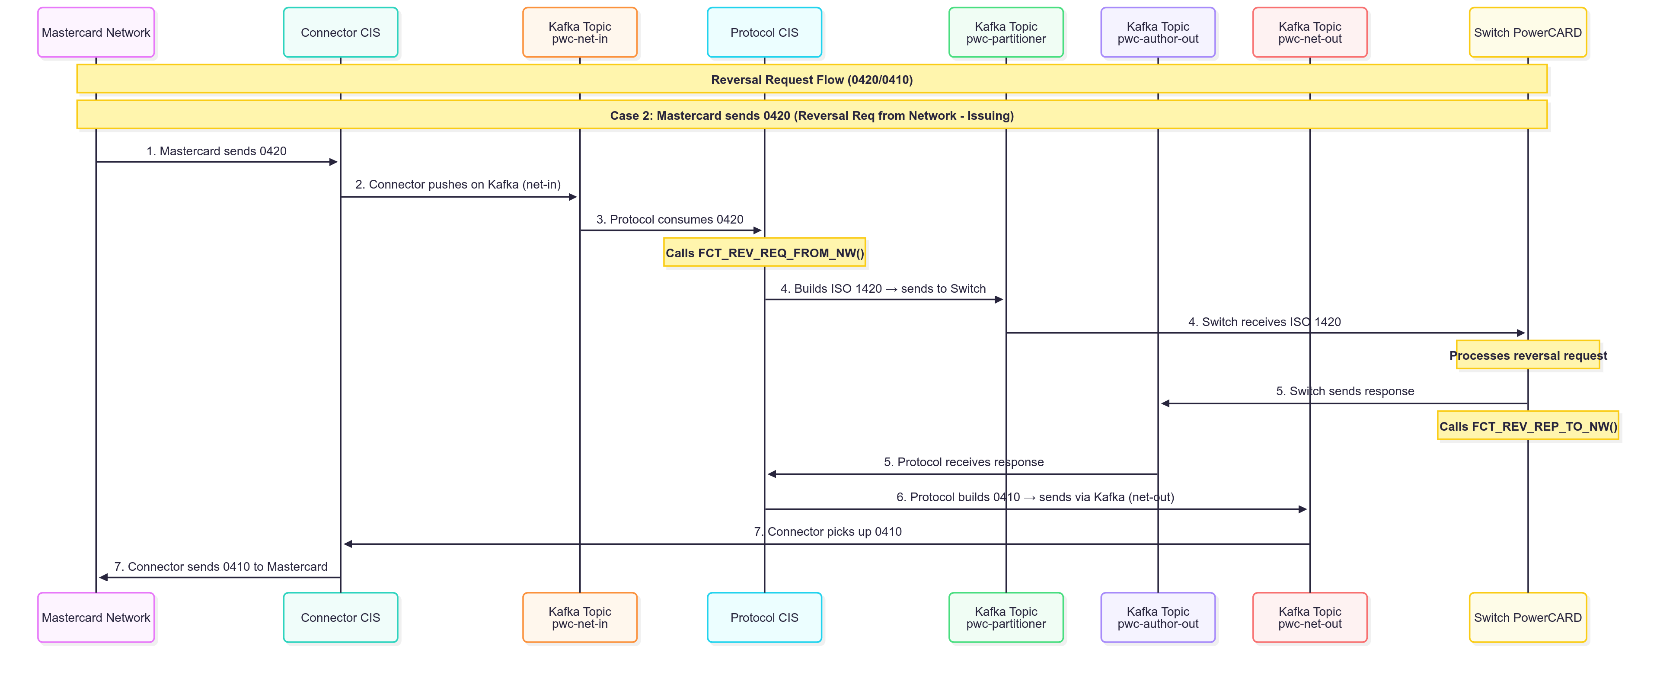
\includegraphics[width=6.95813in,height=2.23377in]{media/image40.png}
\caption{Sequence Diagram of the reversal acquisition}
\label{fig:SDRA}
\end{figure}
\begin{quote}
This diagram illustrates the processing of a reversal request initiated
by the Mastercard network to the PowerCARD Switch, in issuing mode.

Typically, the Mastercard network wants to cancel a transaction, so it
sends a 0420 message to the system.

\textbf{Step 1: Send by Mastercard}

The Mastercard network sends a 0420 (Reversal Request) message to the
system.

\textbf{Step 2: Kafka Publishing}

The CIS Connector receives the 0420 and publishes it on the Kafka topic:

pwc-net-in

\textbf{Step 3: Consumption by protocol}

The CIS Protocol consumes this 0420 message.

\textbf{Step 4: ISO 1420 Construction}

Constructed from an ISO 1420 message

\textbf{Step 5: Reception and processing}

The PowerCARD Switch receives the ISO 1420, processes the reversal
request, and then prepares a response.

\textbf{Step 6: Construction 0410}

The CIS Protocol receives this ISO response, constructs a CIS 0410
(Reversal Response) message, and publishes it to the Kafka topic:

pwc-net-out

\textbf{Step 7: Transmission to Mastercard}

The CIS Connector consumes the 0410 message from Kafka, and sends it to
the Mastercard network in response to the initial request.
\end{quote}

\begin{quote}
\textbf{Advice acquiring :}
\end{quote}

\begin{figure}[H]
\centering
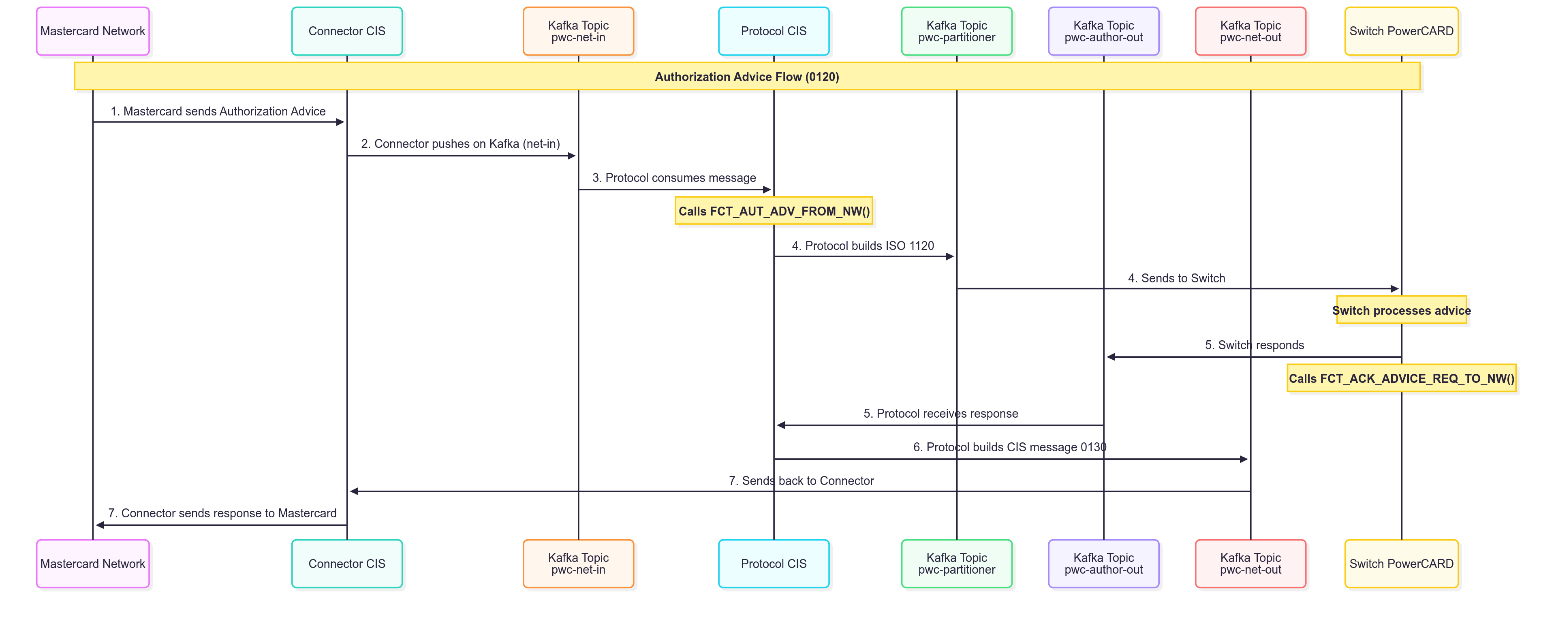
\includegraphics[width=7.05923in,height=2.81006in]{media/image41.png}
\caption{sequence diagram of advice acquisition}
\label{fig:SDAA}
\end{figure}

\begin{quote}
This diagram describes the Authorization Advice (0120) message flow
initiated by the Mastercard network, in acquiring mode. This type of
message is used to notify the Switch that a transaction has been
authorized or regularized (e.g. offline transactions, correction,
supplement).

\textbf{Step 1: Receiving 0120}\\
The Mastercard network sends an Authorization Advice 0120 message via
TCP to the CIS Connector.

\textbf{Step 2: Injection into Kafka}\\
The CIS Connector publishes this message 0120 to the Kafka topic
pwc-net-in for processing.

\textbf{Step 3: Processing by the CIS Protocol}\\
The CIS Protocol consumes the 0120 message and calls the function which
is responsible for performing the reversal logic in acquisition.

\textbf{Step 4: Convert to ISO 1120}\\
The protocol converts the message into ISO 1120 format, the format
expected by the PowerCARD Switch, and sends it to the Switch.

\textbf{Step 5: Processing by the Switch}\\
The PowerCARD Switch receives the ISO 1120 message and processes the
authorization advice (update of databases, regularization, etc.).

\textbf{Step 6: Construction of the 0130}\\
The CIS Protocol constructs the CIS 0130 message (response to Advice)
and publishes it to the Kafka topic pwc-net-out.

\textbf{Step 7: Return to Mastercard}\\
The CIS Connector consumes the 0130 message and transmits it to the
Mastercard network, finalizing the advice processing.
\end{quote}

\begin{quote}
\textbf{File upload issuing case:}
\end{quote}

\begin{figure}[H]
\centering
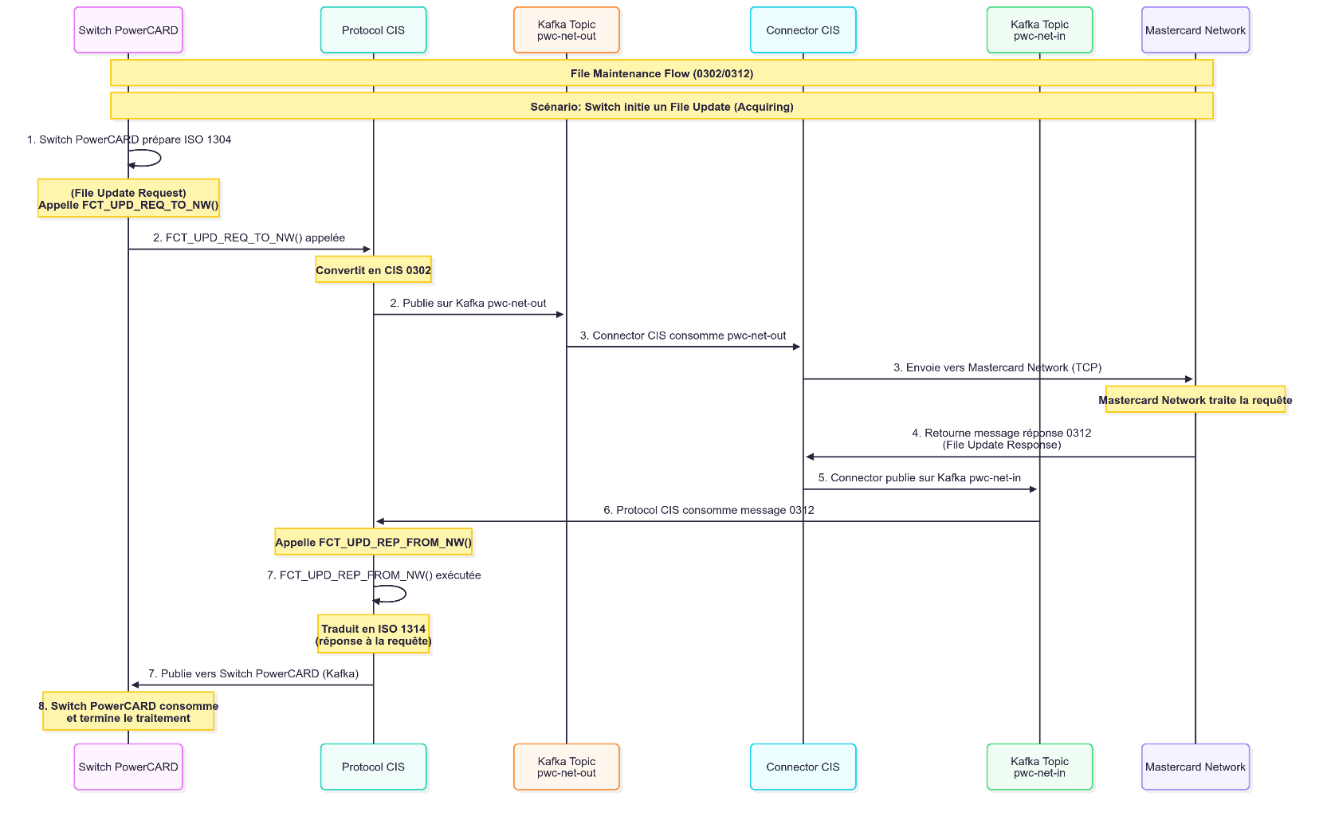
\includegraphics[width=6in,height=1\textheight,keepaspectratio]{media/image42.png}
\caption{sequence diagram of the emission file upload}
\label{fig:SDEA}
\end{figure}

\begin{quote}
This diagram describes the Authorization Advice message flow in issuing
mode, initiated by the Mastercard network. This is a CIS 0120 message
sent by Mastercard → which will be transformed into an ISO 1120 message
to the PowerCARD Switch, to inform of an authorized operation
(authorization advice, non-blocking).

\textbf{Step 1: Receiving message 0120}\\
The Mastercard network sends an Authorization Advice 0120 message via
TCP to the CIS Connector.

\textbf{Step 2: Injection into Kafka}\\
The CIS Connector publishes this message to the Kafka topic pwc-net-in,
for processing by the protocol.

\textbf{Step 3: Processing by the CIS Protocol}\\
The CIS Protocol consumes message 0120. It calls the function which:
\end{quote}

\begin{itemize}
\item
  \begin{quote}
  Converts the message to ISO 1120
  \end{quote}
\item
  \begin{quote}
  Inserts the original into the temporary table so that the ACK can be
  processed later.
  \end{quote}
\end{itemize}

\begin{quote}
The ISO 1120 message is sent to the PowerCARD Switch.

\textbf{Step 4: Processing in the Switch}\\
The PowerCARD Switch receives the ISO 1120 message and processes the
advice (internal update, log, statistics, etc.). The Switch then returns
an ISO 1130 or equivalent response message (indicating success or other
status).

\textbf{Step 5: Preparing the ACK}\\
The CIS Protocol receives this response, calls a function which:
\end{quote}

\begin{itemize}
\item
  \begin{quote}
  Retrieves the original query.
  \end{quote}
\item
  \begin{quote}
  Constructs the CIS 0130 response.
  \end{quote}
\end{itemize}

\begin{quote}
\textbf{Step 6: Return to Mastercard}\\
The CIS Connector then forwards this CIS 0130 message to the Mastercard
network, finalizing the advice flow.
\end{quote}

\begin{quote}
\textbf{File upload in acquisition:}
\end{quote}

\begin{figure}[H]
\centering
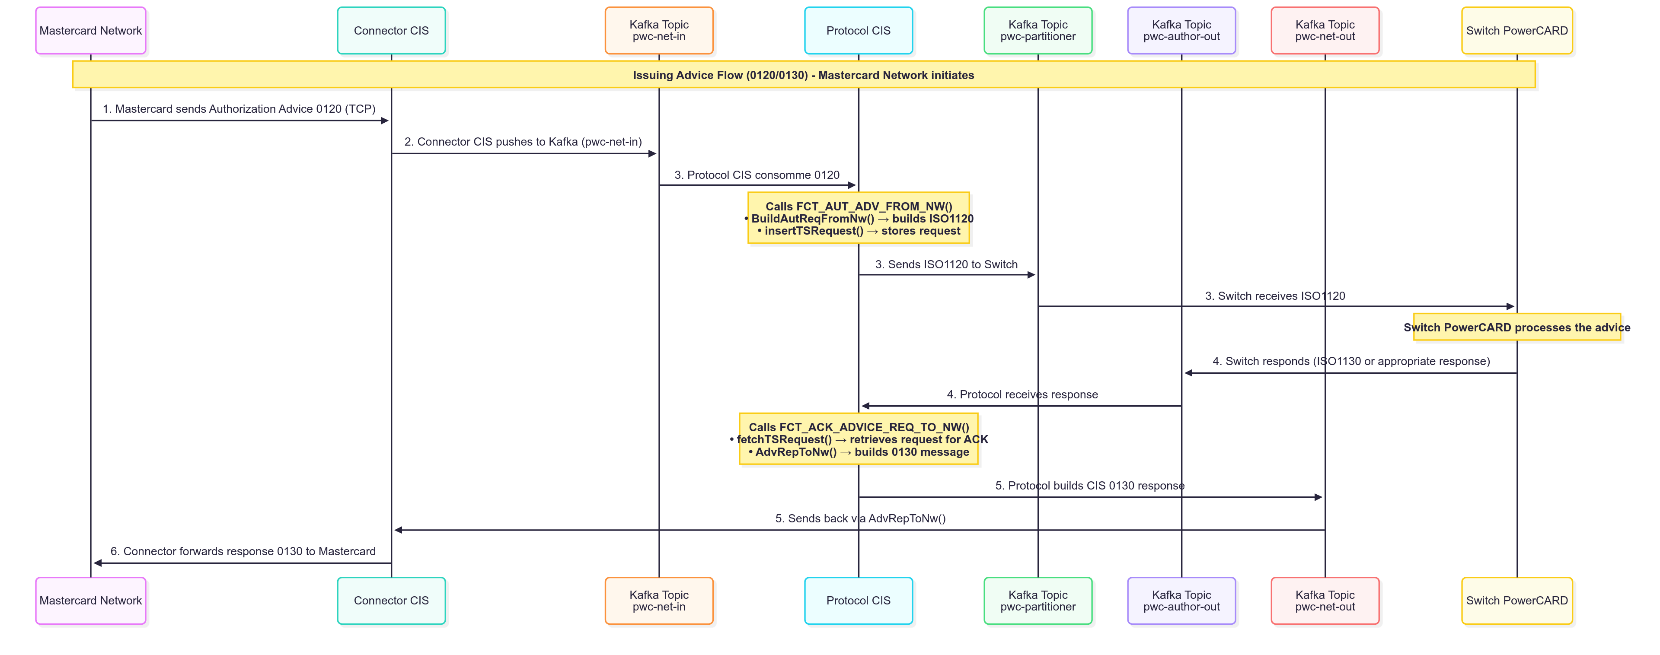
\includegraphics[width=\textwidth,height=1\textheight,keepaspectratio]{media/image43.png}
\caption{Sequence diagram in the acquisition of file upload}
\label{fig:FUSD}
\end{figure}

\begin{quote}
This diagram describes the file maintenance request flow initiated on
the PowerCARD Switch side in acquiring mode. This is typically an ISO
1304 message (file update request) → transformed into a CIS 0302 message
sent to the Mastercard network to perform an update on a remote file
(addition, modification, deletion or information request).

\textbf{Detailed procedure:}

\textbf{Step 1: Preparation of ISO 1304}\\
The PowerCARD Switch prepares an ISO 1304 message representing a file
update request. This message is constructed based on the operations
requested by the back office or management system.

\textbf{Step 2: CIS 0302 Construction}\\
Constructs a message in CIS 0302 format (format expected by the
Mastercard network). This conversion respects the mapping rules between
ISO and CIS fields.

\textbf{Step 3: Kafka Publishing}\\
The CIS Protocol publishes the CIS 0302 message on the Kafka topic:
pwc-net-out. This topic is used to transmit the message to the CIS
Connector.

\textbf{Step 4: Send to Mastercard}\\
The CIS Connector consumes the 0302 message from pwc-net-out and sends
it via TCP/IP to the Mastercard network.

\textbf{Step 5: Return response 0312}\\
The Mastercard network processes the file update request and returns a
CIS 0312 response (file update response). The CIS Connector receives
this response and publishes it to Kafka: pwc-net-in.

\textbf{Step 6: Processing response 0312}\\
CIS Protocol consumes response 0312 from pwc-net-in

\textbf{Step 7: Convert to ISO 1314}\\
Convection of the CIS response into an ISO 1314 message (response to the
file update request), and publishes it to Kafka for the Switch.

\textbf{Step 8: Finalization}\\
The PowerCARD Switch consumes the ISO 1314 message and completes
processing the update request.
\end{quote}
\clearpage

\subsubsubsection{Activity diagram :}
\begin{quote}
\textbf{Request for authorization for acquisition :}
\end{quote}

\begin{figure}[H]
\centering
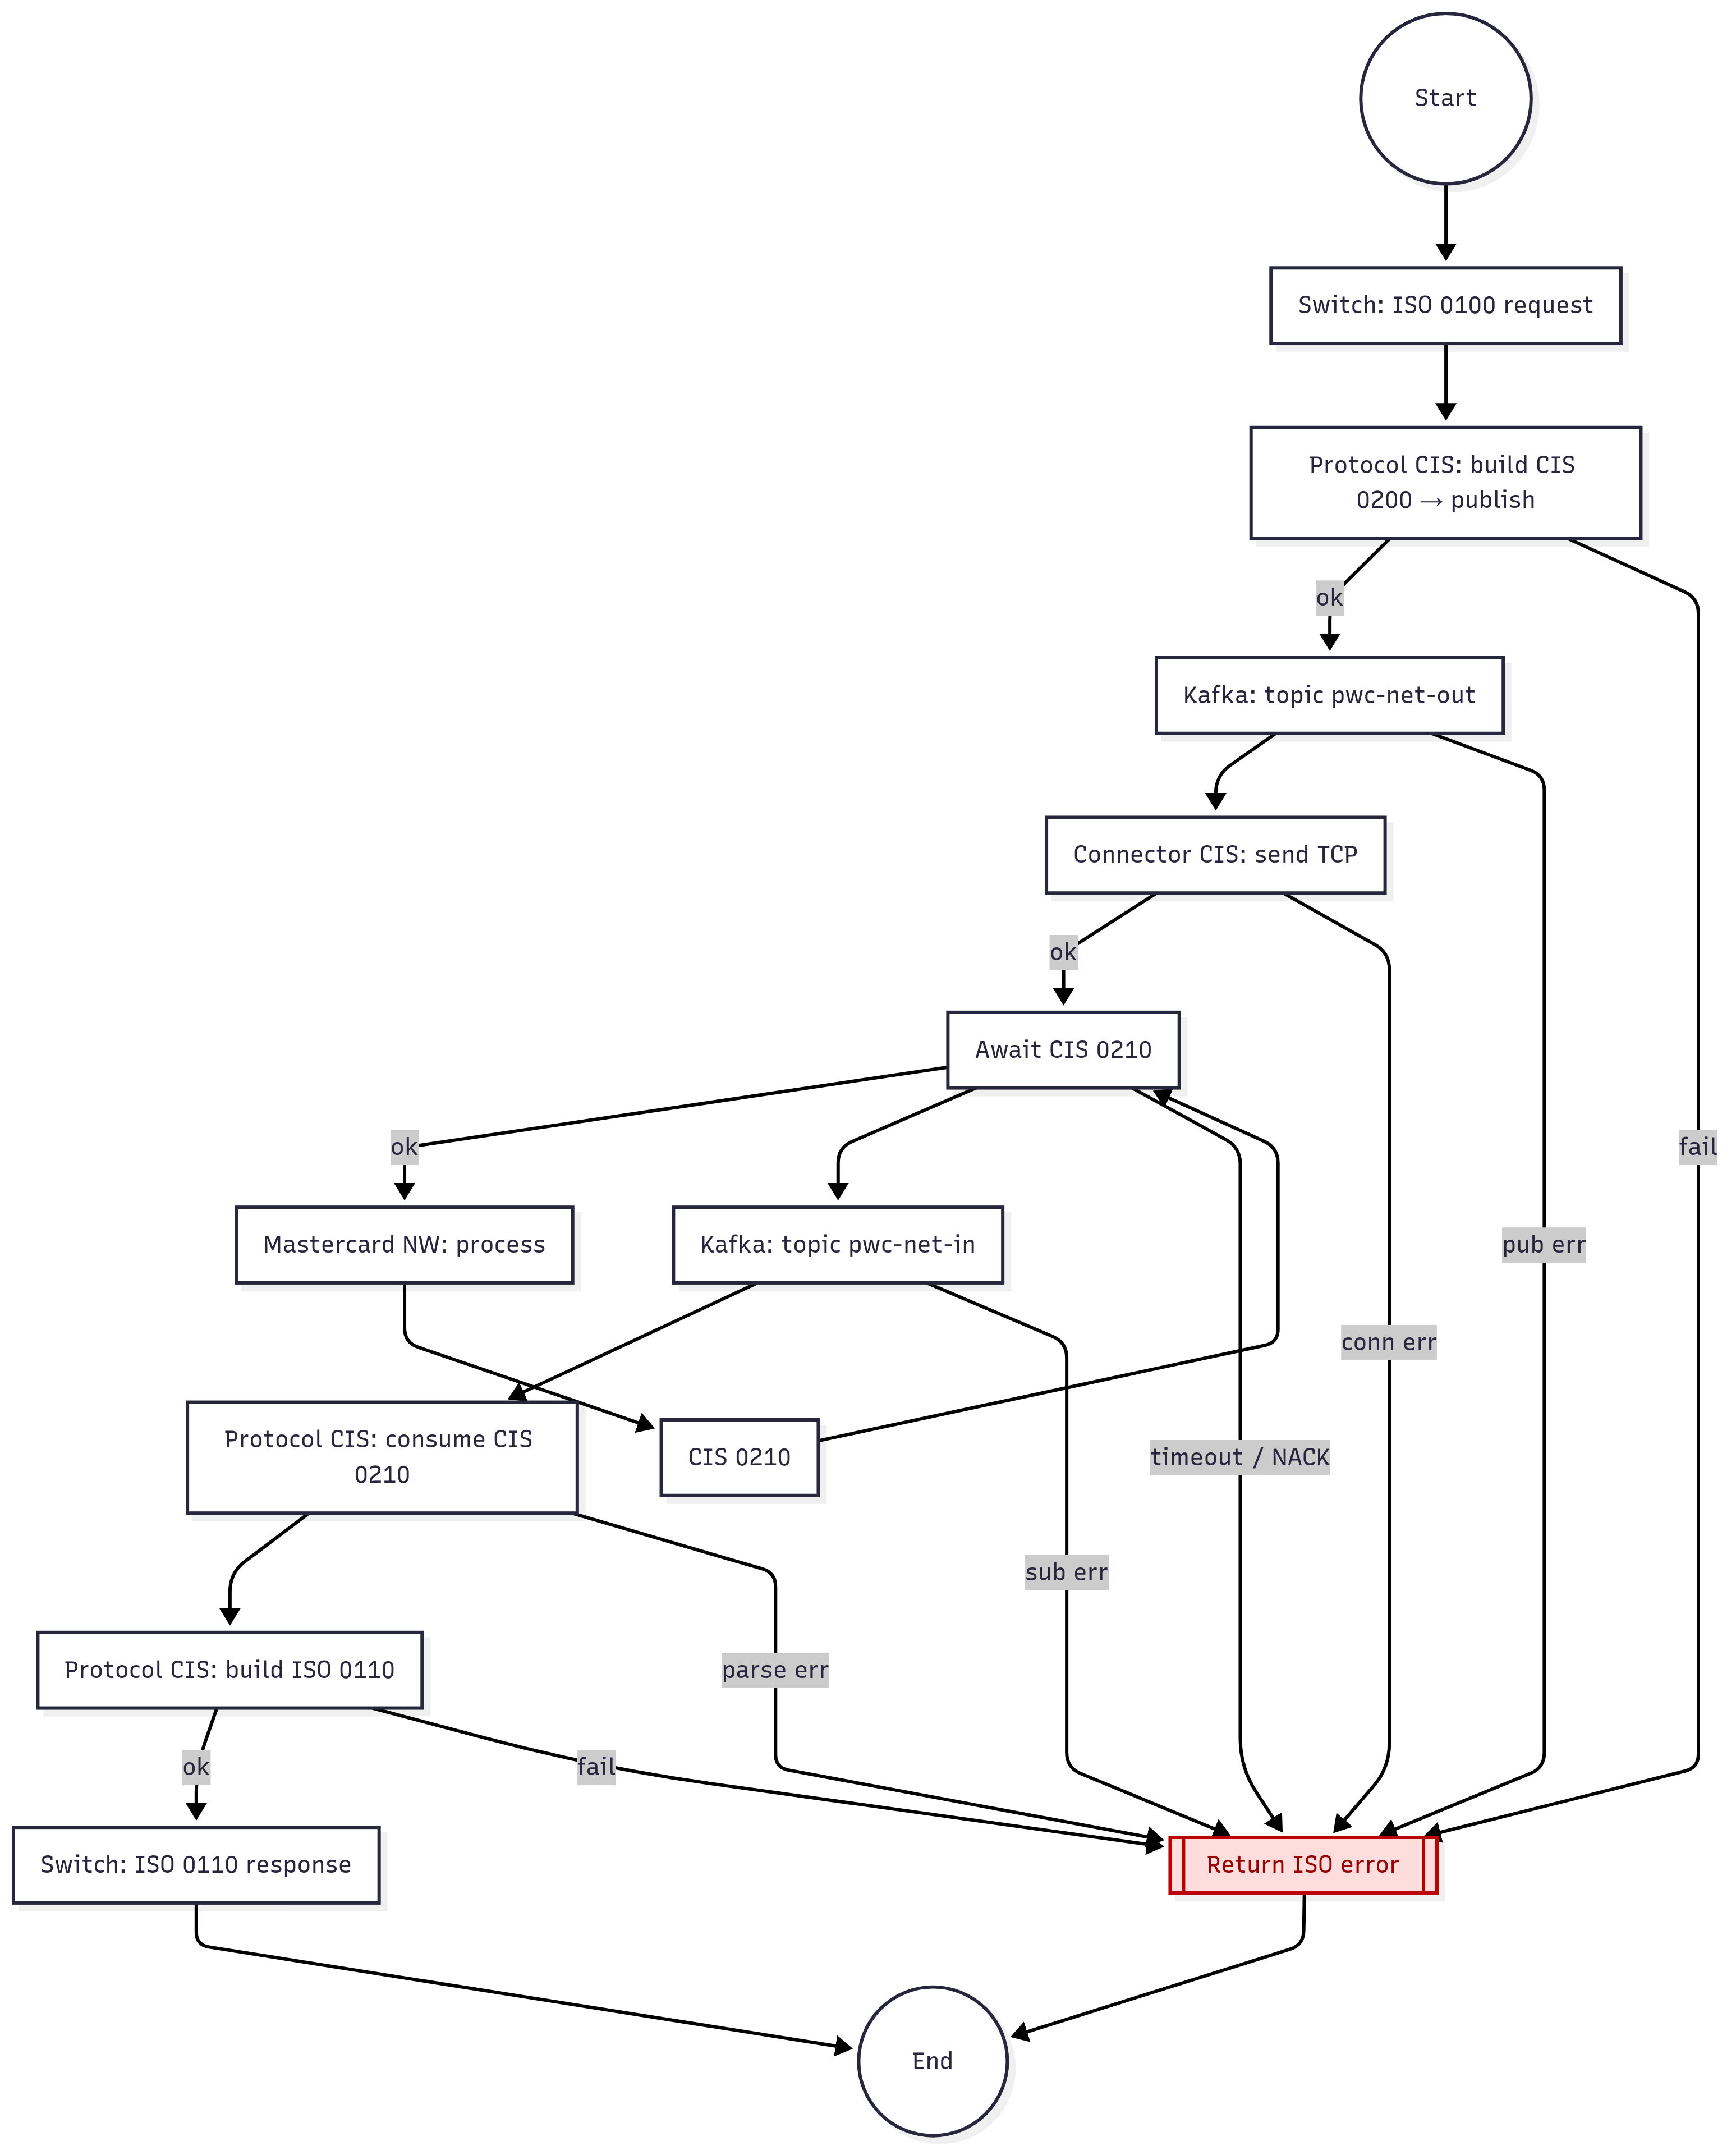
\includegraphics[width=\textwidth,height=1\textheight,keepaspectratio]{media/acq-auth-req-activity.png}
\caption{Activity Diagram Acquisition Authorization Request}
\label{fig:ADAAR}
\end{figure}

\begin{quote}
The activity diagram depicts the full life-cycle of an acquiring-side authorisation, beginning with the Switch emitting an ISO 0100 request and ending with either a normal ISO 0110 reply or an error response. After the Switch submits the 0100, the Protocol CIS module translates it into a CIS 0200 message and publishes that frame on the pwc-net-out Kafka topic. A Connector CIS service consumes the record, conveys it to Mastercard over a TCP session, and the system enters a wait state for the remote CIS 0210 reply. When the 0210 arrives it is republished on pwc-net-in, re-consumed by Protocol CIS, reformatted into ISO 0110, and forwarded to the Switch for delivery to the business application—thus completing the positive path. Every critical hop carries its own exception branch: a Kafka publish failure (pub err), TCP transport failure (conn err), subscription failure on the inbound topic (sub err), message-parsing anomaly (parse err), or network timeout/negative acknowledgement (timeout / NACK). Whichever of these contingencies is triggered, control converges on a single “Return ISO error” action, ensuring that the Switch receives a syntactically valid but negative ISO response (typically RC 06, 91 or 96) while operational logs and alerts capture the root cause. Consequently, the diagram highlights both the nominal processing flow and the error-handling fabric that preserves transactional integrity under adverse conditions.
\end{quote}
\clearpage

\begin{quote}
\textbf{Request for Issuing Authorization:}
\end{quote}

\begin{figure}[H]
\centering
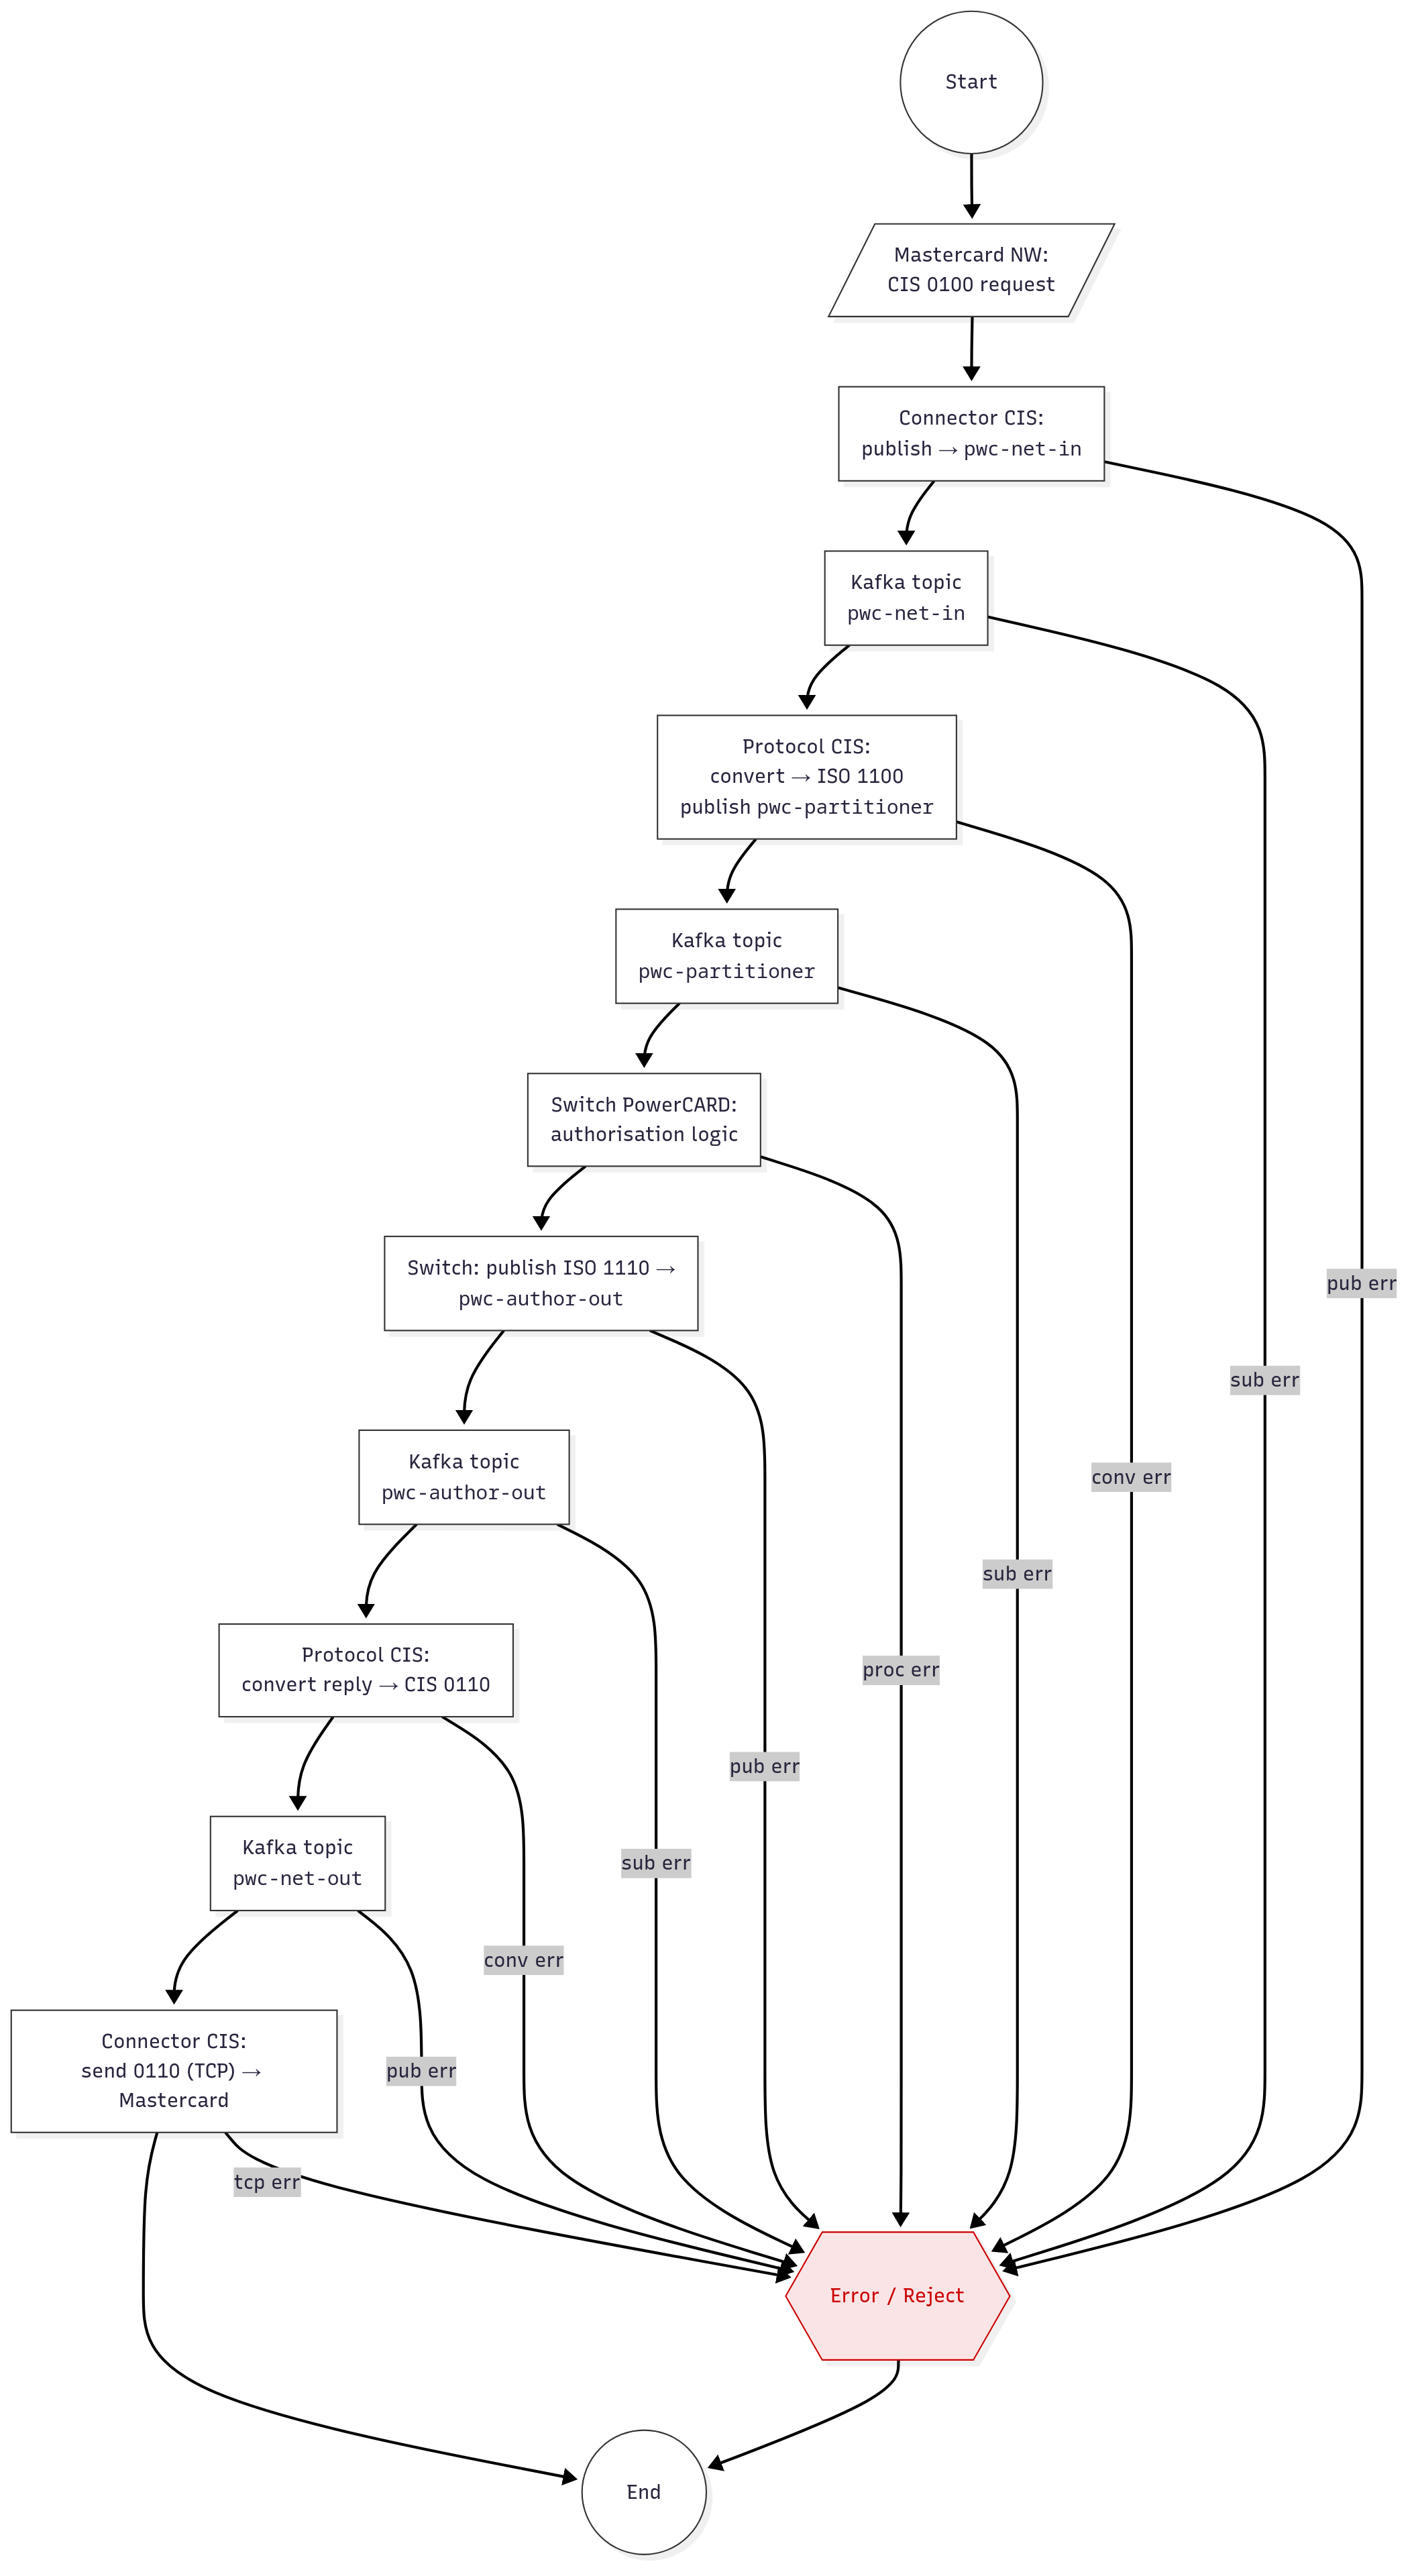
\includegraphics[width=\textwidth,height=0.85\textheight,keepaspectratio]{media/iss-auth-req-activity.png}
\caption{Activity Diagram Schema Authorization Request Issuing}
\label{fig:ADSARI}
\end{figure}
\clearpage

\begin{quote}
This activity diagram captures the end-to-end life-cycle of an issuing-side authorisation request originating from Mastercard’s CIS network (0100).
The flow starts once the 0100 frame reaches the PowerCARD ecosystem: the Connector component ingests the message and publishes it to the pwc-net-in Kafka topic. Protocol CIS immediately consumes the record, performs a rigorous CIS→ISO conversion (producing an ISO 1100), and republishes the transformed message to pwc-partitioner. The Switch’s authorisation engine then executes all business and risk checks; upon success it emits an ISO 1110 reply to pwc-author-out.
The reply traverses the reverse path: Protocol CIS converts ISO 1110 back to CIS 0110, places it on pwc-net-out, and the Connector delivers the TCP frame to Mastercard.
At every asynchronous hop—publish, subscribe, conversion, processing, and final TCP delivery—dedicated error guards are shown (labels such as pub err, sub err, conv err, proc err, tcp err). Any of these anomalies triggers an immediate divergence to the red Error / Reject gateway, enforcing a single, auditable exit for negative outcomes before the diagram terminates. The structure therefore emphasises both the nominal “happy path” and the consolidated error-handling strategy that guarantees determinism and observability across the Kafka-centric micro-pipeline.
\end{quote}
\clearpage


\begin{quote}
\textbf{Acquisition reversal acquisition:}    
\end{quote}
    
\begin{figure}[H]
\centering
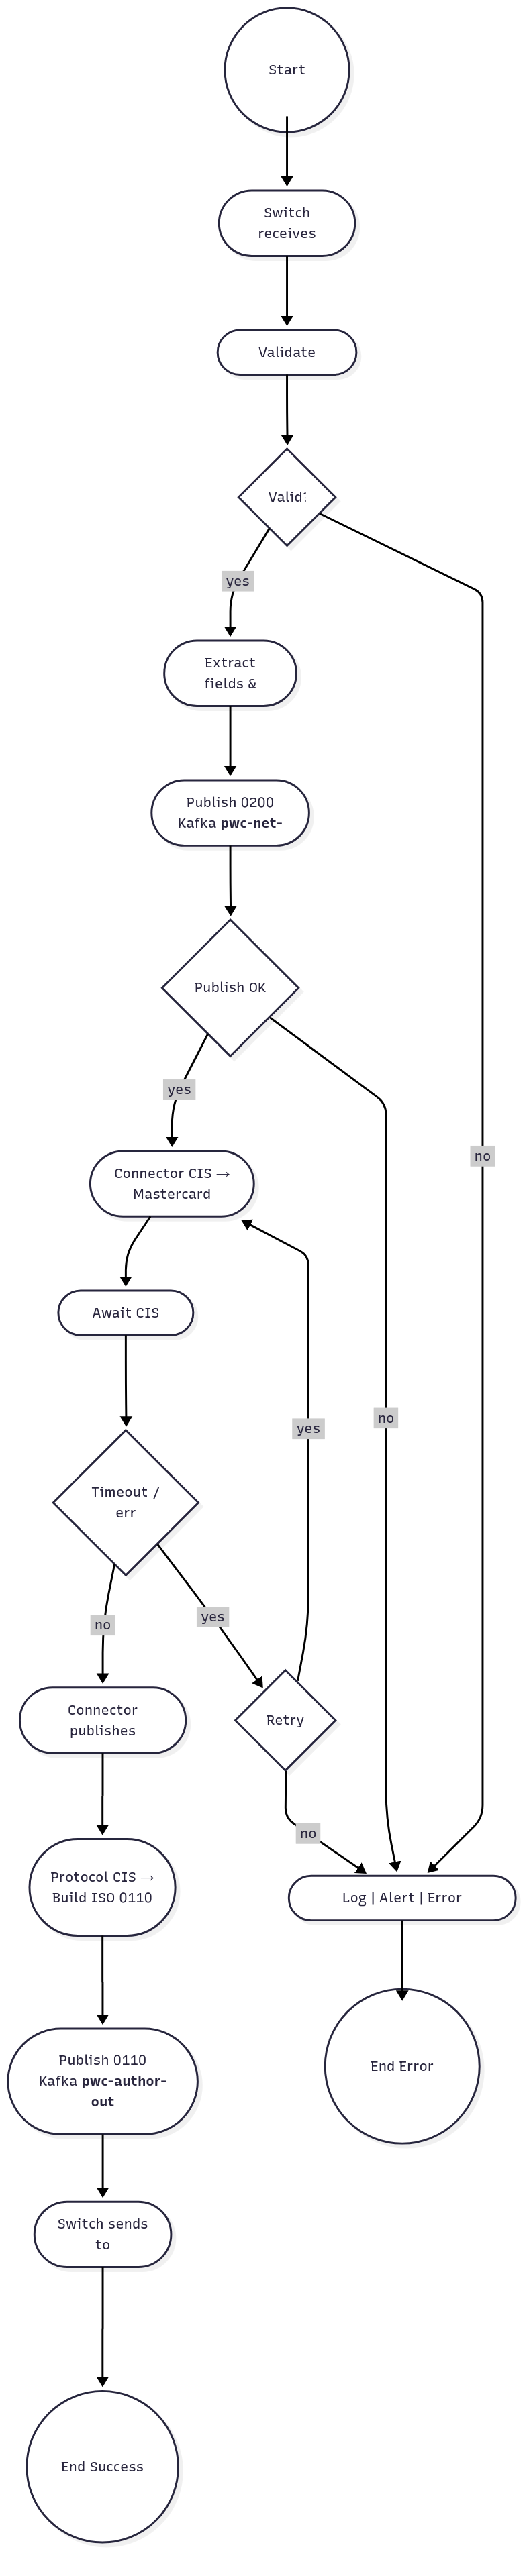
\includegraphics[width=\textwidth,height=0.85\textheight,keepaspectratio]{media/acq-rev-auth-req.png}
\caption{Activity Diagram Reversal Acquisition}
\label{fig:ADRA}
\end{figure}
\clearpage

\begin{quote}
The activity chart depicts the life-cycle of an acquiring authorisation request that originates inside the Switch and is routed to Mastercard.
The flow begins when the Switch receives an ISO 0100 message and performs a full syntactic and business-rule validation.
\begin{itemize}
\item If the message fails validation the run terminates at a central Log | Alert | Error action.
\item Otherwise, the Switch extracts the required data elements, builds a CIS 0200, and attempts to publish it to the pwc-net-out Kafka topic.
A first decision node checks whether the publication succeeded. Any failure (e.g., broker unavailability) leads directly to the error-handling action mentioned above. If the record is accepted, the Connector forwards the CIS 0200 to Mastercard over TCP and the system waits for a network reply.
While waiting, a second decision evaluates whether a timeout or transport error has occurred.
\item On such an event, control moves to a Retry gate: if retries are still permitted the logic loops back to the publication step; once the retry budget is exhausted the execution proceeds to the error-handling action.
\item When a CIS response is received in time, the Connector publishes it to Kafka; Protocol CIS converts the payload to an ISO 0110, publishes that reply to pwc-author-out, and the Switch forwards the response to the requesting application.
\end{itemize}
Successful completion of these steps reaches the End Success terminator. All abnormal situations—validation failure, publication fault, connector error, unreachable network, or exhausted retries—merge at the Log | Alert | Error node before reaching the End Error terminator, guaranteeing consistent auditing and monitoring for every exception.

\end{quote}
\clearpage

\begin{quote}
\textbf{Reversal of issue issuing:}
\end{quote}

\begin{figure}[H]
\centering
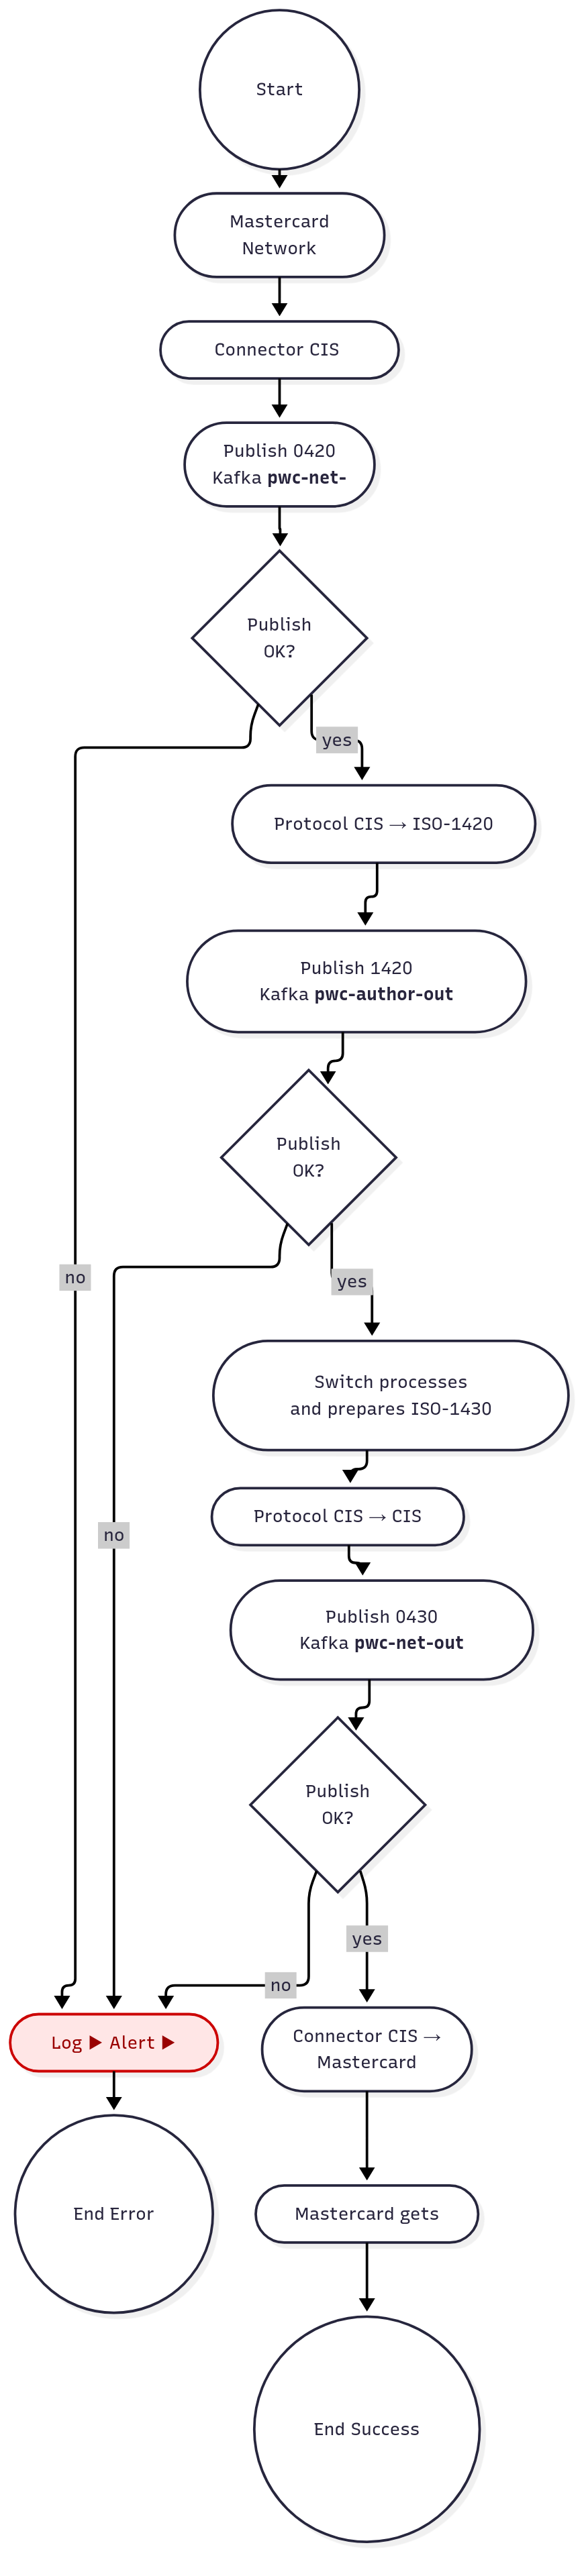
\includegraphics[width=\textwidth,height=0.85\textheight,keepaspectratio]{media/iss-rev-auth-req.png}
\caption{Activity Diagram  Reversal Issuing}
\label{fig:ACD}
\end{figure}
\clearpage

\begin{quote}
This flow describes how a reversal initiated by Mastercard (CIS 0420) propagates through the PowerCARD platform, is transformed, processed, and ultimately returned to the network, together with the points at which operational safeguards intervene if something goes wrong.
The sequence starts when Mastercard delivers a CIS 0420 reversal message. The Connector CIS ingests the frame and tries to publish it to the inbound network topic pwc-net-in. Publication is immediately verified; if the broker rejects the record the flow is diverted to a unified Log → Alert → End Error branch, ensuring that upstream systems are notified and no orphaned reversal continues.
When the broker accepts the record, Protocol CIS converts the payload to ISO 1420 and places it on pwc-author-out for the Switch. A second publication check safeguards this step in the same way.
The Switch PowerCARD retrieves the ISO 1420, locates the original authorisation, performs the reversal logic, and assembles an ISO 1430 response. That response is sent back to Protocol CIS, converted to CIS 0430, and queued on pwc-net-out. A third publication gate again determines whether the process can continue or must fall back to the error channel.
If the final broker write succeeds, the Connector CIS transmits the CIS 0430 over TCP to Mastercard. Receipt by the network closes the transaction and the diagram converges on End Success. At each broker interaction a “publish OK?” decision diamond routes failures to the same consolidated logging and alert mechanism, guaranteeing consistent error capture and termination across all stages.

\end{quote}
\clearpage

\begin{quote}
\textbf{Authorization Advice:}
\end{quote}

\begin{figure}[H]
\centering
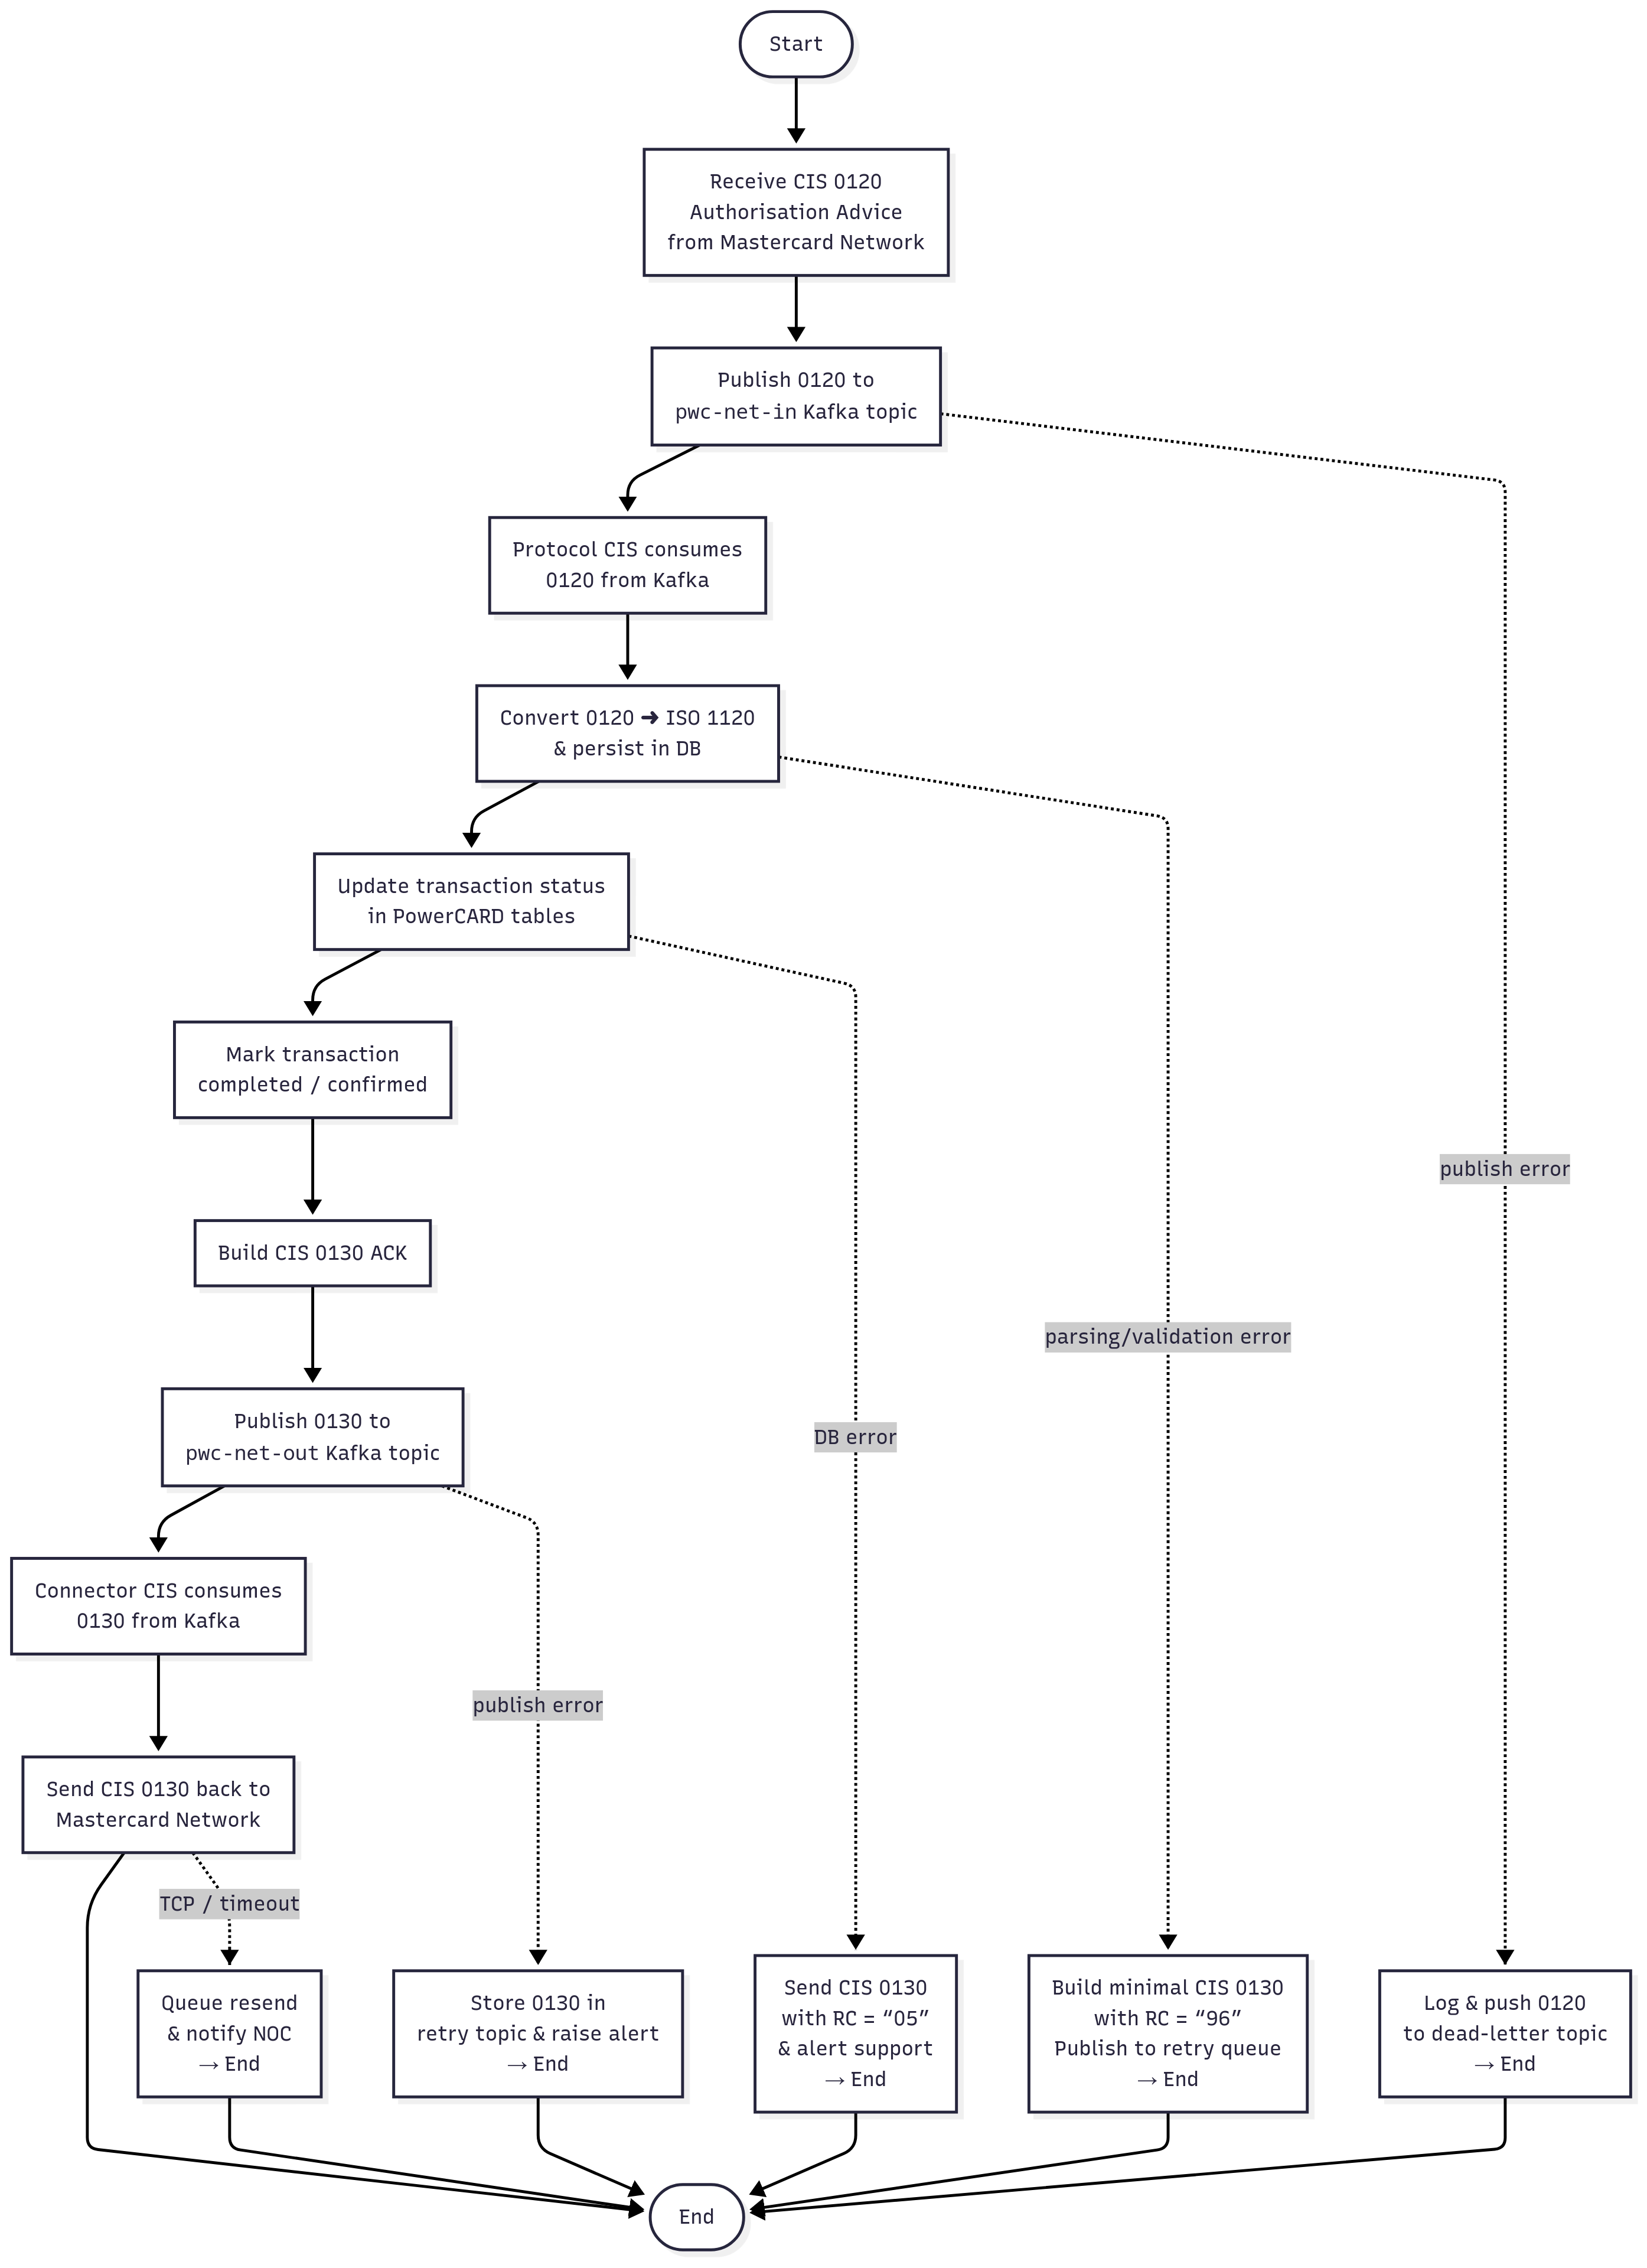
\includegraphics[width=\textwidth,height=0.85\textheight,keepaspectratio]{media/advice-auth-activity.png}
\caption{Activity Diagram Advice }
\label{fig:}
\end{figure}
\clearpage

\begin{quote}
The diagram details the life-cycle of an incoming Mastercard authorisation advice (CIS 0120) that must be acknowledged by PowerCARD with a CIS 0130 and highlights the safeguards that protect each processing stage.
1.	Network ingress : A CIS 0120 is received over TCP, forwarded by the Connector to the inbound Kafka topic pwc-net-in, and immediately consumed by Protocol CIS.
2.	Normal processing : Protocol CIS parses the frame, converts it to ISO 1120, persists the ISO image, and triggers a status update in the PowerCARD transaction tables. When the record is flagged completed/confirmed, the module assembles a CIS 0130 acknowledgement and publishes it on the outbound topic pwc-net-out. The Connector subsequently relays the 0130 to Mastercard, ending the flow.
3.	Protective branches :
\begin{itemize}
\item Parsing / validation failure → a minimal CIS 0130 with response code “96” (system malfunction) is published to a retry queue.
\item Database error while updating tables → a CIS 0130 with response code “05” (do not honour) is returned and support is alerted.
\item Kafka publish error for the outbound 0130 → the message is written to a retry topic for later replay and operations are notified.
\item Publish error for the inbound 0120 → the original advice is logged and routed to a dead-letter topic to guarantee traceability.
\item TCP timeout when sending 0130 back to Mastercard → the message is queued for automatic resend and the NOC is informed.
Solid lines show the principal sequence; dotted lines branch to the above contingencies. Every error path converges on a controlled termination, ensuring that no advice is lost and that support teams receive the context required to intervene.
\end{itemize}

\end{quote}
\clearpage

\begin{quote}
\textbf{File upload :}
\end{quote}

\begin{figure}[H]
\centering
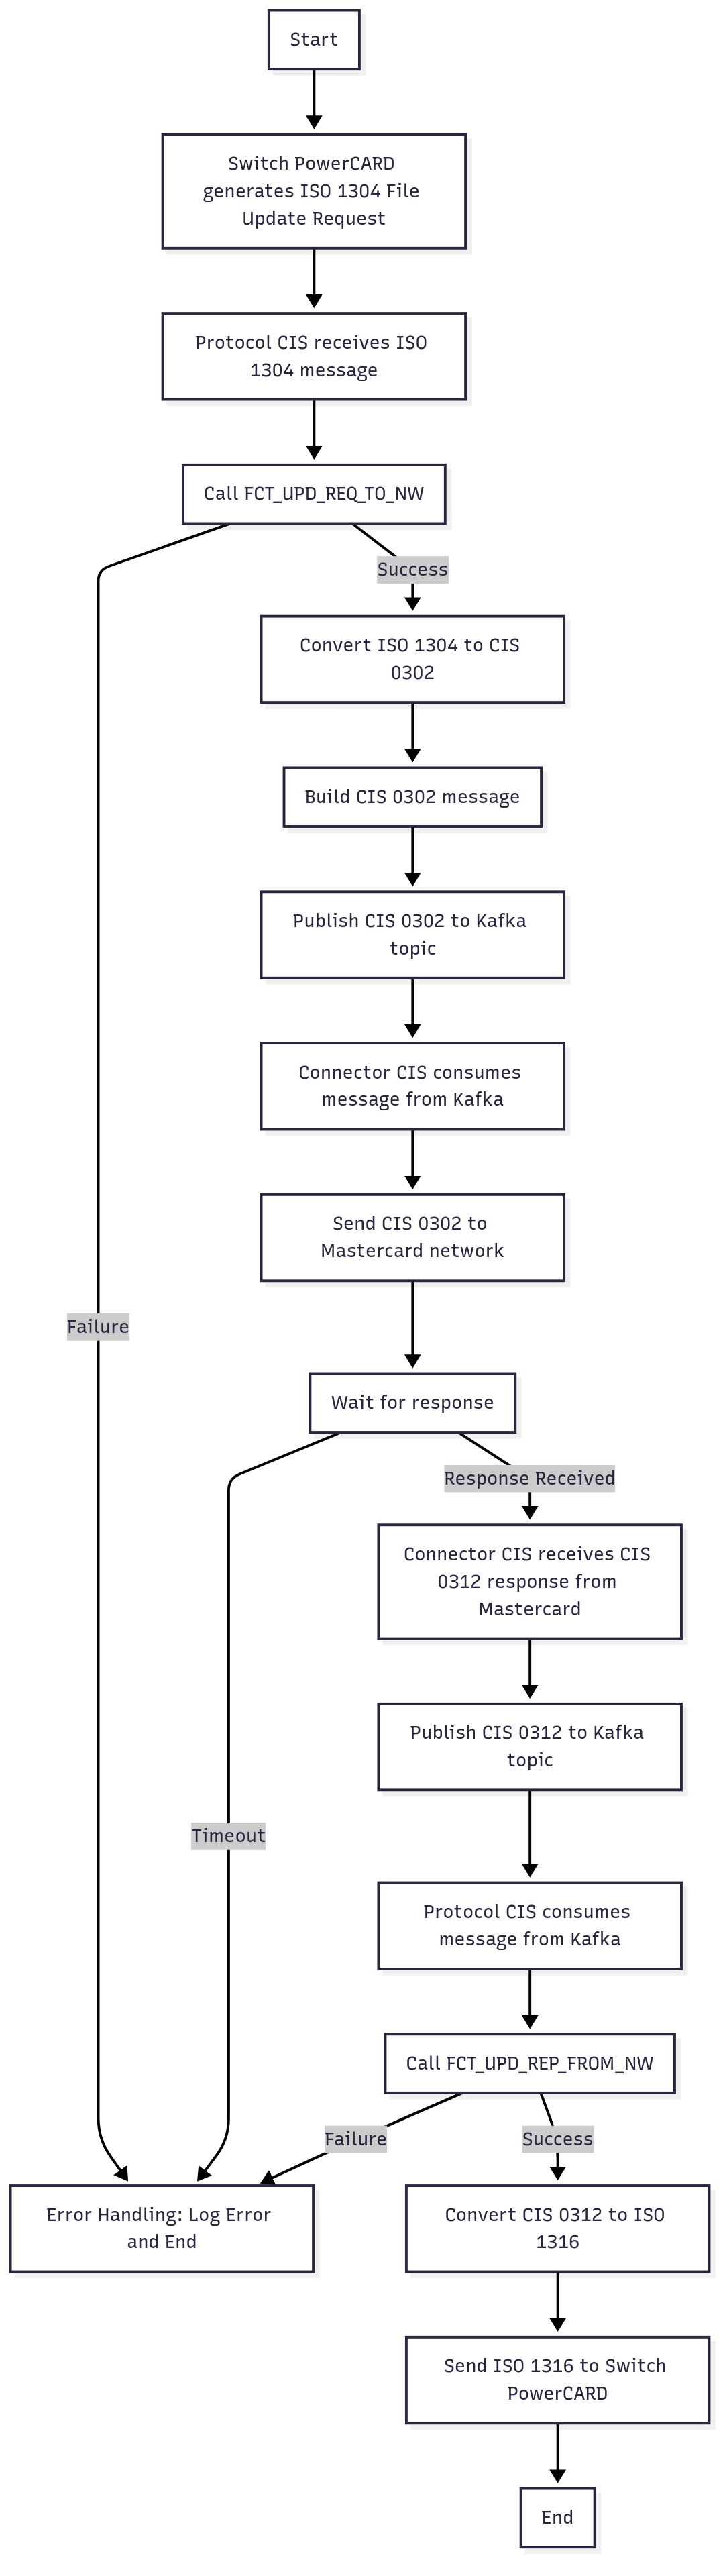
\includegraphics[width=\textwidth,height=0.85\textheight,keepaspectratio]{media/file-upload-activity.png}
\caption{Activity Diagram  file upload}
\label{fig:DFileUp}
\end{figure}

\clearpage

\begin{quote}
The flow describes a file upload update initiated by the Switch using ISO 1304, and completed only once Mastercard’s 0312 reply is translated back to ISO 1316.

After the Switch initiates the ISO 1304 request, the Protocol module validates the input and, upon success, transforms it into a CIS 0302 message, builds the payload and publishes it to Kafka. The Connector forwards this message over TCP to Mastercard and enters a blocking wait state. If a network response is received within the expected window, the Connector republishes the CIS 0312 response to Kafka. The Protocol module then processes it, converts it into ISO 1316 format, and returns it to the Switch, finalizing the transaction.

Control safeguards are embedded at every critical step: conversion failures, Kafka publication issues, or response timeouts trigger a centralized error handler that logs the condition and safely terminates the operation, preventing incomplete updates from persisting in the system.
\end{quote}
\clearpage


\subsubsubsection{Channel Architecture:}

\begin{figure}[H]
\centering
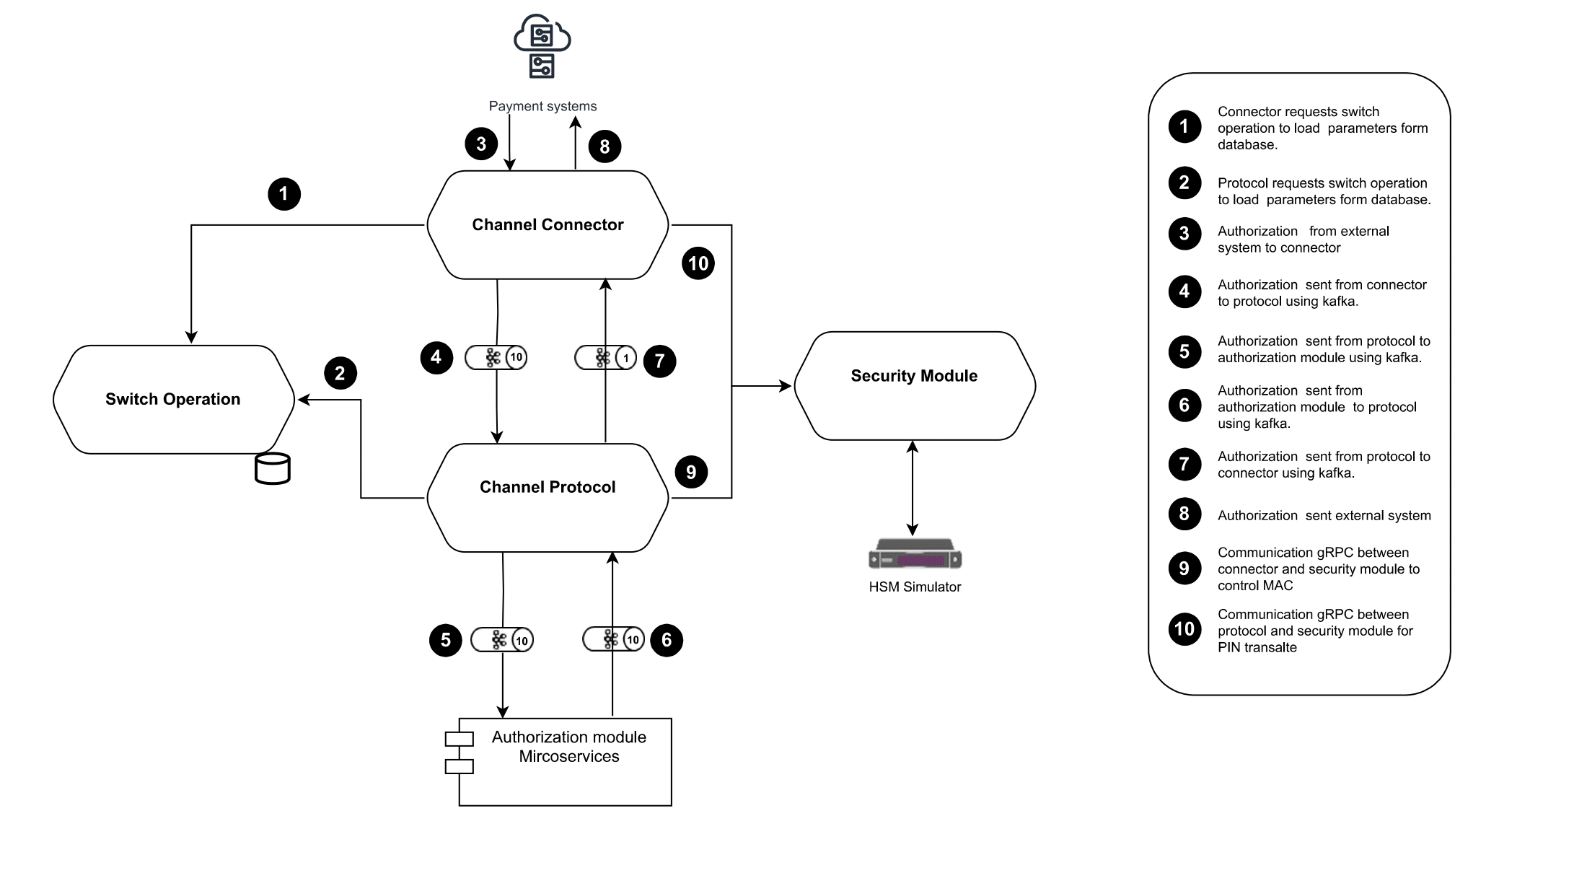
\includegraphics[width=7.19457in,height=3.95867in]{media/image50.png}
\caption{Microservices communication schema}
\label{fig:MCS}
\end{figure}

\begin{quote}
This diagram presents the general architecture of the authorization flow
within the Switch PowerCARD system. When an authorization request is
initiated (for example, from the Mastercard network), it is first
received by the Channel Connector, which interacts with the Switch
Operation module to load the necessary configuration parameters. The
authorization message is then published to a Kafka topic and consumed by
the Channel Protocol, which in turn forwards the request to the
authorization microservices. These microservices apply business logic
(fund validation, scoring, security rules, etc.) and return their
response to the Channel Protocol. The latter then constructs the
response message and publishes it again to Kafka so that the Channel
Connector can retrieve it and send it back to the external network. At
the same time, the Channel Protocol communicates with the security
module (HSM Simulator) via gRPC calls for sensitive processing: MAC
generation and validation, PIN data management. This decoupling by Kafka
ensures high availability and scalability of processing, while the use
of gRPC for the security layer guarantees efficient and secure
exchanges.
\end{quote}
\clearpage

\subsubsubsection{Channel connect diagram :}
\begin{quote}
\textbf{Abstract diagram :}
\end{quote}

\begin{quote}
The diagram above represents the abstract architecture of the Channel
Connector, a key component responsible for providing the interface
between the internal protocol and the Mastercard network. This component
also relies on a common SDK, providing the building blocks necessary to
implement a standardized and reusable network connector.

The processing is divided into Kafka pipelines and abstract
transformation functions:
\begin{itemize}
\item
  PwcChannelInboundConsumerSource receives inbound messages from the
  network (via a TCP/SSL interface) and injects them into the pipeline.
\item
  The Abstract inbound processor function applies protocol-specific
  processing (decoding, format verification, etc.).
\item
  Messages are then published to the protocol via PwcChannelProtocolSink
  on the pwc-net-in topic.
\end{itemize}
\end{quote}



\begin{quote}
\textbf{In reverse :}
\end{quote}

\begin{itemize}
\item
  Protocol output messages (pwc-net-out) are consumed by
  PwcChannelProtocolSource.
\item
  The Abstract protocol processor function prepares messages to be sent
  over the network.
\item
  PwcChannelOutboundSink provides transmission over the network
  interface (TCP/SSL).
\end{itemize}

\begin{quote}
\textbf{The connector also integrates :}
\end{quote}

\begin{itemize}
\item
  PwcChannelHeartbeatSink for real-time monitoring.
\item
  PwcChannelMetricSink for collecting technical metrics (published on
  the pwc-metric topic).
\item
  PwcChannelEventLogSink for event traceability, powering an OpenSearch
  (Elastic) engine.
\end{itemize}

\begin{quote}
This decoupled, Kafka-based architecture enables asynchronous, scalable,
and robust processing of Mastercard flows, while ensuring isolation
between protocol logic and network transport.
\begin{figure}[H]
\centering
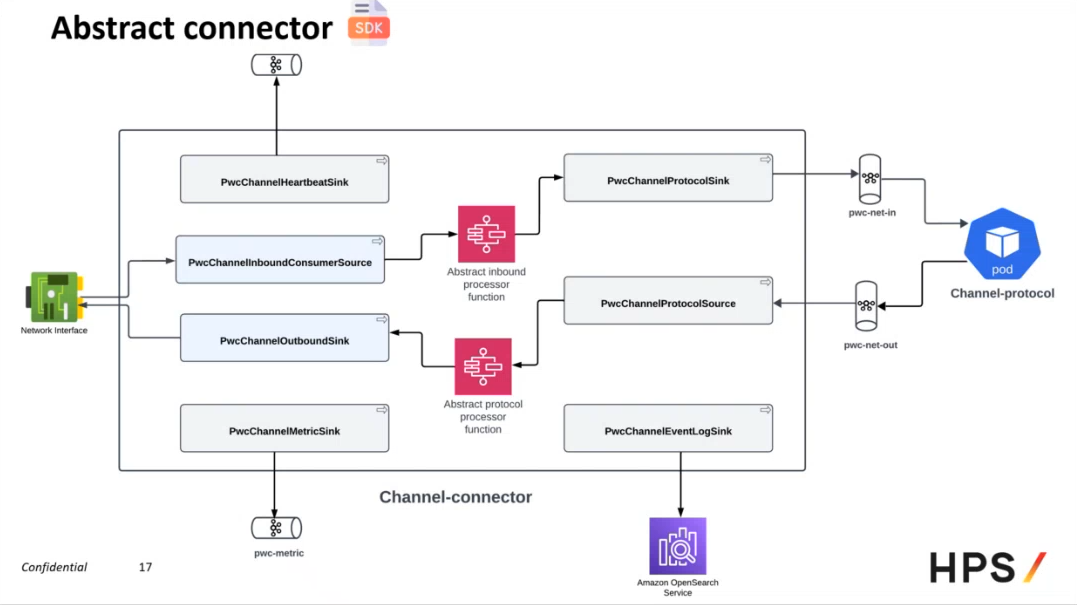
\includegraphics[width=6.03815in,height=3.38958in]{media/image51.png}
\caption{Abstract connector schema}
\label{fig:ACC}
\end{figure}

\end{quote}


\begin{quote}
\textbf{Incoming request:}
\end{quote}
\begin{quote}
This flow describes the processing of an incoming request (e.g., an
authorization request) within the Channel Connector microservice.

The authorization message is sent by the Mastercard network and captured
by the Channel Connector via a TCP connection. The message is then
temporarily stored in an internal memory queue.

A free thread, from the thread pool dedicated to processing
authorizations, takes charge of the message and performs format and
integrity checks.

If a MAC (Message Authentication Code) check is enabled, the message is
passed to the Security Module via gRPC call for verification.

After verification, the message is published to the Kafka topic
pwc-net-in, using a partition key derived from authorization elements,
to ensure correct ordering. This topic has multiple partitions, and
partition selection depends on the message key.

The message is then consumed by the Channel Protocol microservice for
further processing.
\end{quote}

\begin{figure}[H]
\centering
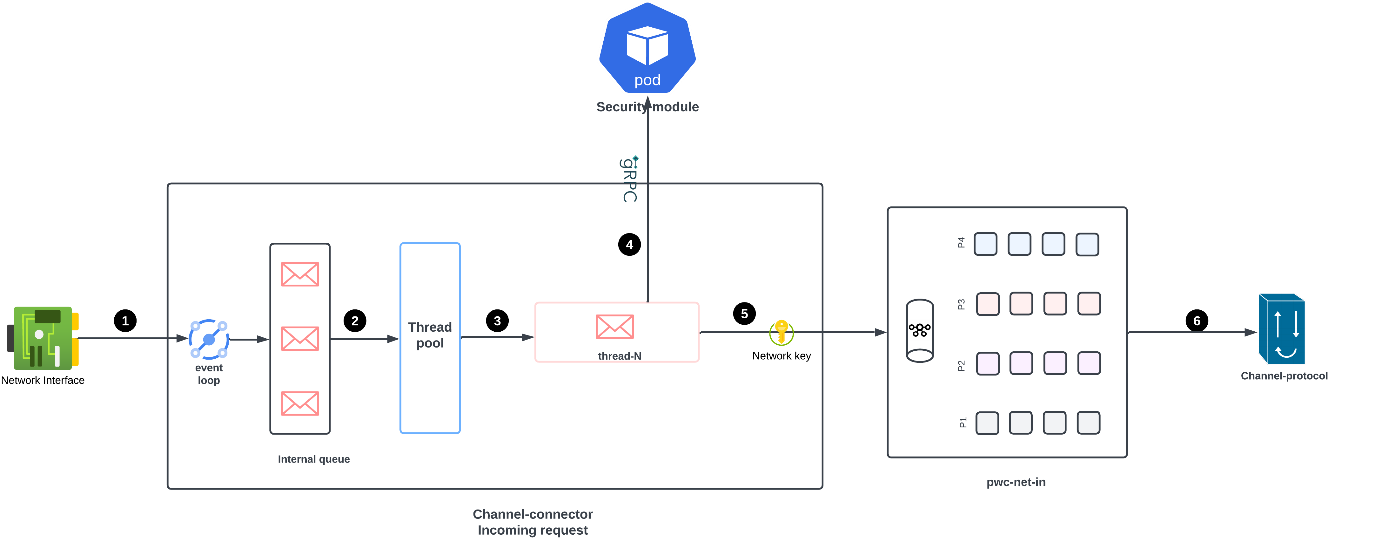
\includegraphics[width=6.22725in,height=2.48059in]{media/image52.png}
\caption{Incoming request explicative schema}
\label{fig:IRES}
\end{figure}

 

\begin{quote}
\textbf{Outgoing response:}
\end{quote}

\begin{quote}
This flow describes the processing of an outgoing response within the
Channel Connector (response to a previously issued request).

The authorization response message is sent by the Channel Protocol
microservice on the pwc-net-out (multi-partition) Kafka topic.

The Channel Connector consumes this message on its dedicated partition.
After consumption, the message is sent to the Mastercard network via the
TCP connection.

Finally, the connector publishes technical metrics on the observed
response time, by sending a message on the pwc-metric topic.
\end{quote}

\begin{figure}[H]
\centering
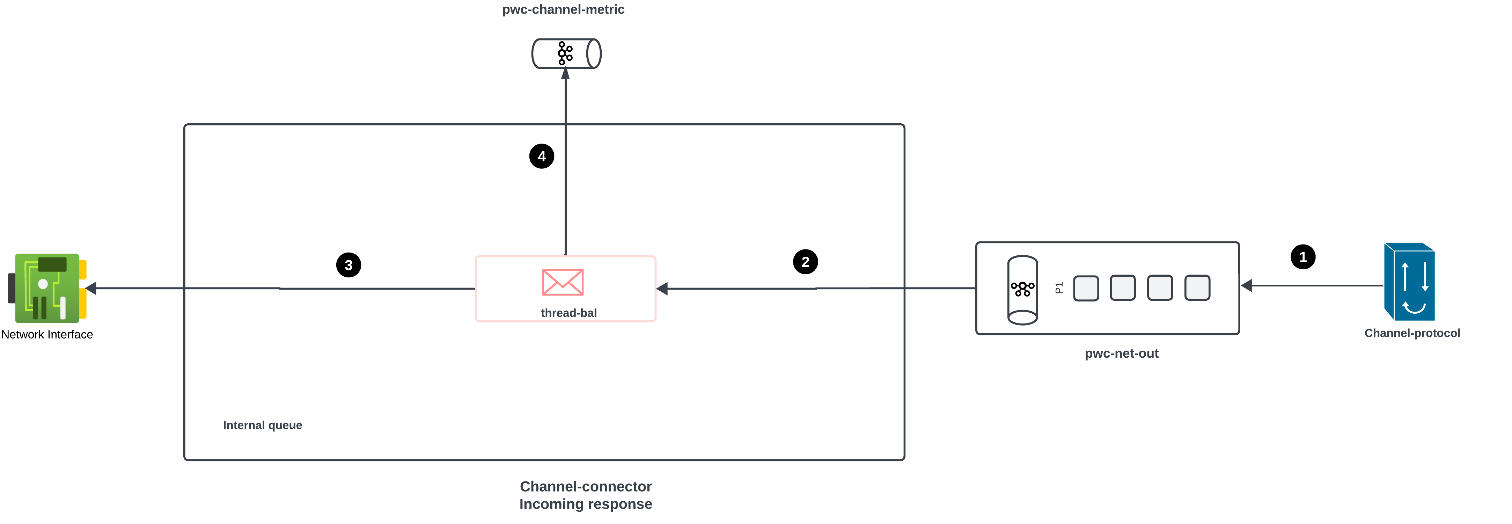
\includegraphics[width=6.84092in,height=2.37072in]{media/image53.png}
\caption{Outgoing response explicative schema}
\label{fig:ORES}
\end{figure}
 \clearpage

\begin{quote}
\textbf{Outgoing request:}
\end{quote}

\begin{quote}
This flow describes the processing of an outgoing request (request
generated on the Switch side to Mastercard).

The authorization message is published by the Channel Protocol on the
pwc-net-out (multi-partition) Kafka topic. The Channel Connector
consumes this message on a specific partition.

The authorization context is saved in a local RocksDB database (to allow
subsequent matches).

The message is then sent to the Mastercard network via the TCP
connection.
\end{quote}

\begin{figure}[H]
\centering
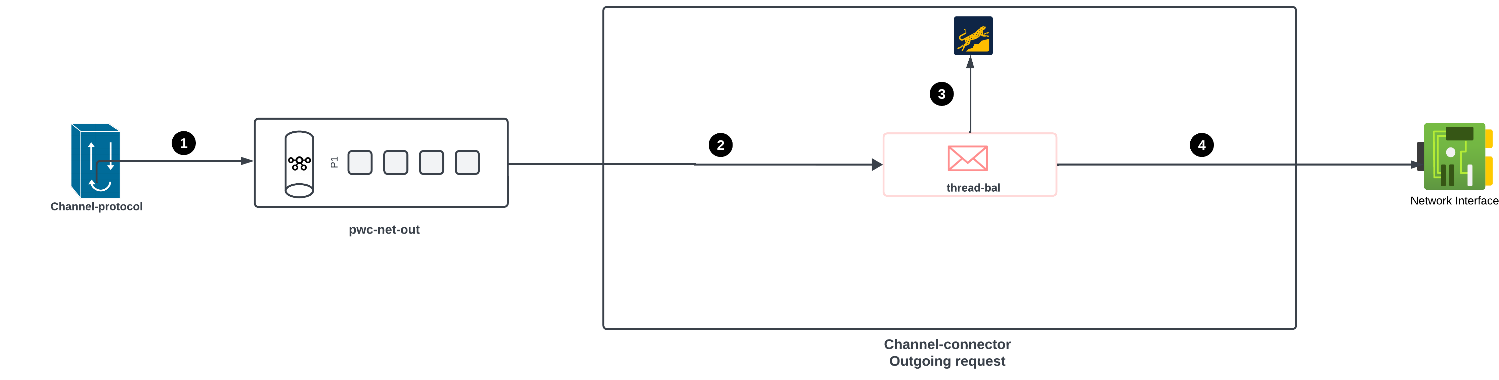
\includegraphics[width=6.78333in,height=1.72048in]{media/image54.png}
\caption{Outgoing request explicative schema}
\label{fig:ORES}
\end{figure}

\begin{quote}
\textbf{Incoming response :}
\end{quote}

\begin{quote}
This flow describes the processing of an incoming response (from
Mastercard) as part of an outgoing transaction (initiated by the
Switch).

The message is captured by the Channel Connector via TCP and then
temporarily stored in a memory queue.

A free thread from the processing pool takes over this message and
performs the format checks.

The Channel Connector then retrieves the corresponding authorization
context from RocksDB.

If MAC checking is enabled, the message is sent to the security module
via gRPC for verification.

Finally, the message is published to Kafka (pwc-net-in), with a
partition key consistent with the original context. The Channel Protocol
will consume this message to reconstruct the full authorization.
\end{quote}

\begin{figure}[H]
\centering
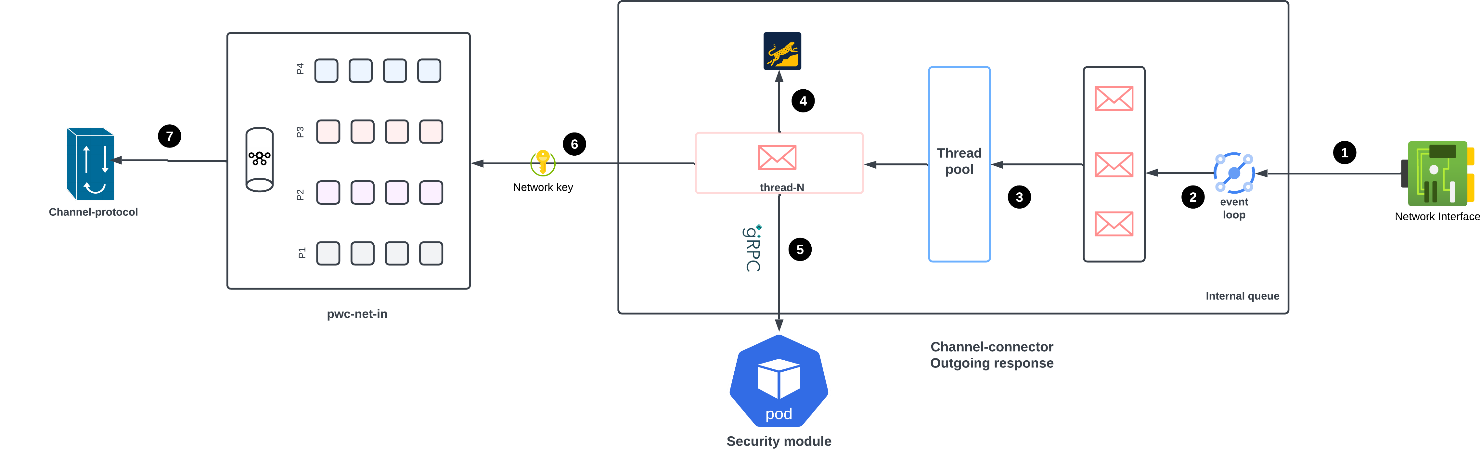
\includegraphics[width=6.70029in,height=2.03289in]{media/image55.png}
\caption{Incoming response explicative schema}
\label{fig:IRES}
\end{figure}



\subsubsubsection{Channel protocol diagram}
\begin{quote}
\textbf{Abstract diagram:}
\end{quote}

\begin{figure}[H]
\centering
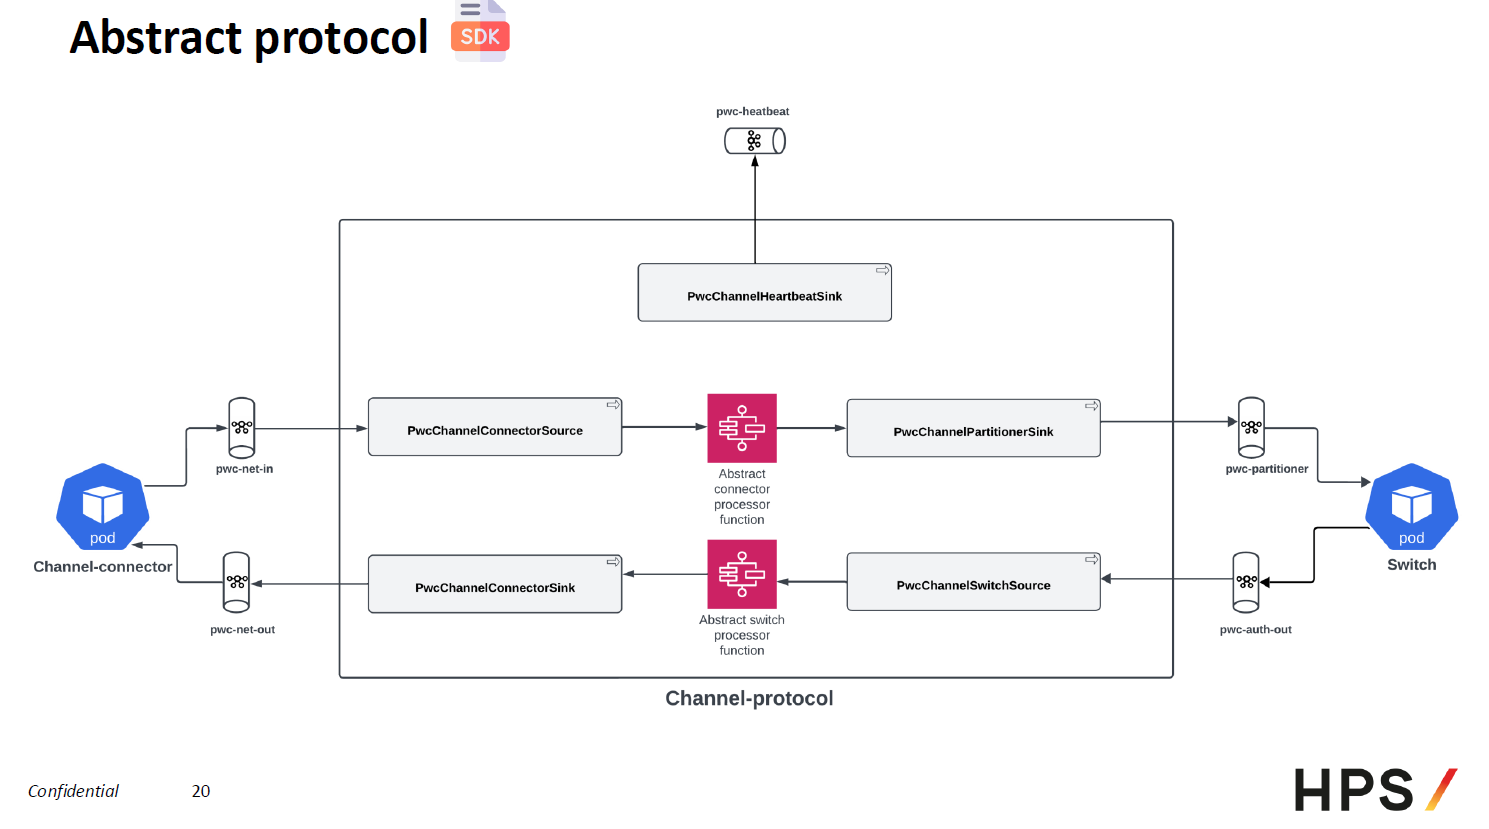
\includegraphics[width=6.58396in,height=3.38664in]{media/image56.png}
\caption{protocol abstract schema}
\label{fig:PBS}
\end{figure}

\begin{quote}
The abstract diagram above represents the logical architecture of the
Channel Protocol microservice, which is based on an SDK common to all
implemented protocols (CIS, ISO, SID, etc.). Its role is to ensure
generic interfacing between the Channel Connector (to the Mastercard
network) and the PowerCARD Switch (core business), using Kafka to
guarantee scalability and resilience.

The different components are specialized processors, each consuming and
publishing to dedicated Kafka topics:
\end{quote}

\begin{itemize}
\item
  PwcChannelConnectorSource consumes incoming network messages
  (pwc-net-in topic), performs protocol processing (e.g. CIS → ISO
  conversion), then publishes to PwcChannelPartitionerSink or
  PwcChannelSwitchSource depending on the business logic.
\item
  PwcChannelPartitionerSink publishes to the partitioned topic
  pwc-partitioner, which is consumed by the Switch for synchronous
  processing (e.g. authorization requests).
\item
  PwcChannelSwitchSource consumes business responses from the Switch
  (pwc-auth-out topic) and forwards them to the Connector via
  PwcChannelConnectorSink.
\item
  PwcChannelHeartbeatSink publishes heartbeat messages to monitor
  protocol health.
\end{itemize}

\begin{quote}
The SDK also provides abstract processing functions (Abstract connector
processor / Abstract switch processor), on which each protocol
implements its own business rules (e.g. CIS ⇄ ISO field mapping).

This modular approach makes it easy to implement new protocols, while
respecting a robust and validated common base.
\end{quote}

\begin{quote}
\textbf{Incoming request}
\end{quote}

\begin{quote}
The diagram below describes the processing flow of an incoming
authorization message within the Channel Protocol microservice.

The authorization message is sent to the Protocol microservice via the
pwc-net-in Kafka topic.

The Channel Protocol uses a Kafka consumer pool to read messages from
this topic.

A consumer thread retrieves the message and performs the protocol
conversion (CIS → ISO).

The original message is stored in a RocksDB database (allowing
correlation with the future response).

The message is then published to the Switch microservices via the
partitioned topic pwc-online-message-partitioner, the partition key
being based on business elements of the transaction (card number, STAN,
etc.).

Switch microservices then consume the message for business processing.
\end{quote}

\begin{figure}[H]
\centering
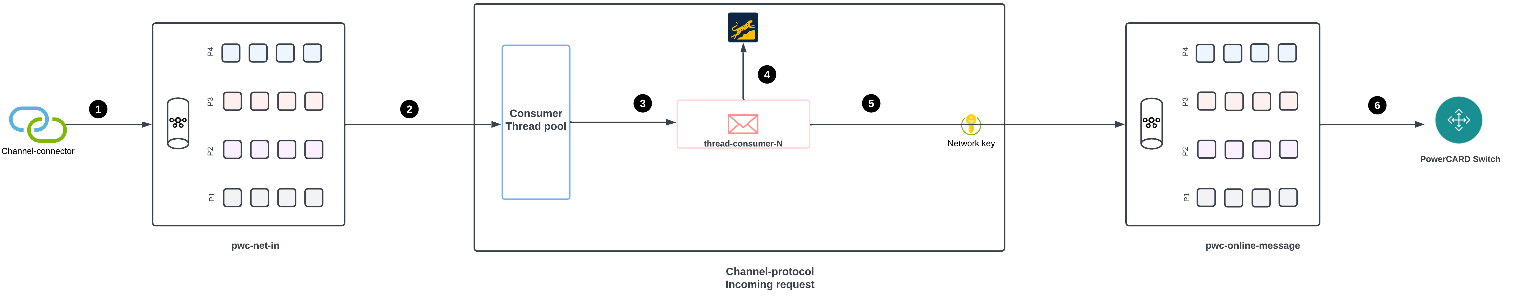
\includegraphics[width=6.95121in,height=1.35379in]{media/image57.png}
\caption{Incoming request schema}
\label{fig:IRS}
\end{figure}


\begin{quote}
\textbf{Incoming response}
\end{quote}


\begin{quote}
The following diagram describes the processing flow of an incoming
authorization response message within the Channel Protocol.

The response message is emitted by the Switch microservices on the Kafka
topic pwc-auth-out.

The Channel Protocol uses a pool of consumers to read messages on this
partitioned topic.

A consumer thread retrieves the message and performs the protocol
conversion.

The protocol retrieves the initial authorization request stored in
RocksDB to ensure consistency of the response message.

The message is then sent to the Connector via the pwc-net-in topic, to
be transmitted to the external network.
\end{quote}

\begin{figure}[H]
\centering
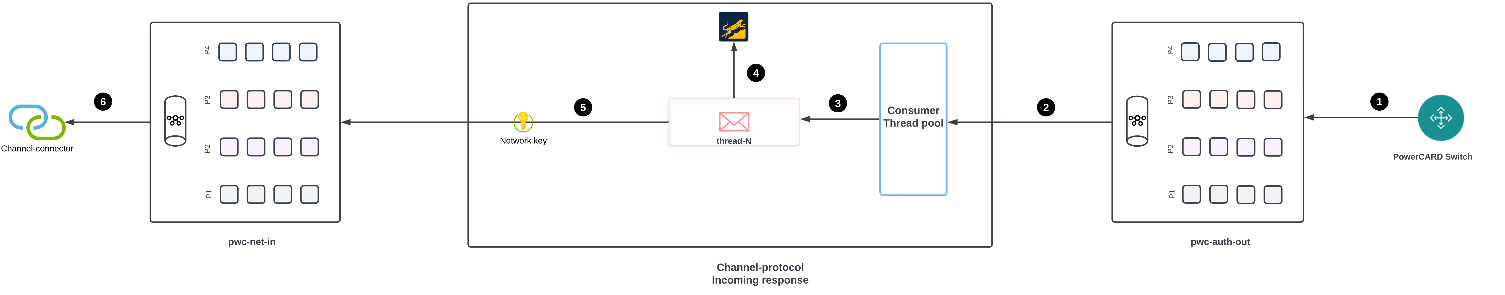
\includegraphics[width=6.82134in,height=1.33791in]{media/image58.png}
\caption{Incoming response schema}
\label{fig:}
\end{figure}


\begin{quote}
\textbf{Outgoing request}
\end{quote}

\begin{quote}
This diagram illustrates the processing flow of an outgoing request to
the external network.

The message is produced by the Switch microservices on the Kafka topic
pwc-auth-out.

The Channel Protocol consumes this message and performs the protocol
conversion.

If the request contains a PIN, the Channel Protocol calls the HSM module
(via gRPC) to perform the PIN translation.

The original message is stored in RocksDB.

The message is then published to the pwc-net-in topic to be transmitted
to the Connector, which relays it to the external network.
\end{quote}

\begin{figure}[H]
\centering
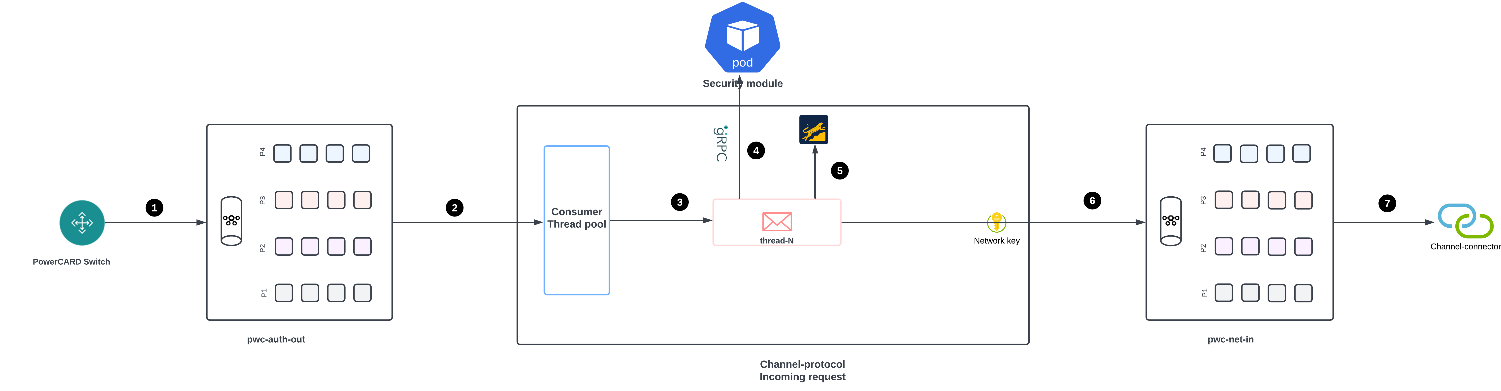
\includegraphics[width=6.79462in,height=1.77023in]{media/image59.png}
\caption{Outgoing request schema}
\label{fig:}
\end{figure}

\begin{quote}
\textbf{Outgoing response}
\end{quote}

\begin{quote}
Finally, the diagram below describes the processing of an outgoing
response.

The message is sent to the Channel Protocol via the Kafka topic
pwc-net-in.

The Channel Protocol consumes this message and performs the protocol
conversion.

It retrieves the original request from the RocksDB database, prepares
the response and publishes it to the Switch microservices via the
partitioned topic pwc-online-message-partitioner.

Switch microservices consume the message and continue business
processing.
\end{quote}

\begin{figure}[H]
\centering
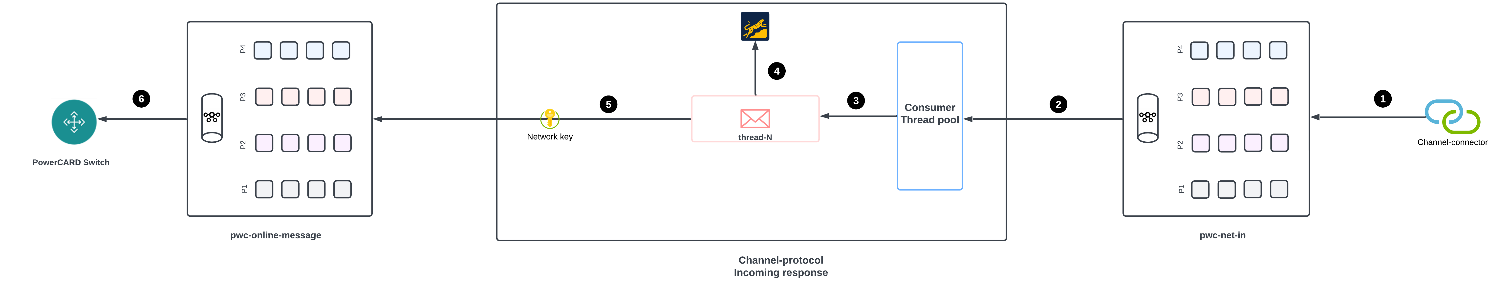
\includegraphics[width=6.72766in,height=1.29849in]{media/image60.png}
\caption{Outgoing response schema}
\label{fig:ORS}
\end{figure} 
\clearpage

\subsection{Conclusion :}

This chapter established the functional and conceptual foundations of
the Mastercard CIS protocol migration solution to the PowerCARD Switch
V4 architecture.

Through the analysis of requirements, the definition of use cases, and
the modeling of flows (sequence and activity diagrams), we clarified the
role of the key components Channel Protocol and Channel Connector as
well as their interactions with the various stakeholders in the payments
ecosystem: Mastercard network, the Switch, issuing and acquiring banks.

This work highlighted the inherent complexity of migrating a critical
payment protocol within a high-performance, real-time, and highly secure
transactional environment. The need to process heterogeneous flows
(acquiring/issuing, requests/responses, Authorization , Advice,
Reversals, File Updates) calls for a modular, scalable, and robust
architecture precisely what a microservices approach enables.

The different models produced (UML diagrams, message flows, context
management) also helped anticipate certain technical challenges related
to the migration, particularly the fine-grained handling of
authorization contexts, end-to-end message traceability, and smooth
integration with the legacy components of the Switch.

This analysis and design phase thus served as a key step to ensure a
structured, coherent, and standards-compliant implementation one that
meets the high demands of the banking and payments industry.



\clearpage

\section{Chapter 4: Implementing the Solution}


\subsection{Introduction
:}

This chapter presents the concrete technical implementation of the
microservices developed during this project: Channel Protocol and
Channel Connector.

The work also includes the development of the CIS SDK used by the
microservices, as well as the setting up of tests and validation
environments.

The project was carried out following the standards and practices of the
Online Product team, which provides a microservice skeleton generator
called Channel Initializer, included in the pwc-switch-v4-test-tools
project.



\begin{figure}[H]
\centering
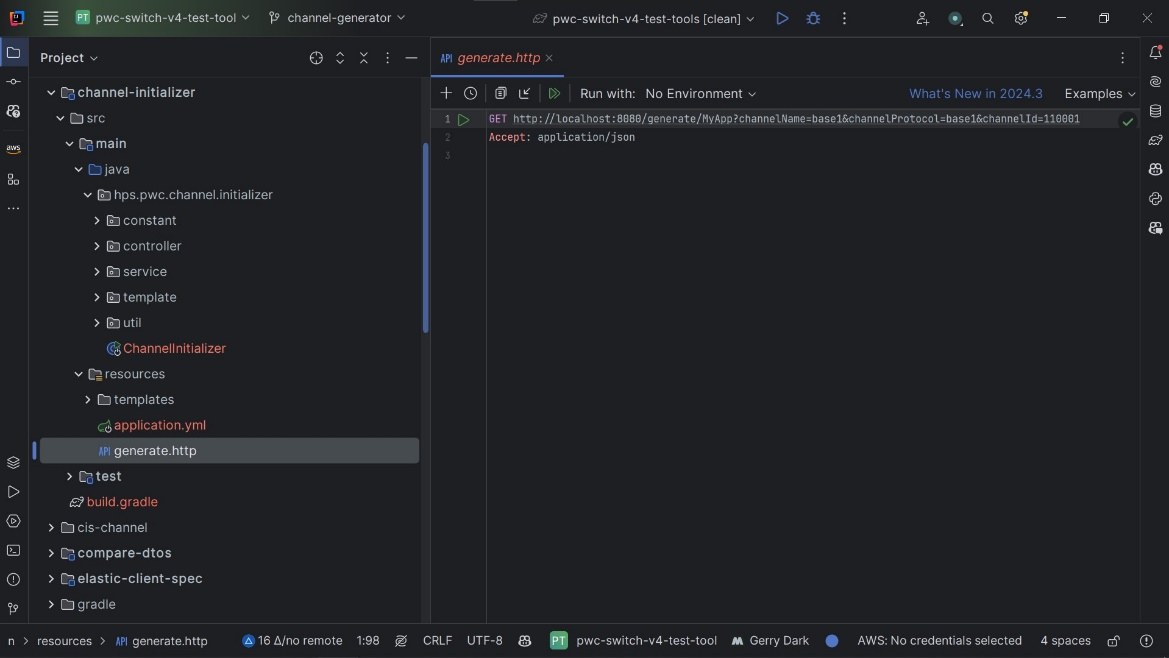
\includegraphics[width=5.29167in,height=2.97881in]{media/image61.jpeg}
\caption{Screenshot of the tool channel initializer}
\label{fig:TCI}
\end{figure} 


This generator provides the basic architecture common to all channels
developed around the Switch V4, and guarantees component consistency.
\begin{figure}[H]
\centering
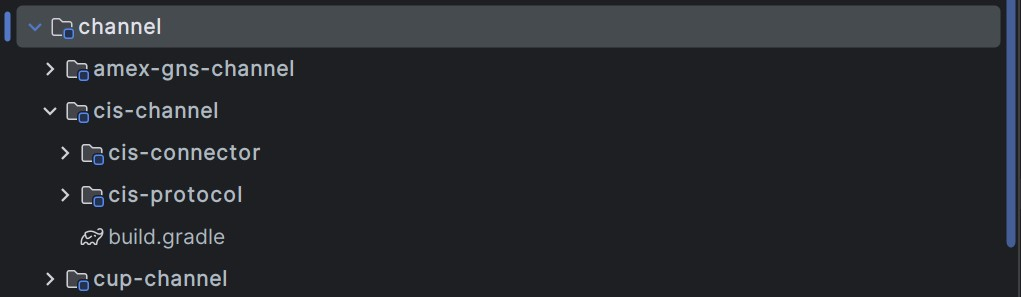
\includegraphics[width=\textwidth,height=\textheight,keepaspectratio]{media/image62.jpg}
\caption{Screenshot of the abstract skeleton of a channel cis}
\label{fig:ASC}
\end{figure} 




\subsection{1 - Connector microservice implementation:}

\begin{figure}[H]
\centering
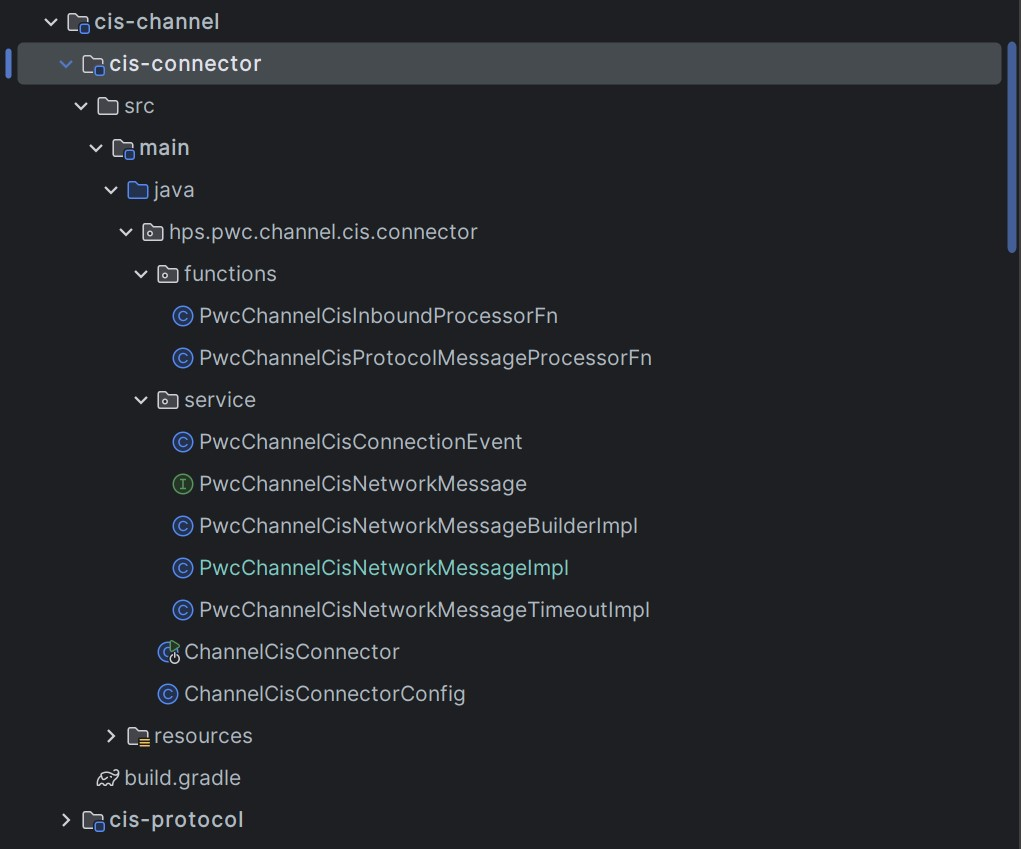
\includegraphics[width=\textwidth,height=\textheight,keepaspectratio]{media/image63.jpg}
\caption{Screenshot of the connector microservice structure}
\label{fig:CMS}
\end{figure} 

The Channel Connector microservice relies on several internal
dependencies: a channel core, an abstract SDK for the protocol, a
library for managing TCP/IP communications, advanced logging tools, and
an SDK for managing Kafka streams.

The development work consisted of migrating and reimplementing in Java
all the network logic from the legacy C code.

This includes in particular:

\begin{itemize}
\item
  Management of Network Management type messages (0800 and 0820 session
  management messages), allowing connection/disconnection operations and
  network status verification to be processed.
\item
  Processing of cryptographic key exchanges with the network, necessary
  for the proper establishment of secure sessions.
\item
  The implementation of a robust initial connection mechanism,
  incorporating several automatic attempts in the event of failure, in
  order to ensure maximum availability of services.
\item
  Implementation of network message sending functions (connect,
  disconnect, echo test), adapting specific cases from the C standard to
  consistent processing in Java.
\end{itemize}

Thanks to this work, all processing related to network management was
able to be migrated and stabilized in the Connector microservice,
respecting Java best practices and the overall architecture of the
project.


\subsection{2 - Implementation of the Protocol microservice}

\begin{figure}[H]
\centering
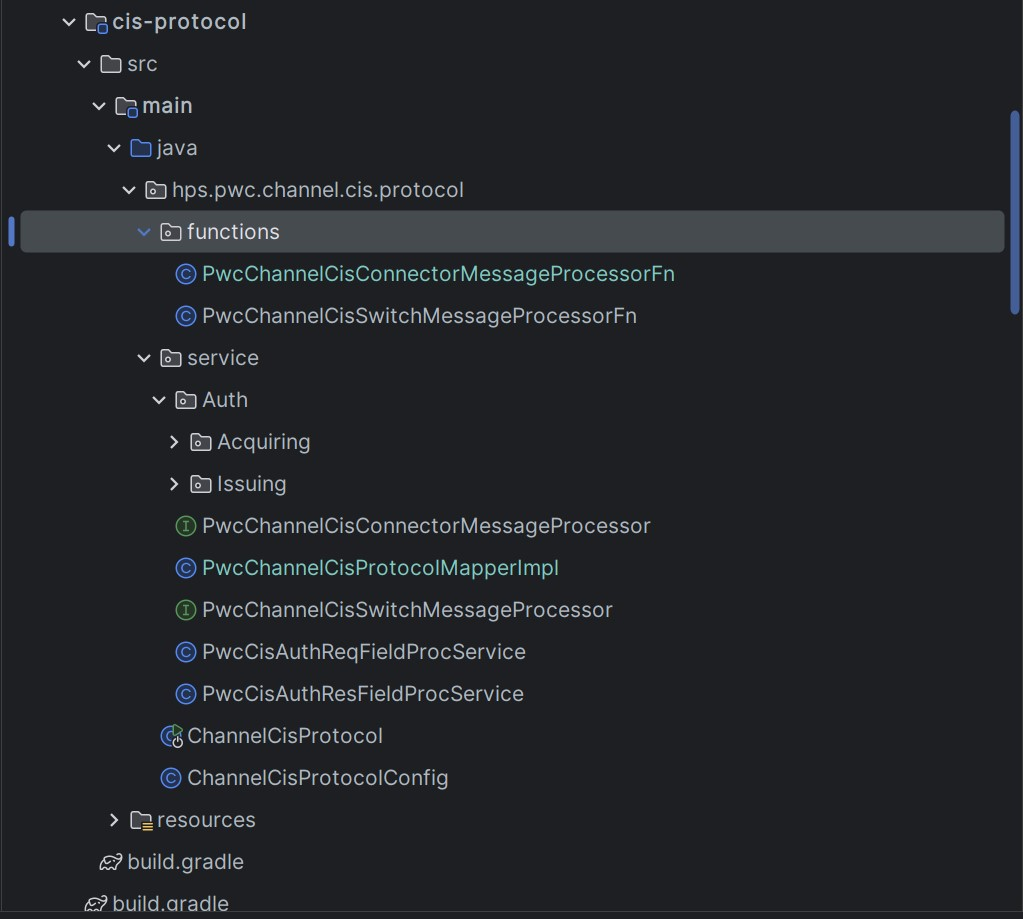
\includegraphics[width=\textwidth,height=\textheight,keepaspectratio]{media/image64.jpg}
\caption{Screenshot of the protocol microservice structure}
\label{fig:PMS}
\end{figure} 


The Channel Protocol microservice is built on an abstract common SDK
that provides the technical foundations needed to implement the
protocol.

The adopted software architecture is based on a modular model allowing
the processing flows between acquiring and issuing transactions to be
clearly separated.

For each type of message whether it\textquotesingle s an authorization
request, a reversal, an advice, or a file update dedicated components
are responsible for orchestrating the processing.

These components rely on mappers and utilities to perform message
conversion between ISO 8583 and CIS formats, in both directions.

The core of the business logic comes from the migration of several
source files from legacy C code (management of advices, file updates,
network communication, reversals and authorizations). This logic was
translated into Java while respecting the framework constraints and
integrating modern best development practices.

The CIS SDK, developed in parallel, provides all the constants,
enumerations, and utilities necessary for the consistency and
reliability of the processing carried out in the Protocol.


\subsection{3 - CIS SDK Development}
\begin{figure}[H]
\centering
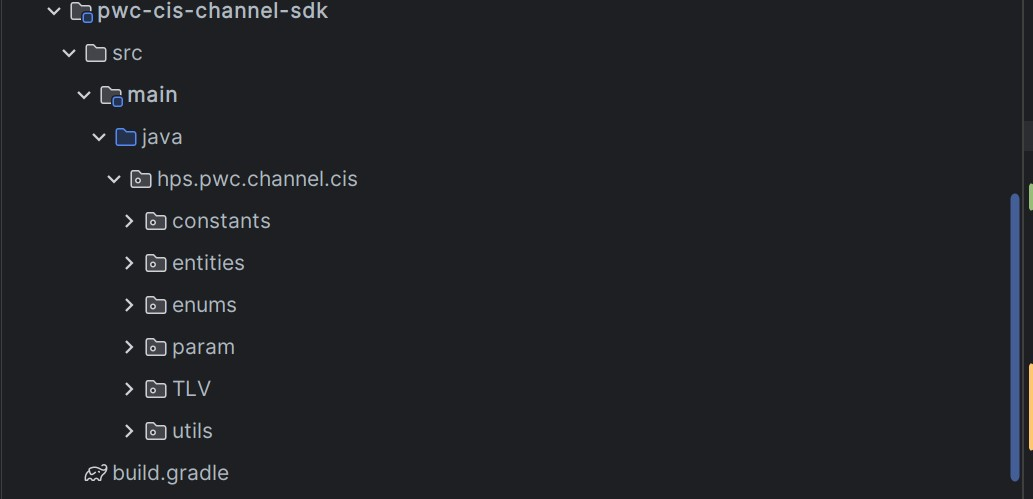
\includegraphics[width=\textwidth,height=\textheight,keepaspectratio]{media/image65.jpg}
\caption{Screenshot of the CIS SDK structure}
\label{fig:CSS}
\end{figure} 


The SDK allows you to factor out all the constants, enumerations,
utilities, and parameters needed by the Protocol and Connector
microservices.

The SDK contains the following:

\begin{itemize}
\item
  All CIS enumerations
\item
  Functions for tlv processing not handled by the abstract SDK or other
  SDK
\item
  CisFieldUtils: file that manages all repetitive processing in the
  project fields
\item
  PwcCisMessageFormatBuilder: this file creates a map for all the fields
  to build the incoming and outgoing Cis message, this file processes it
  by obligatoi
\item
  Format/Size Constants
\item
  \begin{quote}
  Parameterized management entities (loading tables)
  \end{quote}
\item
  \begin{quote}
  Functional utilities:
  \end{quote}
\item
  \begin{quote}
  buildCisMessageHeader
  \end{quote}
\item
  \begin{quote}
  getMcEpiArea
  \end{quote}
\end{itemize}

\begin{itemize}
\item
  \begin{quote}
  getCountryAlphaCode
  \end{quote}
\item
  \begin{quote}
  isoToCisAdditionalAmounts
  \end{quote}
\item
  \begin{quote}
  MciToIsoMdesMemberDefData
  \end{quote}
\end{itemize}

\begin{quote}
This SDK ensures consistency between treatments and simplifies future
evolution.
\end{quote}


\subsection{4 - Integration tests of migrated
microservices:}

\begin{quote}
To prepare the integration test environment, we used Docker Desktop to
orchestrate and monitor the various necessary containers, such as Kafka,
Zookeeper, and infrastructure services. the Docker Desktop interface
allows you to view the status of the containers, check their resource
consumption, and easily access exposed ports, facilitating rapid
deployment of the environment.
\end{quote}

\begin{figure}[H]
\centering
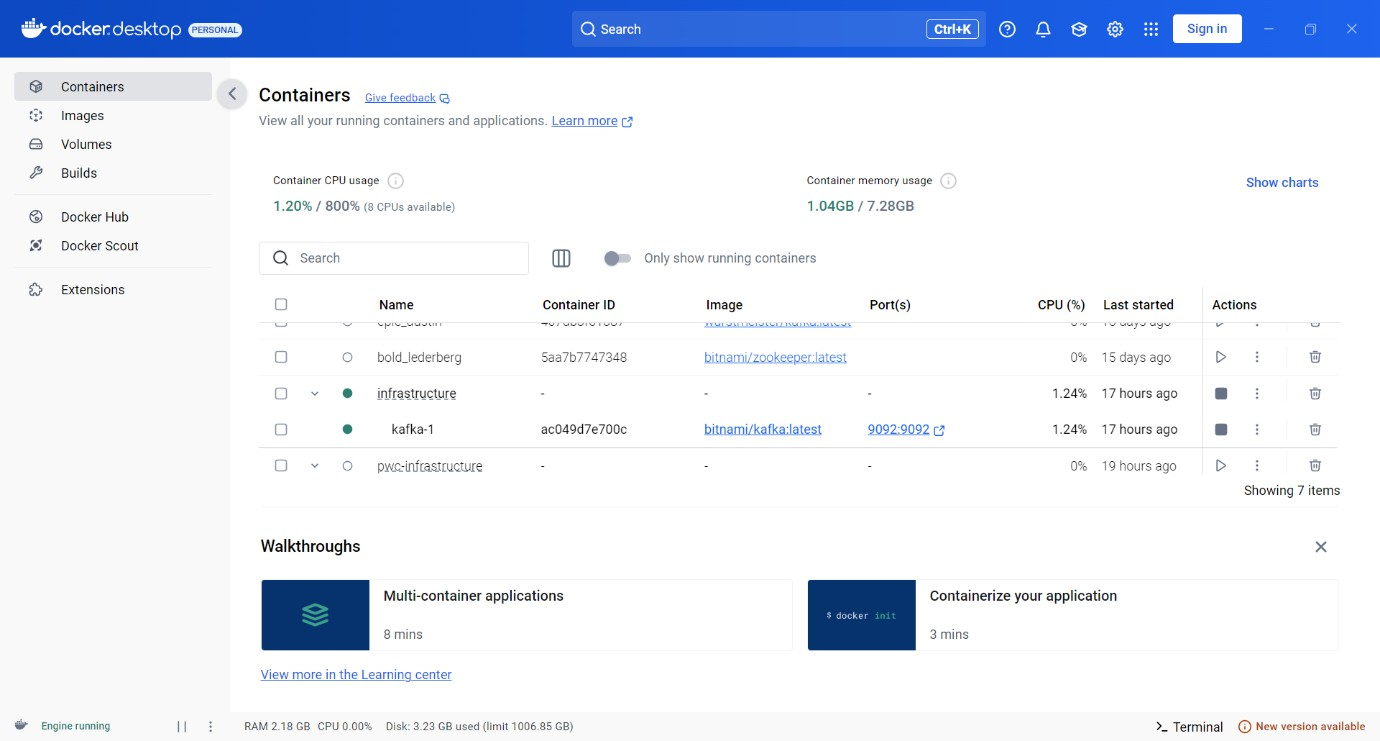
\includegraphics[width=\textwidth,height=\textheight,keepaspectratio]{media/image66.jpeg}
\caption{Screenshot of the Docker containers}
\label{fig:DC}
\end{figure} 

\begin{quote}
For the OpenLens setup, we added the clusters as shown in the following
screenshot . Once connected to the cluster via double-click, we selected
the Services tab under Config, then searched for and clicked on the
postgresql service The exposed port (5432) was then forwarded to the
application.yaml file to ensure connectivity with the database.

\begin{figure}[H]
\centering
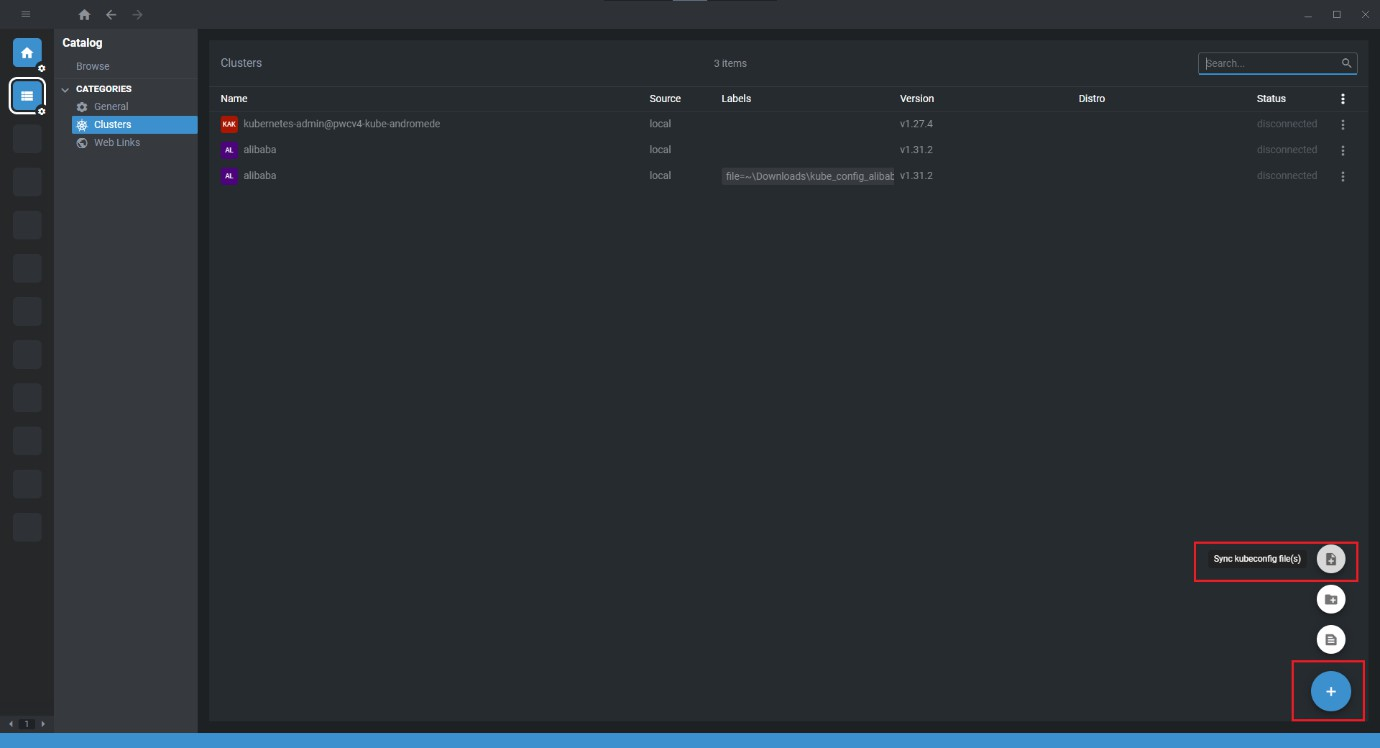
\includegraphics[width=\textwidth,height=\textheight,keepaspectratio]{media/image67.jpeg}
\caption{Screenshot of Openlens : clusters}
\label{fig:OC}
\end{figure} 

\end{quote}
\begin{quote}

\begin{figure}[H]
\centering
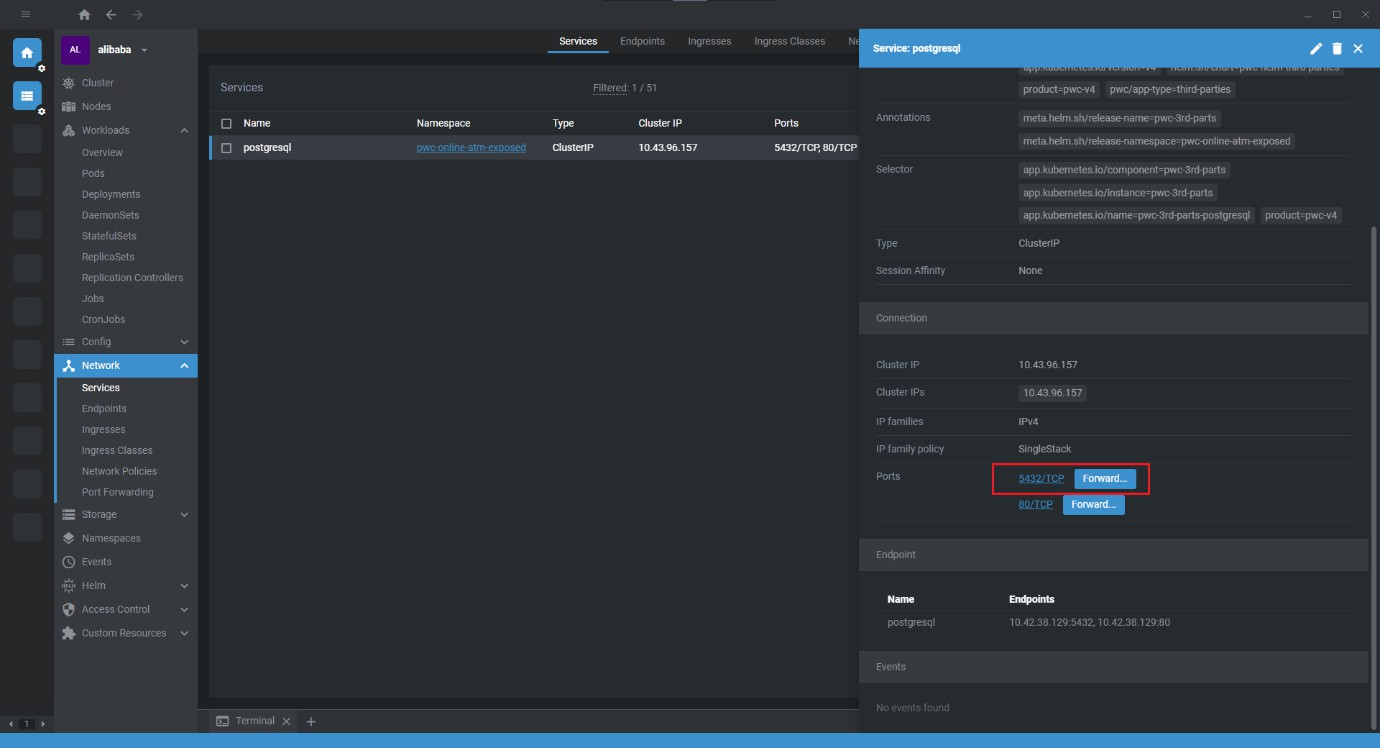
\includegraphics[width=\textwidth,height=\textheight,keepaspectratio]{media/image68.jpeg}
\caption{Screenshot of Openlens : forwarding the DB postgresql}
\label{fig:OFDP}
\end{figure} 

\end{quote}
\clearpage

We then launched the KafkaComposeUp task under Docker tasks :

\begin{figure}[H]
\centering
\includegraphics[width=\textwidth,height=\textheight,keepaspectratio]{media/image69.jpeg}
\caption{Screenshot of xml config to read the forwarded config}
\label{fig:XCRFC}
\end{figure} 

Once the service is started, the Kafka environment is
\begin{figure}[H]
\centering
\includegraphics[width=\textwidth,height=\textheight,keepaspectratio]{media/image70.jpeg}
\caption{Screenshot of out of kafka compose up}
\label{fig:XCRFC}
\end{figure} 



\begin{figure}[H]
\centering
\includegraphics[width=\textwidth,height=\textheight,keepaspectratio]{media/image71.jpeg}
\caption{Screenshot of images up in docker}
\label{fig:OFDP}
\end{figure} 


\begin{quote}
After setting up Kafka, we started the CIS Channel connector :
\end{quote}

\begin{figure}[H]
\centering
\includegraphics[width=\textwidth,height=\textheight,keepaspectratio]{media/image72.jpeg}
\caption{Screenshot of how to lunch the connector}
\label{fig:OFDP}
\end{figure} 


\begin{quote}
Once fired, the onOpenConnection event initiates sending a signon
message to the PSTT simulator, which in turn responds.
\end{quote}

\begin{figure}[H]
\centering
\includegraphics[width=\textwidth,height=\textheight,keepaspectratio]{media/image73.jpeg}
\caption{Screenshot of the results Sending sign on message}
\label{fig:OFDP}
\end{figure} 


\begin{figure}[H]
\centering
\includegraphics[width=\textwidth,height=\textheight,keepaspectratio]{media/image74.jpeg}
\caption{Screenshot of the
results PSTT response}
\label{fig:RPR}
\end{figure} 

We then started the protocol microservice and the switch simulator:

\begin{figure}[H]
\centering
\includegraphics[width=\textwidth,height=\textheight,keepaspectratio]{media/image75.jpeg}
\caption{Screenshot of steps to
lunch protocol}
\label{fig:SLP}
\end{figure} 

At this point, it is possible to send an authorization message from the
PSTT simulator and observe the traces generated at each step:

\begin{figure}[H]
\centering
\includegraphics[width=\textwidth,height=\textheight,keepaspectratio]{media/image76.jpeg}
\caption{Screenshot of results
when Sending the message from the PSTT}
\label{fig:SMP}
\end{figure} 

\begin{figure}[H]
\centering
\includegraphics[width=\textwidth,height=\textheight,keepaspectratio]{media/image77.jpeg}
\caption{Screenshot of results
Receiving the incoming message in the connector}
\label{fig:RIMC}
\end{figure} 


\begin{figure}[H]
\centering
\includegraphics[width=\textwidth,height=\textheight,keepaspectratio]{media/image78.jpeg}
\caption{Screenshot of results
Sending the connector response to the PSTT}
\label{fig:SCRP}
\end{figure} 




\begin{figure}[H]
\centering
\includegraphics[width=\textwidth,height=\textheight,keepaspectratio]{media/image79.jpeg}
\caption{Screenshot of results
receiving the message in the protocol}
\label{fig:RRMP}
\end{figure} 

\begin{figure}[H]
\centering
\includegraphics[width=\textwidth,height=\textheight,keepaspectratio]{media/image80.jpeg}
\caption{Screenshot of results Transformation of the message to the ISO Switch protocol}
\label{fig:RRMP}
\end{figure} 



\begin{figure}[H]
\centering
\includegraphics[width=\textwidth,height=\textheight,keepaspectratio]{media/image81.jpeg}
\caption{Screenshot of results
Receiving the response from the switch simulator}
\label{fig:RRSS}
\end{figure} 


\begin{figure}[H]
\centering
\includegraphics[width=\textwidth,height=\textheight,keepaspectratio]{media/image82.jpeg}
\caption{Screenshot of results
Transformation of the response to the external protocol}
\label{fig:RTREP}
\end{figure} 

\begin{quote}
This sequence illustrates the complete journey of an authorization
message, from initiation to response, passing through all key components
of the migrated architecture
\end{quote}


\subsection{Conclusion :}

\begin{quote}
The implementation work carried out during this project made it possible
to thoroughly modernize the management of the CIS protocol by migrating
most of the logic inherited from the C code to a microservices-oriented
Java architecture. Thanks to this approach, the processing is now more
modular, maintainable, and aligned with the technical standards of the
Switch V4 ecosystem.

The microservices developed (Channel Protocol and Channel Connector), as
well as the associated CIS SDK, now offer a robust and consistent basis
for processing acquiring and issuing flows, ensuring compatibility with
Mastercard specifications and production requirements.

The project allowed for the full use of modern technologies such as
Kafka for asynchronous exchanges, gRPC for secure communication with the
HSM module, and RocksDB for managing transactional contexts.

Among the most complex technical aspects, we can cite the fine migration
of the Reversals logic, the management of Advice (specific business
cases) and the porting of network management to TCP/IP.

This work also enabled significant skill development on the following
themes:
\end{quote}

\begin{itemize}
\item
  \begin{quote}
  Distributed microservices architecture
  \end{quote}
\item
  \begin{quote}
  Asynchronous processing and Kafka stream management
  \end{quote}
\item
  \begin{quote}
  Payment security (MAC, PIN translation via HSM)
  \end{quote}
\item
  \begin{quote}
  Software industrialization and compliance with good development
  practices
  \end{quote}
\end{itemize}

\begin{quote}
This technical foundation paves the way for the evolution and future
extension of the capabilities of the CIS protocol within the Switch V4.
\end{quote}
\clearpage


\section{Chapter 5: Architecture and technologies
}


\subsection{Introduction :}

\begin{quote}
The objective of this chapter is to present the general software
architecture of the developed solution, as well as the main technologies
and tools used within the framework of the project.

The chosen architecture is based on a microservices approach, allowing
for better separation of responsibilities, fine scalability of
components, and easier maintenance. As the CIS protocol plays a critical
role in real-time transaction processing, it was essential to guarantee
optimal performance and strong system resilience.

The technological choices were guided by the standards in force in the
Online Product team, while taking into account the specificities of the
CIS protocol and the requirements of Switch V4.

In this chapter, we will detail:
\end{quote}

\begin{itemize}
\item
  \begin{quote}
  The overall architecture of the system
  \end{quote}
\item
  \begin{quote}
  The main technical building blocks used
  \end{quote}
\item
  \begin{quote}
  Development and industrialization tools
  \end{quote}
\item
  \begin{quote}
  The deployment and testing environment
  \end{quote}
\end{itemize}


\subsection{1 - Functional architecture}

\begin{quote}
The Channel V4 architecture is based on several specialized layers:
\end{quote}

\begin{itemize}
\item
  \begin{quote}
  \textbf{Connector}: manages the network communication layer in TCP/IP,
  ensuring the reading/writing of messages to/from external networks
  (Mastercard, Visa, etc.).
  \end{quote}
\item
  \begin{quote}
  \textbf{Protocol}: manages the conversion of messages between the
  external format (CIS, ISO 8583, etc.) and the internal format of the
  Switch V4. It also performs message conformity checks.
  \end{quote}
\item
  \begin{quote}
  \textbf{Gateway}: allows handling of HTTP communications for other
  channel types (not used here for CIS).
  \end{quote}
\item
  \begin{quote}
  \textbf{Channel}: global orchestration layer that assembles the
  Protocol and Connector components.
  \end{quote}
\end{itemize}

\begin{quote}
This division ensures a clear separation of responsibilities and
facilitates the maintenance and evolution of components.
\end{quote}


\subsection{2 - Application architecture: from C
monolith to Java microservices
:}

\begin{quote}
The CIS (Channel Interface System) protocol implementation has
transitioned from a tightly coupled C-based monolith to a modular
microservice architecture, meticulously designed to adhere to core
software engineering principles.

\textbf{Monolithic Legacy:}

The original CIS implementation suffered from the classic limitations of
a monolithic design:
\end{quote}

\begin{itemize}
\item
  \textbf{Tight Coupling:}~The C codebase exhibited high coupling
  between core functionalities, hindering maintainability and evolution.
  The specific areas of coupling were:

  \begin{itemize}
  \item
    OSI communication with external components
  \item
    \textbf{Network Communication Layer:}~Handling the CIS
    protocol\textquotesingle s network interactions was intertwined with
    other logic.
  \item
    \textbf{Business Logic (ISO ↔ CIS Mapping):}~The translation between
    ISO 8583 (or another financial standard) and the specific CIS
    protocol was not cleanly separated.
  \item
    \textbf{Transaction Management:}~Functions like acquiring, issuing,
    and reversal processing were tightly integrated.
  \end{itemize}
\item
  \textbf{Deployment Challenges:}~Any update, regardless of scope,
  required a full recompilation and redeployment of the entire system.
\item
  \textbf{Limited Scalability:}~It was impossible to scale specific
  components independently to address performance bottlenecks.
\item
  \textbf{Reduced Resilience:}~A single failure point could bring down
  the entire CIS processing chain.
\end{itemize}

\begin{quote}
\textbf{Microservice Transformation (Design-Centric):}

To overcome these limitations, we migrated to a microservices
architecture, emphasizing a clean separation of concerns and adherence
to SOLID principles. This design emphasizes:
\end{quote}

\begin{itemize}
\item
  \textbf{Decoupling and Modularity:}~The CIS channel is now decomposed
  into smaller, independent services such as:

  \begin{itemize}
  \item
    \textbf{Connector Service:}~Handles network connectivity,
    protocol-specific interactions, and initial message processing.
    Think of this as the "edge" of the CIS channel, responsible for
    interfacing with external CIS systems.
  \item
    \textbf{Protocol Service:}~Responsible for CIS-specific data
    validation, transformation, and mapping to internal domain objects.
    Implements the specific ISO ↔ CIS mapping.
  \item
    \textbf{Services per Transaction (Acquiring, Issuing):}~Further
    decomposition could lead to separate microservices dedicated to
    specific transaction types, allowing for granular scaling and
    specialization.
  \end{itemize}
\item
  \textbf{The design respects the SOLID}~This pattern ensures that each
  service is maintainable and testable on its own

  \begin{itemize}
  \item
    \textbf{S (Single Responsibility):}~Each service follows Single
    Responsibility so it doesn\textquotesingle t have different reason
    to change.
  \item
    \textbf{O (Open Close):}~New functionality can be added (extended)
    without altering the code already implemented in those modules. For
    example the addition of a new Acquirer will not alter the service.
  \item
    \textbf{L (Liskov Substitution):}~It is respected so an object can
    be passed as super class and still behave as expected.
  \item
    \textbf{I (Segregation):}~No one class implements all methods they
    should implement some of them (and only the needed)
  \item
    \textbf{D (Inversion of Dependency):}~Modules don\textquotesingle t
    depend on concrete classes, but abstraction.
  \end{itemize}
\item
  \textbf{Design Pattern Utilization:}

  \begin{itemize}
  \item
    \textbf{Repository Pattern:}~Abstraction of data access, promoting
    testability and decoupling from specific data storage technologies.
  \item
    \textbf{Factory Pattern:}~Dynamic construction of routing paths
  \item
    \textbf{Adapter Pattern:}~Abstracts complexities from external
    third-party libraries
  \item
    \textbf{Strategy Pattern:}~Utilized to add new services and
    processes without altering the old ones.
  \end{itemize}
\item
  \textbf{SDK-Driven Development:}~A dedicated SDK encapsulates
  CIS-specific data structures, enumerations, and utility functions to
  provide a consistent and reusable interface for developers working
  with the CIS channel. This reduces code duplication and promotes
  adherence to the CIS protocol standards.
\item
  \textbf{Benefits Realized:}

  \begin{itemize}
  \item
    \textbf{Improved Modularity:}~The clear separation between the
    Connector and Protocol services significantly improves code
    organization and maintainability.
  \item
    \textbf{Independent Scalability:}~We can now scale the Connector
    service to handle increased network traffic or scale the Protocol
    service if complex mapping logic becomes a bottleneck.
  \item
    \textbf{Enhanced Resilience:}~Failures in the Connector service
    (e.g., network issues) do not necessarily impact the Protocol
    service, and vice versa. This is a consequence of decoupling.
  \item
    \textbf{Faster Deployment Cycles:}~Teams can iterate and deploy
    updates to individual microservices without affecting other parts of
    the system.
  \item
    \textbf{Increased Interoperability:}~Enables seamless integration
    with other services within the ecosystem, facilitating new
    functionalities like real-time fraud monitoring.
  \end{itemize}
\end{itemize}

\subsection{3 - Main technologies
used :}
\begin{quote}
The development is based on a modern technological foundation consistent
with industry standards:
\end{quote}

\begin{figure}[H]
\centering
\includegraphics[width=2in]{media/image83.png}
\caption{Spring boot logo}
\label{fig:SBL}
\end{figure} 


\begin{quote}
In the backend part of the application, the company required us to use
the Spring Boot Java Framework. From my research I have done I found
that Spring Boot greatly facilitates application development by
providing default configurations and automating many common tasks.

This allowed us to focus on business logic rather than technical
configuration.
\end{quote}

\begin{itemize}
\item
  Spring Boot is well-suited to microservice architecture. My teammates
  and I were each tasked with developing a specific microservice.
\item
  Spring Core: The foundation of the Spring ecosystem, it manages
  dependency injection, includes Spring MVC for the web and modules for
  database access.
\item
  Spring Data: Allows you to easily communicate with different types of
  databases using interfaces and naming conventions.
\item
  Spring Security: Essential module for authentication, authorization,
  and API security, although complex to master.
\item
  Spring Cloud: Key tool for administration and tolerance
\item
  to failures in microservices architectures.
\item
  Spring Boot: Simplifies autoconfiguration, dependency management,
  monitoring, and deployment of Spring applications.
\end{itemize}

\begin{quote}
The team systematically used Spring Initializr (start.spring.io) to
quickly generate suitable Spring Boot projects with the necessary
dependencies, which standardized the configuration and reduced the risk
of errors.
\end{quote}

\begin{figure}[H]
\centering
\includegraphics[width=2in]{media/image84.png}
\caption{Spring integration
logo}
\label{fig:SIL}
\end{figure} 


\begin{quote}
Spring Integration makes it easy to implement complex message flows
between components:
\end{quote}

\begin{itemize}
\item It provides communication channels (MessageChannel),
\item adapters (KafkaAdapter),
\item routers and filters.
\end{itemize}

This allows for the construction of robust, easily testable and reusable
flows.

Channels used:

\begin{itemize}
\item QueueChannel
\item PriorityChannel
\item DirectChannel
\item ExecutorChannel
\end{itemize}
\clearpage

\begin{figure}[H]
\centering
\includegraphics[width=1.5in]{media/image85.png}
\caption{kafka logo}
\label{fig:SIL}
\end{figure} 

\begin{quote}
In the backend, the company imposed the use of Apache Kafka, an
essential distributed messaging platform for managing real-time data
flows thanks to its distributed architecture, high availability, and low
latency. Kafka decouples components via a publish-subscribe model:
producers publish events to topics, while consumers subscribe to process
messages at their own pace, which promotes horizontal scalability and
resilience, as each broker can replicate partitions across multiple
servers.

The integration of Kafka made it possible to centralize and make
reliable exchanges between microservices, legacy applications, databases
and external systems, to ensure the durability of messages via a
distributed commit log, to facilitate scaling by increasing partitions
or consumers, and to manage message consumption flexibly while
guaranteeing order within partitions.

The main components used are the Producer, the Broker, the Consumer, the
Topic, and the Partition. Kafka has thus established itself as the
foundation for asynchronous integration, ensuring robustness,
scalability, and interoperability with various technologies, while
guaranteeing the consistency and resilience of distributed processing.

Kafka has therefore established itself as the foundation for integration
and asynchronous communication of our system, allowing us to build
robust, scalable data pipelines that can be easily interfaced with
various technologies (databases, APIs, legacy systems, cloud, etc.),
while ensuring the consistency and resilience of distributed processing.
\end{quote}

\begin{figure}[H]
\centering
\includegraphics[width=1in]{media/image86.png}
\caption{Postgres logo}
\label{fig:SIL}
\end{figure} 

\begin{quote}
Relational database used primarily by Switch components. In this
project, it is mainly used for:
\end{quote}

\begin{itemize}
\item store configuration settings,
\item manage session metadata.
\end{itemize}



\begin{figure}[H]
\centering
\includegraphics[width=2in]{media/image87.png}
\caption{RocksDB logo}
\label{fig:SIL}
\end{figure} 
\begin{quote}
\textbf{RocksDB} is an ultra-fast embedded key-value database.\\
It is used locally in the Protocol microservice to:
\end{quote}

\begin{itemize}
\item
  temporarily store authorization contexts,
\item
  allow the correlation between a request and its response,
\item
  ensure reliable management even if the microservice is restarted
\end{itemize}

\begin{figure}[H]
\centering
\includegraphics[width=2in]{media/image88.png}
\caption{Open Telemetry logo}
\label{fig:otel-logo}
\end{figure}

\begin{quote}
In distributed and microservice architectures, observability has become
essential to ensure reliability, performance, and security. It allows
you to understand the internal state of a system through its outputs
(logs, metrics, traces) and offers a global, real-time view, beyond
simple monitoring.

Observability is based on three pillars:
\end{quote}

\begin{itemize}
\item
  Logs (event records).
\item
  Metrics (aggregated measurements like latency or error rate).
\item
  Traces (tracking requests between services).
\end{itemize}

\begin{quote}
The company adopted OpenTelemetry, a standardized open-source framework
that facilitates application instrumentation and the unified collection
of logs, metrics, and traces, which can be exported to Elastic Stack or
other APM tools. OpenTelemetry automates instrumentation, unifies
incident correlation, promotes proactive anomaly detection, and
optimizes system monitoring, establishing itself as the leading solution
for cloud-native observability.
\end{quote}

\begin{figure}[H]
\centering
\includegraphics[width=2in]{media/image89.png}
\caption{OpenLens logo}
\label{fig:openlens-logo}
\end{figure}

\begin{quote}
\textbf{Open Lens} is a lightweight graphical interface for monitoring
Kubernetes resources (pods, services, namespaces, etc.). In this
project, OpenLens was used to:
\end{quote}

\begin{itemize}
\item
  monitor the status of deployed pods (Protocol, Connector, Switch,
  etc.),
\item
  check logs in real time,
\item
  restart pods when the application is updated,
\item
  control persistent volumes (RocksDB...).
\end{itemize}

\begin{figure}[H]
\centering
\includegraphics[width=4in]{media/image90.png}
\caption{Docker logo}
\label{fig:docker-logo}
\end{figure}


\begin{quote}
\textbf{Docker} allows you to create local test environments for
microservices:
\end{quote}

\begin{itemize}
\item
  protocol and connector can be run in isolated containers,
\item
  the developer can test Kafka streams by simulating a complete
  environment.
\item
  also allows you to launch a local Kafka for processing validation.
\end{itemize}

\begin{quote}
This makes testing easier without relying on a remote Kubernetes
cluster.
\end{quote}

\begin{figure}[H]
\centering
\includegraphics[width=3in]{media/image91.jpeg}
\caption{Gradle logo}
\label{fig:gradle-logo}
\end{figure}


\begin{quote}
To automate the compilation, dependency management, and deployment of
Java microservices, the team adopted Gradle as its primary build tool.
Gradle stands out for its flexibility, speed, and ability to adapt to
complex architectures, particularly thanks to its declarative scripts in
Groovy or Kotlin. Unlike more traditional tools like Maven, Gradle makes
it easy to customize build tasks, integrate various plugins, and
optimize performance through incremental compilation and parallel task
execution. Its dependency management system is particularly effective
for multi-module projects, typical of microservice architectures, and
simplifies the integration of third-party libraries via centralized
repositories. Gradle also supports wrappers, which ensures reproducible
builds across all development environments. Thanks to its widespread
adoption in the Java ecosystem and its compatibility with major IDEs,
Gradle is establishing itself as a leading choice for accelerating the
development cycle, ensuring reliable deliveries, and facilitating the
maintenance of large-scale applications.
\end{quote}

\begin{figure}[H]
\centering
\begin{tabular}{@{}c@{}c@{}}
\includegraphics[width=1in,height=1in]{media/image92.png} &
\includegraphics[width=1in,height=1in]{media/vscode.png}
\end{tabular}
\caption{Logo Vs Code and Intellij}
\label{fig:Vscode-Intellij}
\end{figure}


\begin{quote}
For development:
\end{quote}

\begin{itemize}
\item
  \textbf{IntelliJ IDEA} was the main environment for the Java part
  (Protocol, Connector, SDK). Thanks to its advanced features:

  \begin{itemize}
  \item
    Smart completion.
  \item
    Powerful refactoring.
    
  \item
    Static analysis tools.
  \item
    Quick navigation in the code,
  \item
    Ultra-productive shortcuts (top-tier for Java), it has allowed gains in efficiency and code quality.
  \end{itemize}
\item
  \textbf{Visual Studio Code} was preferred for consulting and analyzing
  legacy C code. Its lighter interface, adapted to C projects,
  facilitated:

  \begin{itemize}
  \item
    Reading source files.
  \item
    Analysis of existing algorithms.
  \item
    The migration of processing to Java.
  \end{itemize}
\end{itemize}

\begin{figure}[H]
\centering
\begin{tabular}{@{}c@{}c@{}}
\includegraphics[width=1.5in,height=1.5in]{media/image94.png} &
\includegraphics[width=1.5in,height=1.5in]{media/image95.png}
\end{tabular}
\caption{Git and bit bucket}
\label{fig:git-bitbucket}
\end{figure}


\begin{quote}
The project\textquotesingle s source code is versioned on Bitbucket,
with full management in Git. This has allowed:
\end{quote}

\begin{itemize}
\item A branch work (feature / fix / release).
\item Precise tracking of commits.
\item Code reviews (pull requests).
\item A complete history of technical developments.
\end{itemize}
\clearpage


\begin{figure}[H]
\centering
\includegraphics[width=2.5in]{media/image96.png}
\caption{ElasticSearch logo}
\label{fig:elasticsearch-logo}
\end{figure}

\begin{quote}
Elasticsearch is a distributed search and analytics engine, scalable
data store, and vector database built on Apache Lucene. It's optimized
for speed and relevance on production-scale workloads. Use Elasticsearch
to search, index, store, and analyze data of all shapes and sizes in
near real time. Kibana is the graphical user interface for
Elasticsearch. It's a powerful tool for visualizing and analyzing your
data, and for managing and monitoring the Elastic Stack.

Elasticsearch is the heart of the Elastic Stack. Combined with Kibana,
it powers these Elastic solutions and use cases:
\end{quote}

\begin{itemize}
\item
  Elasticsearch: Build powerful search and RAG applications using
  Elasticsearch\textquotesingle s vector database, AI toolkit, and
  advanced retrieval capabilities.
\item
  Observability: Resolve problems with open, flexible, and unified
  observability powered by advanced machine learning and analytics.
\item
  Security: Detect, investigate, and respond to threats with AI-driven
  security analytics to protect your organization at scale.
\end{itemize}


\subsection{4 - Java vs C
Migration}

\begin{quote}
The project required migrating from a legacy (monolithic) C codebase to
a modern Java Spring Boot architecture, compliant with the microservices
standards used in the PowerCARD V4 ecosystem.

This technological change has brought many benefits:

\textbf{Improved security and memory management}


\begin{itemize}
\item Automatic garbage collection management.
\item Better control of memory issues (no manual allocation).
\end{itemize}

\textbf{Increased productivity for developers}

\begin{itemize}
\item Higher-level, simpler, and more readable syntax.
\item Advanced support by modern IDEs (IntelliJ IDEA, Eclipse).
\end{itemize}

\textbf{Easier maintenance and better code readability}

\begin{itemize}
\item Native exception handling.
\item Object-oriented programming (OOP): modular architecture, better structured code.
\end{itemize}

\textbf{Rich ecosystem and extensive support}

\begin{itemize}
\item Access to many standard libraries (Spring, Hibernate, OpenTelemetry, etc.).
\item Large community and abundant documentation.
\end{itemize}

\textbf{Platform independence}

\begin{itemize}
\item ``Write Once, Run Anywhere'' thanks to the JVM.
\item Cross-platform portability without recompilation.
\end{itemize}

\textbf{Better compatibility with modern technologies}

\begin{itemize}
\item In C/C++, it is often complex to find libraries compatible with the latest microservice technologies (Kafka, gRPC, etc.).
\item In Java, the ecosystem is mature for modern distributed architectures.
\end{itemize}

\textbf{Optimizing DevOps cycles}

\begin{itemize}
\item In C/C++, maintaining Docker images is expensive: frequent updates are needed to maintain security and version compatibility.
\item In Java, integration with CI/CD tools is easier, with more stable containerized images.
\end{itemize}

\textbf{Limits observed:}

\begin{itemize}
\item Higher memory overhead (JVM related).
\item CPU performance sometimes lower on certain critical cases.
\item More verbose syntax than C.
\end{itemize}

\begin{quote}
In conclusion, the gains in readability, maintainability, scalability
and compatibility with the microservices ecosystem fully justify this
technological migration. This transformation has made it possible to
thoroughly modernize the software architecture of the CIS solution.
\end{quote}
\end{quote}


\subsection{Conclusion :}
\begin{quote}
The transition from a monolithic C architecture to a modern architecture
based on Java Spring Boot microservices has enabled a profound
transformation of the CIS solution.

The adoption of a robust technological base (Spring Boot, Spring
Integration, Apache Kafka, RocksDB, etc.) and a microservices-oriented
approach has considerably improved the modularity, maintainability and
scalability of the system.

The choices made today offer:


\begin{itemize}
\item Better resilience of components.
\item Fine scalability per service.
\item Easy integration into CI/CD pipelines.
\item Compatibility with current standards of the digital banking ecosystem.
\end{itemize}
\end{quote}

\begin{quote}
The technologies used also guarantee optimal interoperability with
modern tools and frameworks used by the Online Product team.

This technological migration not only allowed the software architecture
to be modernized but also simplified future maintenance work, functional
development and integration with other systems.

The project thus constitutes a solid foundation for future developments
of the CIS protocol in the PowerCARD V4 ecosystem.
\end{quote}

\clearpage

\section{General conclusion:}

\begin{quote}
This final year project was for me a real immersion into the
professional world of modern payment architectures, and more
specifically within the PowerCARD Switch developed by HPS.

Participating in the migration of the Mastercard CIS Channel, from a
monolithic C code language to a Java Spring Boot microservices
architecture, allowed me to consolidate essential skills in backend
development, real-time payment flow processing, as well as advanced
software industrialization practices.

Throughout this internship, I was able to deepen my understanding of how
a payment switch works, the specificities of the Mastercard CIS
protocol, and the complex mechanisms related to the processing of
Issuing and Acquiring flows. I also gained a clear vision of the
performance, security (MAC management, HSM, PIN translation), and
reliability constraints required in such a critical environment.

On the technical side, this experience allowed me to master modern
technologies such as Spring Boot, Spring Integration, Apache Kafka,
RocksDB, and associated DevOps practices. I also progressed in the art
of designing robust, scalable, and easy-to-maintain microservices.

From a human perspective, this internship gave me the opportunity to
work within an experienced and demanding team, in a stimulating
professional environment. I was able to learn how to better organize my
work, manage priorities in a complex project, and interact effectively
with technical experts.

Finally, this project allowed me to better understand the PowerCARD
ecosystem and the modernization challenges faced by a company like HPS,
a world leader in payment solutions.

I emerged from this experience enriched both technically and personally,
with a better understanding of modern software architectures and a
strong motivation to pursue my career in the development of critical and
innovative solutions.
\end{quote}
\clearpage

\section{Bibliography:}
\begin{itemize}
\item
  \url{https://docs.spring.io/spring-boot/docs/current/reference/html/}:
  Spring Boot Documentation
\item
  \url{https://www.baeldung.com/spring-boot}: Tutorials in Spring
\item
  \url{https://www.iso.org/standard/75839.html}: ISO 8583 overview
\item
  \url{https://developer.mastercard.com/}
\item
  \href{https://corporate.visa.com/content/dam/VCOM/download/corporate/media/visanet-technology/visa-net-booklet.pdf}{https://corporate.visa.com/content/dam/VCOM/download/corpor}
  \href{https://corporate.visa.com/content/dam/VCOM/download/corporate/media/visanet-technology/visa-net-booklet.pdf}{ate/media/visanet-technology/visa-net-booklet.pdf}
\item
  \href{https://www.scribd.com/document/425952095/dlscrib-com-vip-system-base-i-technical-specifications-volume-ii-pdf}{https://www.scribd.com/document/425952095/dlscrib-com-vip-}
  \href{https://www.scribd.com/document/425952095/dlscrib-com-vip-system-base-i-technical-specifications-volume-ii-pdf}{system-base-i-technical-specifications-volume-ii-pdf}
\item
  \url{https://www.hps-worldwide.com/product/powercard-switch}
\item
  Internal HPS documentation on PowerCard V4
\item
  Mastercard CIS Specifications
\item
  \url{https://chatgpt.com/}
\item
  \url{https://claude.ai/}
\item
  \url{https://mermaidchart.com}
\item
  \url{https://www.deepseek.com/}
\item
  \url{https://gemini.google.com}
\end{itemize}

\end{document}